\extraPartText{\quotechapt{\personne{Hardy}[Thomas]\footnote{\textsc{Loin de la foule déchainée}, publiée en version originale anglaise en 1874} (1849-1927), artiste, écrivain, poète, romancier}{
  La collision de tous les sentiments contradictoires qui l'agitaient avait produit la neutralité, et aucun d'eux n'était capable de lui communiquer le mouvement. Citation extraite de la traduction française de \cite{hardy_far_1874}}}

\part*{\linia
        \bigskip
        PARTIE II: Etude analytique de l’effet de l'anisotropie de pression
        \bigskip
        \linia}
   \addtocontents{toc}{\protect\vspace{2ex}\textbf{PARTIE II : Etude analytique de l’effet de l'anisotropie de pression}\par}    
\refstepcounter{part}\label{part_2}
\renewcommand{\chaptername}{PARTIE II : Chapitre}
\renewcommand\Partie{PARTIE II : }
%\setcounter{chapter}{0}

Les fonctions de distribution de vitesse des ions observées dans le vent solaire sont généralement anisotropes le long des directions parallèle et perpendiculaires au champ magnétique [\cite{marsch_pronounced_1981}, \cite{matteini_evolution_2007}, \cite{bale_magnetic_2009}]. Le champ magnétique, interagissant avec les ions, rend le milieu anisotrope et les collisions, trop peu nombreuses, échouent à l'isotropiser. Ce type d'anisotropie a tout d'abord été modélisé par [\cite{chew_boltzmann_1956}] à travers une pression de forme tensorielle et diagonale (gyrotrope) et supposant l'isentropie du modèle. Ce modèle, nommé \cacro{CGL} en hommage aux auteurs, sera présenté plus en détail dans le Chapitre \ref{ch-21} de cette deuxième partie. Il y sera accompagné de l'extension proposée pour la théorie de Kolmogorov, prenant en compte un tenseur de pression. Ensuite dans le Chapitre \ref{ch-22}, nous nous poserons la question suivante : l'incompressibilité est-elle compatible avec la gyrotropie de pression ? Et, dans le Chapitre \ref{ch-23}, nous 
généraliserons la loi pour la \cacro{MHD} au modèle bi-fluide dépendant des ions et des électrons.

Dans cette partie qui concentre le cœur analytique du travail effectué, nous conserverons l'hypothèse d'une zone inertielle isentrope et nous ne regarderons pas en détail l'impact sur la cascade des composantes non gyrotropes du tenseur de pression.

Dans le vent solaire, utiliser un modèle \cacro{MHD} compressible avec pression isotrope peut s'avérer ardu à justifier en présence d'un champ magnétique et d'un faible nombre de collisions. Il faut prendre en compte, a minima, une pression gyrotrope par exemple en utilisant le modèle dit \cacro{CGL}. C'est le but de ce chapitre : décrire la cascade turbulente d'énergie totale à travers une loi exacte associée au modèle \cacro{CGL}. Encore une fois, on ne réduira le champ d'application qu'après avoir obtenu une loi plus générale, valable pour tout tenseur de pression. Les nouveaux résultats exposés ici ont fait l'objet principal de l'article [\cite{simon_exact_2022}].

\section{D'un tenseur de pression dans le modèle fluide au modèle CGL}
\label{sec-211}

Dans le cadre général défini à partir de l'équation de Vlasov et menant au modèle \cacro{MHD}, la pression et le flux de chaleur sont définis comme des tenseurs d'ordre 2 et 3 respectivement. La pression, $\overline{\boldsymbol{P}} $, est un tenseur symétrique obtenu en effectuant le produit de deux vecteurs vitesse tandis que le flux de chaleur s'obtient à partir du produit de trois vecteurs vitesse. 

  Dans la Partie \ref{part_1}, la pression était supposée isotrope, c'est à dire $\overline{\boldsymbol{P}} = p \overline{\boldsymbol{I}}$ avec $\overline{\boldsymbol{I}}$ le tenseur identité. Dans le modèle \cacro{CGL}, elle est définie comme gyrotrope par rapport à la direction du champ magnétique, notée $\boldsymbol{b}$. On considère donc deux pressions, une dite parallèle $p_{\parallel}$ et une perpendiculaire $p_{\perp}$. Dans un repère cartésien orienté tel que $\boldsymbol{b}$ coïncide avec la direction $\boldsymbol{e_z}$, le tenseur s'écrit : 
\begin{equation*}
 \overline{\boldsymbol{P}} = \left( \begin{array}{ccc}
                                    p_{\perp} & 0 & 0 \\
                                    0 & p_{\perp} & 0 \\
                                    0 & 0 & p_{\parallel} 
                                    \end{array} \right).   
\end{equation*}
Plus généralement, on peut l'écrire $ \overline{\boldsymbol{P}} = p_{\perp} \overline{\boldsymbol{I}} + \left(p_{\parallel} - p_{\perp}\right) \boldsymbol{b}\boldsymbol{b} $. La partie isotrope de la pression, $p = \frac{1}{3} \overline{\boldsymbol{P}} : \overline{\boldsymbol{I}} = \frac{1}{3} \left(2 p_{\perp} + p_{\parallel} \right) $, est obtenue en faisant le produit dual "$:$" entre $\overline{\boldsymbol{P}}$ et  $\overline{\boldsymbol{I}}$, ce qui revient à considérer la trace de $\overline{\boldsymbol{P}}$. Cela permet de réécrire le tenseur de pression en séparant la partie isotrope de la composante dite anisotrope, $\overline{\boldsymbol{\Pi}} =  \left(p_{\parallel} - p_{\perp}\right)\left(\boldsymbol{b}\boldsymbol{b} - \frac{1}{3} \overline{\boldsymbol{I}} \right)$. Ainsi, la pression s'écrit $\overline{\boldsymbol{P}} = p \overline{\boldsymbol{I}} +\overline{\boldsymbol{\Pi}}$. Dans le cas général non-gyrotrope, d'autres composantes apparaissent. On n'abordera pas leur détail et on les résumera simplement par la notation $\overline{\boldsymbol{\Pi}}_{ng}$. D'après \cite{cassak_pressure-strain_2022}, $\overline{\boldsymbol{\Pi}} = \left(p_{\parallel} - p_{\perp}\right)\left(\boldsymbol{b}\boldsymbol{b} - \frac{1}{3} \overline{\boldsymbol{I}} \right) + \overline{\boldsymbol{\Pi}}_{ng}$ contribue à la déformation incompressible du fluide via la contrainte normale/longitudinale et le cisaillement à travers le terme $\overline{\boldsymbol{P}} : \nabla \boldsymbol{v}$ tandis que $p$ résulte en sa dilatation, compressible. En mécanique des fluides, ces termes de pression anisotrope sont souvent une réécriture des termes de dissipation visqueuse, d'où leur interprétation dissipative. 

 On rappelle le modèle non fermé dépendant des moments $\rho, \boldsymbol{v}, \overline{\boldsymbol{P}}$ et $\overline{\overline{\boldsymbol{q}}}$ et de la loi d'Ohm \cacro{MHD} exprimée à travers l'équation d'induction \eqref{eq:model_cpg_b} : 
\begin{eqnarray}
\label{eq:model_cpg_r} \partial_t \rho + \nabla \cdot \left(\rho \boldsymbol{v}\right) &=& 0,\\
\label{eq:model_cpg_v} \partial_t \left(\rho \boldsymbol{v}\right) + \nabla \cdot \left(\rho \boldsymbol{v}\boldsymbol{v} - \rho \boldsymbol{v_A}\boldsymbol{v_A}\right) +  \nabla \overline{\boldsymbol{P_*}}  &=& 0 , \\
\label{eq:model_cpg_P} \partial_t \overline{\boldsymbol{P}} + \nabla \cdot \left( \boldsymbol{v} \overline{\boldsymbol{P}} \right) +  \left(\overline{\boldsymbol{P}} \cdot \nabla \boldsymbol{v}\right)^S + \omega_{ce} \frac{|\boldsymbol{v_A}|}{v_{A0}} \left(\boldsymbol{b}\times \overline{\boldsymbol{\Pi}}_{ng}\right)^S  & =& - \nabla \cdot \overline{\overline{\boldsymbol{q}}} ,\\
\label{eq:model_cpg_b} \partial_t \boldsymbol{v_A} -  \nabla \cdot \left(\boldsymbol{v_A}\boldsymbol{v} - \boldsymbol{v}\boldsymbol{v_A}\right) +  \boldsymbol{v} \nabla \cdot \boldsymbol{v_A} -  \frac{\boldsymbol{v_A}}{2}  \nabla \cdot \boldsymbol{v} &=& 0 ,
\end{eqnarray}
sachant que $\boldsymbol{b}\times \overline{\boldsymbol{I}} = 0$ et $\boldsymbol{b}\times \boldsymbol{b}\boldsymbol{b} = 0$, et en notant $\overline{\boldsymbol{P_*}} = \overline{\boldsymbol{P}} + p_m \overline{\boldsymbol{I}}$, le tenseur de pression totale. Aucune hypothèse sur la forme des tenseurs de pression et flux de chaleur n'est faite dans ce modèle. 

Ce modèle peut nous servir à obtenir une loi exacte générale sur l'énergie totale applicable sous l'hypothèse d'une cascade isentrope, quelles que soient les formes de la pression et du flux de chaleur. En effet, comme dans le cas avec pression isotrope, l'équation \eqref{eq:model_cpg_P} ne servira pas dans la dérivation de la loi exacte. On utilisera seulement l'équation d'énergie interne que l'on peut obtenir à partir de l'équation sur la composante isotrope du tenseur de pression : 
\begin{equation}
\label{eq:model_cpg_p}     \partial_t p + \nabla \cdot \left(p \boldsymbol{v} \right) + \frac{2}{3} \overline{\boldsymbol{P}} : \nabla \boldsymbol{v}   = - \frac{1}{3} \nabla \cdot \left(\overline{\overline{\boldsymbol{q}}} : \overline{\boldsymbol{I}}\right)
\end{equation}
puisque, $\overline{\boldsymbol{\Pi}}_{ng}$ étant symétrique, $\left(\boldsymbol{b}\times \overline{\boldsymbol{\Pi}}_{ng}\right):\overline{\boldsymbol{I}} = 0$.
L'énergie interne sera définie par $\rho u = \frac{1}{2} \overline{\boldsymbol{P}} : \overline{\boldsymbol{I}} = \frac{3}{2} p = \frac{1}{2} \left(2 p_{\perp} + p_{\parallel} \right) $, la dernière formulation étant associée au cas particulier gyrotrope [\cite{hazeltine_local_2013}].
On retrouve donc l'équation \eqref{eq:synth_cpi_u} écrite pour un tenseur de pression quelconque : 
\begin{equation}
\label{eq:model_cpg_u}     \partial_t \left(\rho u\right) + \nabla \cdot \left(\rho u \boldsymbol{v} \right) +  \overline{\boldsymbol{P}} : \nabla \boldsymbol{v}   = - \frac{1}{2} \nabla \cdot \left(\overline{\overline{\boldsymbol{q}}} : \overline{\boldsymbol{I}}\right) .
\end{equation}
Cette équation est assez générale et peut être obtenue indépendamment de l'expression de $u$ en fonction de $p$ et de l'équation \eqref{eq:model_cpg_P}, avec un bilan énergétique, comme celui que l'on a effectué dans le Chapitre \ref{ch-12} [\cite{eckart_thermodynamics_1940,hazeltine_local_2013}]. On peut y faire apparaître l'isentropie à travers l'hypothèse : $ \nabla \cdot \left(\overline{\overline{\boldsymbol{q}}} : \overline{\boldsymbol{I}}\right) = 0$.  

La fermeture \cacro{CGL} consiste à annuler la divergence du flux de chaleur $\nabla \cdot \overline{\overline{\boldsymbol{q}}}$ dans l'équation \eqref{eq:model_cpg_P} et à considérer un tenseur de pression de forme gyrotrope. L'équation tensorielle de pression prend alors la forme de deux équations (voir [\cite{hunana_introductory_2019}] pour les détails de dérivations) : 
\begin{eqnarray}
\label{eq:model_cpg_ppar}     \partial_t p_{\parallel} + \nabla \cdot \left(p_{\parallel} \boldsymbol{v} \right) + 2 p_{\parallel} \boldsymbol{b}\boldsymbol{b} : \nabla \boldsymbol{v}   &=& 0 \\
\label{eq:model_cpg_pperp}     \partial_t p_{\perp} + \nabla \cdot \left(p_{\perp} \boldsymbol{v} \right) + p_{\perp} \nabla \cdot \boldsymbol{v}- p_{\perp} \boldsymbol{b}\boldsymbol{b} : \nabla \boldsymbol{v}   &=& 0 
\end{eqnarray}
En les sommant, on retrouve l'équation d'énergie interne \eqref{eq:model_cpg_u} avec l'hypothèse d'isentropie. Pour simplifier les calculs dans cette Partie \ref{part_2}, nous supposerons, dans le cas général, $\nabla \cdot \overline{\overline{\boldsymbol{q}}} = 0$ (équation \eqref{eq:model_cpg_P}). Cette hypothèse est, comme on vient de le voir, cohérente avec l'hypothèse d'isentropie de la cascade turbulente et avec le modèle \cacro{CGL} qui nous intéresse. Elle pourra être facilement relaxée, si besoin est, en prenant en compte, dans la loi exacte, la correction \eqref{eq:turb_ref_q} qui a été dérivée dans la section \ref{sec-133}.

En manipulant les équations de pression du modèle \cacro{CGL} \eqref{eq:model_cpg_ppar} et \eqref{eq:model_cpg_pperp} avec l'équation d'induction \eqref{eq:model_cpg_b}, on obtient les formes conservatives : 
\begin{equation}
\label{eq:model_cpg_biadiab}    d_t \left(\frac{p_{\parallel}\boldsymbol{v_A}^2}{\rho^2}\right) = 0\qquad d_t \left(\frac{p_{\perp}}{\rho^{3/2} |\boldsymbol{v_A}|}\right)=0
\end{equation}
De ce lien entre $p_{\parallel,\perp}$ et des puissances de $\rho$ proviennent la deuxième appellation du modèle, \og bi-adiabatique \fg{}, ainsi que les formes explicites des pressions $p_{\parallel} \propto \frac{\rho^2}{\boldsymbol{v_A}^2}$ et $p_{\perp}\propto \rho^{3/2} |\boldsymbol{v_A}|$. 

\section{Instabilités linéaires et potentiel impact sur la turbulence du vent solaire}
\label{sec-212}

Les anisotropies de pression peuvent rendre le plasma instable. On utilise la théorie linéaire pour approcher ce problème comme on a approché celui des ondes d'Alfvén et magnétosonores dans les modèles \cacro{MHD} (voir Chapitres \ref{ch-11} et \ref{ch-12}). Le pendant non linéaire de ces instabilités est en effet difficile à établir. 

La linéarisation du modèle \cacro{CGL}\footnote{Voir méthode dans la section-synthèse \ref{synt-11} du Chapitre \ref{ch-11} et pour plus de détails, le chapitre 3 de \cite{hunana_introductory_2019}.}, nous donne l'équation de dispersion $\overline{\boldsymbol{M}}\cdot \boldsymbol{v_1} = 0$ avec : 
\begin{equation}
 \overline{\boldsymbol{M}} =    \begin{pmatrix}
\label{eq:lin_cpg_eqdis}  M_{xx}   & 0 & -  \frac{\beta_{\parallel 0}}{2} a_{p0}  \frac{k_{\perp}}{k_{\parallel}} \\
    0 &  M_{yy} & 0 \\
      - \frac{\beta_{\parallel 0}}{2} a_{p0} \frac{k_{\perp}}{k_{\parallel}} & 0 &\frac{\omega^2}{ v^2_{A0}k^2_{\parallel}} -  \frac{3}{2} \beta_{\parallel 0}  
    \end{pmatrix} 
\end{equation}
et 
\begin{eqnarray*}
    M_{xx} &=& \frac{\omega^2}{v^2_{A0}k^2_{\parallel}} -  \left(\beta_{\parallel 0} a_{p0}+1\right)  \frac{k^2_{\perp}}{k^2_{\parallel}} +   \left(\frac{\beta_{\parallel 0}}{2} \left(1-a_{p0}\right)-1\right) , \\
    M_{yy}& =& \frac{\omega^2}{v^2_{A0}k^2_{\parallel}} +   \left(\frac{\beta_{\parallel 0}}{2} \left(1-a_{p0}\right)-1\right) .
\end{eqnarray*}
$a_{p0} = \frac{p_{\perp 0}}{p_{\parallel 0}}$ est le taux d'anisotropie et $\beta_{\parallel 0} = \frac{2 p_{\parallel 0}}{\rho_0 v^2_{A0}}$ est le paramètre $\beta$ linéaire du plasma calculé avec la pression parallèle. La relation de dispersion s'écrit alors : 
\begin{eqnarray}
 \label{eq:lin_cpg_disp}   0 = \left(\frac{\omega^2}{k^2_{\parallel} v^2_{A0}} - 1 +   \frac{\beta_{\parallel 0}}{2} \left(1-a_{p0}\right) \right)\left(\frac{\omega^2}{k^2 v^2_{A0}} - \frac{1}{2}\left(A \pm \sqrt{A^2-4B}\right)\right)
\end{eqnarray}
avec 
\begin{eqnarray*}
    A &=& 1+ \beta_{\parallel 0}a_{p0} \left(1-\frac{1}{2}\cos^2 \theta\right)+\beta_{\parallel 0}\cos^2 \theta ,\\
    B &=& \frac{3}{2}\beta_{\parallel 0}\cos^2 \theta \left( \left( 1-\frac{\beta_{\parallel 0}}{2} \left( 1-a_{p0}\right)\right)\cos^2 \theta + \left( 1+\beta_{\parallel 0}a_{p0}\left(1-\frac{1}{6}a_{p0}\right)\right) \sin^2 \theta \right) \\
    &=&  \frac{3}{2}\beta_{\parallel 0}\cos^2 \theta \left(1+\beta_{\parallel 0} a_{p0} \left(1-\frac{1}{2}\cos^2 \theta \right)-\frac{\beta_{\parallel 0}}{2}\cos^2 \theta -\frac{1}{6} \beta_{\parallel 0}a^2_{p0}\sin^2 \theta \right) ,\\
    A^2-4B &=& \left(1+ \beta_{\parallel 0}a_{p0} \left(1-\frac{1}{2}\cos^2 \theta\right)-\beta_{\parallel 0}\cos^2 \theta\right)^2 + 3 \beta^2_{\parallel 0}\cos^4 \theta + \beta_{\parallel 0}a^2_{p0}\sin^2 \theta.
\end{eqnarray*}

Dans le premier mode $\frac{\omega^2}{k^2_{\parallel} v^2_{A0}} +   \left(\frac{\beta_{\parallel 0}}{2} \left(1-a_{p0}\right)-1\right)=0$, on retrouve le mode d'Alfvén incompressible si $a_{p0} = 1$. Il est polarisé tel que $\boldsymbol{v_1} \propto \left(0,1,0\right) $. Ce mode est instable si $ 1 -  \frac{\beta_{\parallel 0}}{2} \left(1-a_{p0}\right)<0$. Cette instabilité est appelée \og firehose \fg{} (\og lance d'incendie \fg{} ou \og tuyau d'arrosage \fg{}). Son nom provient du comportement des tubes de flux magnétique qui ressemble à celui d'un tuyau d'arrosage devenu fou après avoir été lâché par son utilisateur\footnote{Soit un tube de flux magnétique que l'on perturbe légèrement en le courbant avec un rayon R. Sa tension correspond à la force de pression magnétique qui s'écrit $\rho_0 v^2_{A0}/R$. La pression parallèle (liée à $v^2_{\parallel}$) va induire une force centrifuge en $\rho_0 v^2_{\parallel}/R$ poussant le plasma dans le tube vers l'extérieur de la courbe. La pression perpendiculaire correspondant à la pression thermique du plasma à l'extérieur du tube, induit une force de pression en $p_{\perp 0}/R$. Si $p_{\parallel 0} > p_{\perp 0} + 2 p_{m0} $ (critère d'instabilité firehose), la force centrifuge ne sera pas compensée par la force externe et la tension du tube. La courbe va se resserrer, le rayon diminué et la perturbation s'amplifier.}.

Les deux autres modes visibles dans la relation \eqref{eq:lin_cpg_disp} sont les modes magnétosonores rapide ($+$) et lent ($-$) du modèle \cacro{CGL}. Même en y considérant $a_{p0}=1$, il est impossible de retrouver les modes magnétosonores \cacro{MHD} dans les expressions des modes \cacro{CGL}. Cela est dû à l'utilisation des équations de pression dans le calcul pour obtenir les relations de dispersion. D'après l'expression de $A^2 -4B$, le mode rapide va rester stable. Le mode lent peut quant à lui devenir instable si $B < 0 $. Cela peut arriver dans deux cas de figure : 
\begin{itemize}
    \item $1-\frac{\beta_{\parallel 0}}{2} \left(1-a_{p0}\right)<0$ correspondant à l'instabilité firehose, qui est dans ce cas nommée firehose parallèle puisqu'elle apparaît principalement si $k_{\parallel}\gg k_{\perp}$, 
    \item $1+\beta_{\parallel 0}a_{p0}\left(1-\frac{1}{6}a_{p0}\right)<0$ correspondant à l'instabilité dite \og miroir \fg{}. 
\end{itemize}
\begin{figure}[!ht]
 \centering
 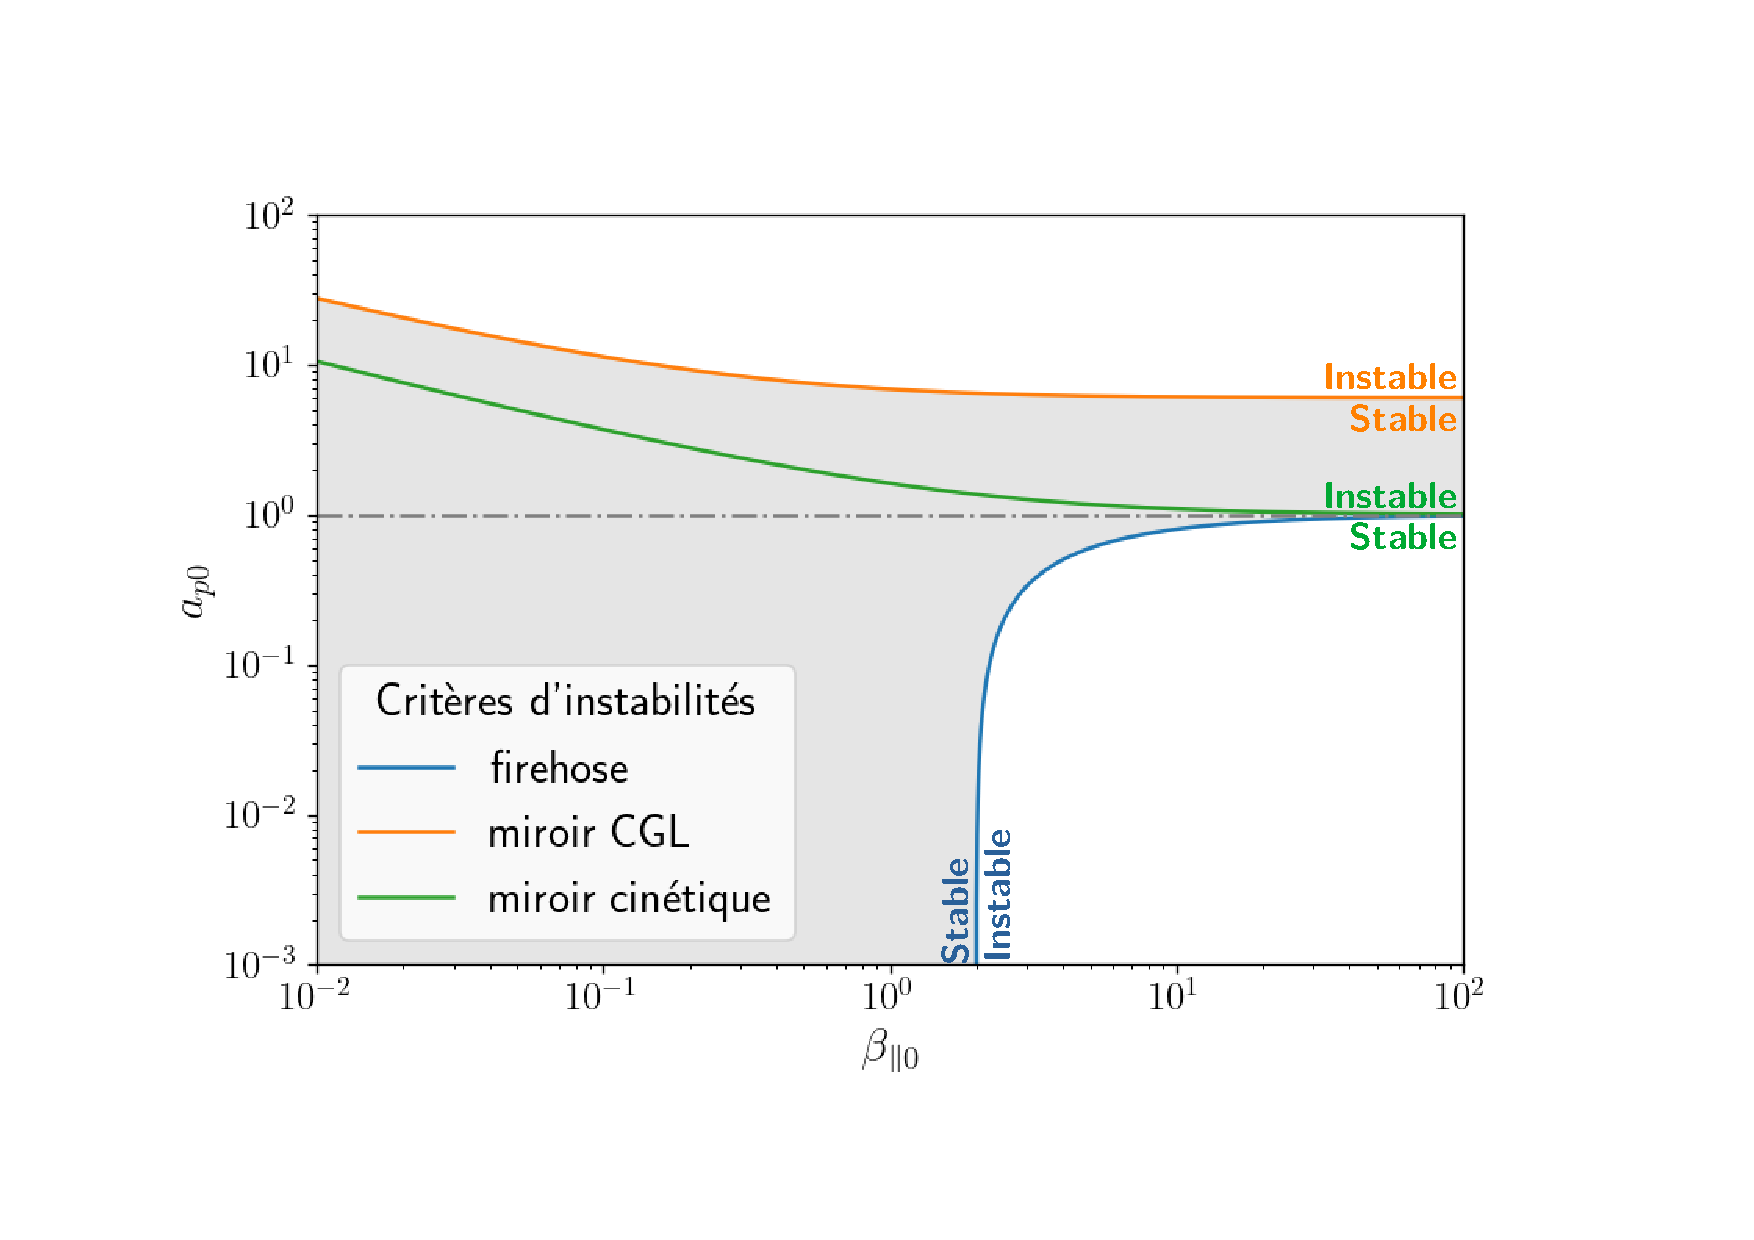
\includegraphics[width=0.9\linewidth,trim=3cm 2cm 4cm 3cm, clip=true]{./Mainmatter/Part_2/images/crit_diag_CGL}
\cprotect\caption{Zones de stabilité du modèle \cacro{CGL} (zone grisée). Critères d'instabilité firehose (bleu), miroir (orange) et miroir cinétique (vert). Horizontale \ensuremath{a_p=1} en gris.}
\label{fig:diag_cgl}
 \end{figure}
L'expression du critère d'instabilité miroir est légèrement différente de celle provenant de la théorie linéaire cinétique à cause du facteur $1/6$ [\cite{galeev_mhd_1983}, \cite{ferriere_mixed_2002}]. Ce facteur d'erreur translate la condition nécessaire pour qu'il y ait des instabilités miroir à $a_{p0}>6$ au lieu de $a_{p0}>1$, comme on peut le voir sur la \figref{fig:diag_cgl}. La condition nécessaire pour qu'il y ait apparition d'instabilité firehose est, quant à elle, $a_{p0}<1$ ce qui est en accord avec la théorie cinétique. Dans le vent solaire, ces critères d'instabilité semblent avoir un impact majeur puisque l'état du plasma semble maintenu, sur les diagrammes $a_p-\beta_{\parallel}$, dans une zone qu'ils semblent délimiter, comme l'a observé \cite{hellinger_solar_2006} dans les données relevées par la sonde \cacro{WIND}. 

Dans le Chapitre \ref{ch-11}, nous avons rappelé l'importance des ondes d'Alfvén dans les théories de turbulence et, dans le Chapitre \ref{ch-12}, que le sujet de l'impact des ondes compressibles \cacro{MHD} sur la cascade turbulente est toujours ouvert [\cite{brodiano_spatiotemporal_2021}]. Similairement, on peut se demander quel est l'impact des instabilités sur la turbulence ? Et en particulier, quelle est l'influence des instabilités des ondes d'Alfvén (firehose) sur la turbulence Alfvénique ? 

 Si l'on regarde les résultats des études de la température isotrope [\cite{liu_thermodynamic_2006}], des fluctuations magnétiques [\cite{bale_magnetic_2009}] et du taux de cascade incompressible [\cite{osman_proton_2013}] (voir \figref{fig:diag_osman}) dans les données relevées par \cacro{WIND} et ceux du taux compressible isotherme observés par \cite{hadid_compressible_2018} dans les données des missions \cacro{THEMIS} et \cacro{CLUSTER}, on remarque que sur les diagrammes $a_p-\beta_{\parallel}$, près des frontières des zones instables, la température des protons semble plus élevée, et les fluctuations du champ magnétique ainsi que les taux de cascade plus importants. Mais la relation entre instabilités et turbulence reste à clarifier : le plasma est-il plus chaud et turbulent parce que les instabilités jouent un rôle dans son chauffage ? Ce chauffage s'effectue-t-il via la cascade turbulente ? Ou est-ce lié à l'âge collisionnel du plasma comme le propose \cite{bale_magnetic_2009} ?
\begin{figure}[!ht]
 \centering
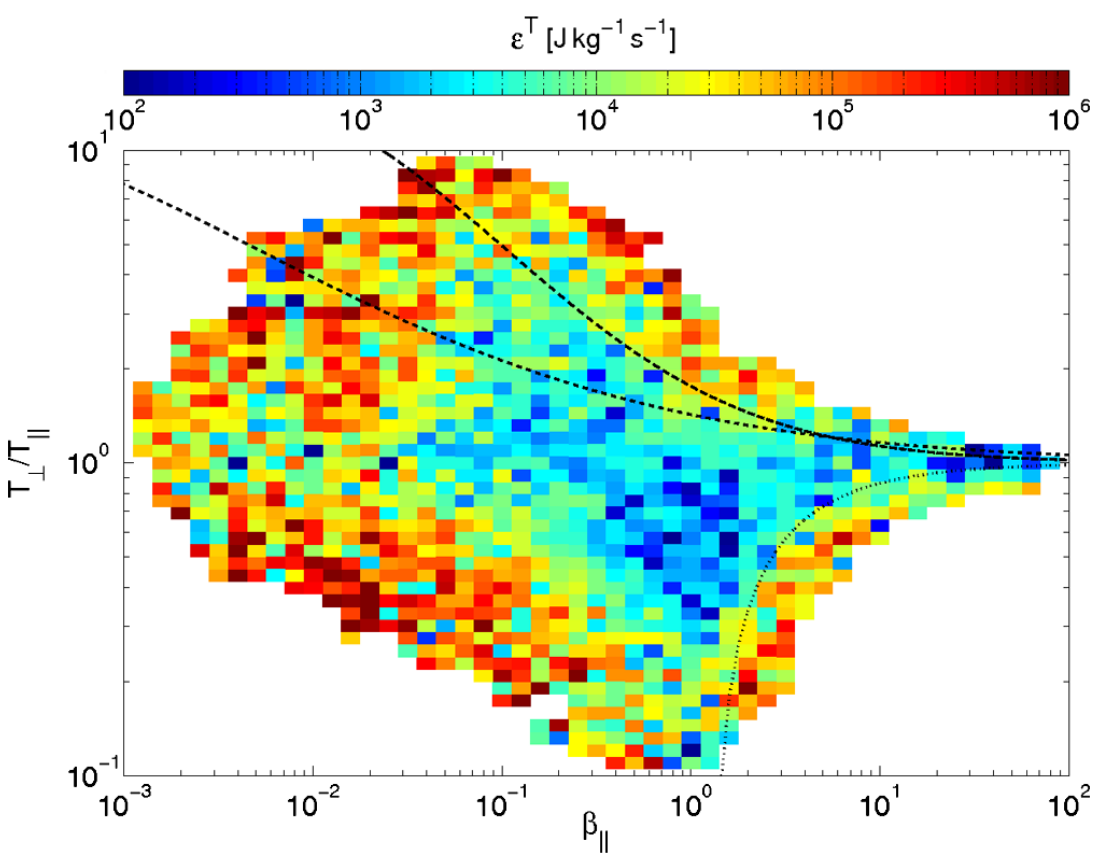
\includegraphics[width=0.8\linewidth,trim=0cm 0cm 0cm 0cm, clip=true]{./Mainmatter/Part_2/images/osman_2013}
\cprotect\caption{Distribution statistique en fonction de \ensuremath{a_p = \frac{p_{\perp}}{p_{\parallel}} =  \frac{T_{\perp}}{T_{\parallel}}} et \ensuremath{\beta_{\parallel}} d'échantillons relevés entre 1995 et 2011 dans le vent solaire par la sonde \cacro{WIND} en orbite autour de la Terre. Pour chacun d'eux, le taux de cascade est calculé avec la loi exacte \cacro{PP98} et indiqué par l'échelle chromatique. Les courbes pointillées indiquent les frontières associées aux instabilités cinétiques miroir (décroissante supérieure), cyclotron (décroissante inférieure) et firehose (croissante). [Crédits : \cite{osman_proton_2013}.]}
\label{fig:diag_osman}
\end{figure}

De multiples études se sont attaquées à ces questions à travers des comparaisons de spectres, du taux d'anisotropie de pression et des taux de croissance des instabilités cinétiques linéaires et quasi-linéaires. Parmi les plus récentes, on notera \cite{qudsi_intermittency_2020}, \cite{markovskii_effect_2022}, \cite{opie_conditions_2022}, \cite{bandyopadhyay_interplay_2022}, \cite{navarro_effects_2023}. 
De notre côté, nous l'attaquons analytiquement à partir des échelles fluides et de la théorie des lois exactes, dans le but d'offrir un cadre fluide permettant d'étudier plus rigoureusement l'impact des anisotropies et instabilités de pression sur la cascade turbulente.

\section{Loi exacte générale dépendant d'une pression tensorielle et loi CGL}
\label{sec-213}

Pour obtenir une loi exacte pour le modèle \ac{CGL}, nous avons utilisé la méthode mise en place dans le Chapitre \ref{ch-13}, c'est-à-dire prendre en compte l'équation d'énergie interne \eqref{eq:model_cpg_u} et non la forme explicite des pressions parallèle et perpendiculaire \eqref{eq:model_cpg_biadiab}. Le modèle utilisé est donc :
\begin{eqnarray}
\label{eq:turb_cpg_r} \partial_t \rho &=& - \nabla \cdot \left(\rho \boldsymbol{v}\right) , \\
\label{eq:turb_cpg_v}\partial_t  \boldsymbol{v} &=&- \nabla \cdot \left(\boldsymbol{v}\boldsymbol{v}\right) + \boldsymbol{v} \nabla \cdot \boldsymbol{v}  + \frac{1}{\rho} \nabla \cdot \left(\rho \boldsymbol{v_A}\boldsymbol{v_A}\right) - \frac{1}{\rho}  \nabla \cdot \overline{\boldsymbol{P_*}}  + \boldsymbol{f_c} + \boldsymbol{d_c} ,\\
\label{eq:turb_cpg_b}\partial_t \boldsymbol{v_A} &=&   \nabla \cdot \left(\boldsymbol{v_A}\boldsymbol{v} - \boldsymbol{v}\boldsymbol{v_A}\right) -  \boldsymbol{v}  \nabla \cdot \boldsymbol{v_A} +  \frac{\boldsymbol{v_A}}{2}  \nabla \cdot \boldsymbol{v} + \boldsymbol{f_m} + \boldsymbol{d_m} ,\\
\label{eq:turb_cpg_u}    \partial_t u  &=& - \nabla \cdot \left(u \boldsymbol{v} \right) + u  \nabla \cdot \boldsymbol{v}  -  \frac{\overline{\boldsymbol{P}}}{\rho} : \nabla \boldsymbol{v} . 
\end{eqnarray}

De manière cohérente avec les choix effectués dans le Chapitre \ref{ch-13}, la fonction de corrélation d'énergie totale choisie est $\mathcal{R} = \mathcal{R}_{c} + \mathcal{R}_{m} + \mathcal{R}_{u}$ avec $\mathcal{R}_{c} = \left<\frac{1}{4} \left(\rho'+\rho\right) \boldsymbol{v'} \cdot  \boldsymbol{v} \right>$, $\mathcal{R}_{m} = \left<\frac{1}{4} \left(\rho'+\rho\right) \boldsymbol{v'_A} \cdot  \boldsymbol{v_A} \right>$ et $\mathcal{R}_{u} = \frac{1}{2}\left< \rho' u + \rho u'\right> $. 

En appliquant la  même méthode que celle utilisée pour obtenir \eqref{eq:turb_cpi_Rc}, \eqref{eq:turb_cpi_Rm} et \eqref{eq:turb_cpi_Ru}, on obtient l'évolution temporelle des fonctions de corrélation associées à chaque énergie : 
\begin{itemize}
    \item Énergie cinétique : $\mathcal{R}_{c} = \left<\left(\rho'+\rho\right)\boldsymbol{v'} \cdot \boldsymbol{v}\right>/4 $
\begin{eqnarray}
\label{eq:turb_cpg_Rc} 4\partial_t \mathcal{R}_{c} &=& \nabla_{\boldsymbol{\ell}} \cdot \left<\delta \left(\rho\boldsymbol{v}\right) \cdot \delta \boldsymbol{v} \delta \boldsymbol{v} -\left(\delta \left(\rho\boldsymbol{v_A}\right) \cdot \delta \boldsymbol{v} \delta \boldsymbol{v_A} + \delta \left(\rho\boldsymbol{v}\right) \cdot \delta \boldsymbol{v_A} \delta \boldsymbol{v_A} \right)\right>\nonumber \\
&&+ \nabla_{\boldsymbol{\ell}} \cdot \left<\rho' \boldsymbol{v'_A}\cdot  \boldsymbol{v} \boldsymbol{v_A} -\rho \boldsymbol{v_A}\cdot  \boldsymbol{v'} \boldsymbol{v'_A}-\rho' \boldsymbol{v'} \cdot\boldsymbol{v_A}\boldsymbol{v'_A} +  \rho  \boldsymbol{v} \cdot\boldsymbol{v'_A}\boldsymbol{v_A}\right> \nonumber\\
& &+\left<\delta \boldsymbol{v}\cdot \left( \rho \boldsymbol{v}  \nabla' \cdot \boldsymbol{v'} -\rho' \boldsymbol{v'} \nabla \cdot \boldsymbol{v} \right)+2 \delta \boldsymbol{v_A}\cdot \left( \rho' \boldsymbol{v'} \nabla \cdot \boldsymbol{v_A} - \rho \boldsymbol{v} \right) \nabla' \cdot \boldsymbol{v'_A}\right> \nonumber\\
&&+  \nabla_{\boldsymbol{\ell}} \cdot \left< \rho' \frac{ \overline{\boldsymbol{P_*}}}{\rho} \cdot \boldsymbol{v'} -  \rho \frac{\overline{\boldsymbol{P'_*}}}{\rho'} \cdot \boldsymbol{v} + \overline{\boldsymbol{P_*}} \cdot \boldsymbol{v'} -  \overline{\boldsymbol{P'_*}} \cdot \boldsymbol{v} \right>\nonumber \\
&&- \left<\frac{\rho'}{\rho} \boldsymbol{v'} \cdot \overline{\boldsymbol{P_*}}  \cdot \frac{\nabla \rho}{\rho} + \frac{\rho}{\rho'} \boldsymbol{v} \cdot \overline{\boldsymbol{P'_*}}   \cdot \frac{\nabla' \rho'}{\rho'} \right>\nonumber\\
&&+  \left<\left(\rho' + \rho\right)\left(\boldsymbol{v} \cdot \boldsymbol{f'_c} + \boldsymbol{v'} \cdot \boldsymbol{f_c}\right) \right>+ \left<\left(\rho' + \rho\right)\left(\boldsymbol{v} \cdot \boldsymbol{d'_c} + \boldsymbol{v'} \cdot \boldsymbol{d_c}\right)\right> .
\end{eqnarray}
    \item Énergie magnétique : $\mathcal{R}_{m} = \left<\left(\rho'+\rho\right)\boldsymbol{v'_A} \cdot \boldsymbol{v_A}\right>/4 $
\begin{eqnarray}
\label{eq:turb_cpg_Rm} 4\partial_t \mathcal{R}_{m} &=& \nabla_{\boldsymbol{\ell}} \cdot \left<\delta \left(\rho\boldsymbol{v_A}\right) \cdot \delta \boldsymbol{v_A} \delta \boldsymbol{v} \right> \nonumber\\
&&-\nabla_{\boldsymbol{\ell}} \cdot \left< \rho' \boldsymbol{v'_A}\cdot  \boldsymbol{v} \boldsymbol{v_A} - \rho \boldsymbol{v_A}\cdot  \boldsymbol{v'} \boldsymbol{v'_A}-\rho' \boldsymbol{v'} \cdot\boldsymbol{v_A}\boldsymbol{v'_A} +  \rho  \boldsymbol{v} \cdot\boldsymbol{v'_A}\boldsymbol{v_A}\right> \nonumber\\
&&+ \left<\left(\rho \boldsymbol{v_A} \cdot \delta \boldsymbol{v_A} -\frac{1}{2} \left(\rho'+\rho\right) \boldsymbol{v'_A} \cdot \boldsymbol{v_A}\right)\nabla' \cdot \boldsymbol{v'}\right> \nonumber\\
&&-  \left<\left(\rho' \boldsymbol{v'_A} \cdot \delta \boldsymbol{v_A} + \frac{1}{2} \left(\rho'+\rho\right) \boldsymbol{v'_A} \cdot \boldsymbol{v_A}\right)\nabla \cdot \boldsymbol{v}\right>\nonumber\\
&& + \left<\left( \rho' \boldsymbol{v'_A} \cdot \boldsymbol{v} - \rho \boldsymbol{v} \cdot \boldsymbol{v'_A}  \right)\nabla \cdot \boldsymbol{v_A} \right> + \left<\left(\rho' \boldsymbol{v'} \cdot \boldsymbol{v_A} -  \rho \boldsymbol{v_A} \cdot \boldsymbol{v'} \right)\nabla' \cdot \boldsymbol{v'_A} \right>\nonumber\\
&&+  \left<\left(\rho' + \rho\right)\left(\boldsymbol{v_A} \cdot \boldsymbol{f'_m} + \boldsymbol{v'_A} \cdot \boldsymbol{f_m}\right) \right>+ \left<\left(\rho' + \rho\right)\left(\boldsymbol{v_A} \cdot \boldsymbol{d'_m} + \boldsymbol{v'_A} \cdot \boldsymbol{d_m}\right)\right> .\nonumber\\
\end{eqnarray}
    \item Énergie interne :  $\mathcal{R}_{u} = \left<\rho' u+\rho u'\right>/2 $
\begin{eqnarray}
\label{eq:turb_cpg_Ru} 2\partial_t \mathcal{R}_{u} &=&\nabla_{\boldsymbol{\ell}} \cdot \left<\delta \rho  \delta u \delta \boldsymbol{v} \right> + \left<  \rho \delta u \nabla' \cdot \boldsymbol{v'}- \rho' \delta u \nabla \cdot \boldsymbol{v}\right> \nonumber\\
&&-\left< \rho' \frac{\overline{\boldsymbol{P}}}{\rho} :  \nabla  \boldsymbol{v}  + \rho \frac{\overline{\boldsymbol{P'}}}{\rho'} : \nabla'  \boldsymbol{v'} \right> .
\end{eqnarray}
\end{itemize}
Le résultat pour l'énergie magnétique n'est pas influencé par le type de pression (tensoriel ou isotrope) contrairement à ceux des énergies cinétique et interne. La question qui s'est posée alors était : est-il possible d'améliorer la formulation des termes dépendant de la pression ? Autrement dit, est-il possible de faire apparaître l'influence de la pression dans les termes de type flux sous la forme d'une fonction de structure ?
 En remarquant que $\overline{\boldsymbol{P}}$ ou $\overline{\boldsymbol{P_*}}$ est, dans tous les termes, accompagné de $\frac{1}{\rho}$ pris au même point, l'idée de travailler sur la fonction de structure $\left<\delta \rho \delta \frac{ \overline{\boldsymbol{P}}}{\rho} \cdot \delta \boldsymbol{v} \right>$ puis sur la fonction $\left<\delta \rho \delta \frac{ \overline{\boldsymbol{P_*}} }{\rho} \cdot\delta \boldsymbol{v} \right>$ a émergé. Développer cette dernière sous la divergence locale en utilisant l'hypothèse d'homogénéité statistique et l'indépendance des positions $\boldsymbol{x}$ et  $\boldsymbol{x'}$ donne alors : 
\begin{eqnarray*}
    \nabla_{\boldsymbol{\ell}} \cdot \left<\delta \rho \delta \frac{ \overline{\boldsymbol{P_*}} }{\rho}  \cdot\delta \boldsymbol{v} \right> &=& \nabla_{\boldsymbol{\ell}} \cdot \left< \left[\rho  \frac{ \overline{\boldsymbol{P'_*}} }{\rho'}   \cdot\boldsymbol{v}  -\rho'  \frac{ \overline{\boldsymbol{P_*}} }{\rho} \cdot \boldsymbol{v'}\right] +  \left[\overline{\boldsymbol{P_*}} \cdot \boldsymbol{v'} - \overline{\boldsymbol{P'_*}}    \cdot\boldsymbol{v} \right] \right> \\
    &&+\nabla_{\boldsymbol{\ell}} \cdot \left<\rho'  \frac{ \overline{\boldsymbol{P_*}} }{\rho} \cdot \boldsymbol{v} - \rho  \frac{ \overline{\boldsymbol{P'_*}} }{\rho'}  \cdot \boldsymbol{v'}  \right> .
\end{eqnarray*}
 On peut donc exprimer $ \nabla_{\boldsymbol{\ell}} \cdot \left< \rho' \frac{ \overline{\boldsymbol{P_*}}}{\rho} \cdot \boldsymbol{v'} -  \rho \frac{\overline{\boldsymbol{P'_*}}}{\rho'} \cdot \boldsymbol{v} \right>$ ou $ \nabla_{\boldsymbol{\ell}} \cdot \left<  \overline{\boldsymbol{P_*}} \cdot \boldsymbol{v'} -  \overline{\boldsymbol{P'_*}} \cdot \boldsymbol{v} \right>$ en fonction de $\left<\delta \rho \delta \frac{ \overline{\boldsymbol{P_*}} }{\rho} \cdot\delta \boldsymbol{v} \right>$ dans \eqref{eq:turb_cpg_Rc}. Sachant que 
 \begin{equation*}
  \nabla_{\boldsymbol{\ell}} \cdot \left<  \overline{\boldsymbol{P_*}} \cdot \boldsymbol{v'} -  \overline{\boldsymbol{P'_*}} \cdot \boldsymbol{v} \right> = \left<  \rho  \frac{ \overline{\boldsymbol{P_*}} }{\rho} : \nabla'\boldsymbol{v'} +   \rho'\frac{ \overline{\boldsymbol{P'_*}} }{\rho'} : \nabla \boldsymbol{v} \right>
 \end{equation*}
 rappellant les termes dépendant de la pression dans l'équation \eqref{eq:turb_cpg_Ru}, nous avons choisi la première possibilité. Ainsi : 
\begin{eqnarray*}
\nabla_{\boldsymbol{\ell}} &\cdot& \left< \rho' \frac{ \overline{\boldsymbol{P_*}}}{\rho} \cdot \boldsymbol{v'} -  \rho \frac{\overline{\boldsymbol{P'_*}}}{\rho'} \cdot \boldsymbol{v}  +  \overline{\boldsymbol{P_*}} \cdot \boldsymbol{v'} -  \overline{\boldsymbol{P'_*}} \cdot \boldsymbol{v} \right>\\
&=& -\nabla_{\boldsymbol{\ell}} \cdot \left<\delta \rho \delta \frac{ \overline{\boldsymbol{P_*}} }{\rho} \cdot \delta \boldsymbol{v} \right> +  \left<   \boldsymbol{v}\cdot\frac{ \overline{\boldsymbol{P_*}} }{\rho} \cdot  \nabla'\rho' + \boldsymbol{v'} \cdot \frac{ \overline{\boldsymbol{P'_*}} }{\rho'} \cdot \nabla \rho  \right> \\
&&+ \left< 2 \rho  \frac{ \overline{\boldsymbol{P}} }{\rho} : \nabla'\boldsymbol{v'} + 2  \rho'\frac{ \overline{\boldsymbol{P'}} }{\rho'} : \nabla \boldsymbol{v}  + \rho \boldsymbol{v_A}^2 \nabla' \cdot \boldsymbol{v'} +   \rho' \boldsymbol{v'_A}^2 \nabla \cdot \boldsymbol{v}\right> .
\end{eqnarray*}

La loi \cacro{KHM} générale pour l'énergie totale avec $\mathcal{R} = \mathcal{R}_{c} + \mathcal{R}_{m} + \mathcal{R}_{u}$ devient alors :
\begin{equation}
\label{eq:turb_cpg_khm} \boxed{
\begin{array}{lcl}
{}_{[1]} \quad 4\partial_t \mathcal{R} &=& \nabla_{\boldsymbol{\ell}} \cdot \left<\left(\delta \left(\rho\boldsymbol{v}\right) \cdot \delta \boldsymbol{v}+ \delta \left(\rho\boldsymbol{v_A}\right) \cdot \delta \boldsymbol{v_A} \right) \delta \boldsymbol{v}  -\left(\delta \left(\rho\boldsymbol{v_A}\right) \cdot \delta \boldsymbol{v}  + \delta \left(\rho\boldsymbol{v}\right) \cdot \delta \boldsymbol{v_A}  \right) \delta \boldsymbol{v_A} \right>\\
{}_{[2]} && +\left< \left(\rho \boldsymbol{v} \cdot \delta \boldsymbol{v} +\frac{1}{2} \rho \boldsymbol{v_A} \cdot  \delta \boldsymbol{v_A} -\frac{1}{2} \delta \left(\rho \boldsymbol{v_A}\right) \cdot \boldsymbol{v_A} \right) \nabla' \cdot \boldsymbol{v'} \right>\\
{}_{[3]} && -\left< \left(\rho' \boldsymbol{v'} \cdot \delta \boldsymbol{v}  + \frac{1}{2} \rho' \boldsymbol{v'_A} \cdot \delta \boldsymbol{v_A}  - \frac{1}{2} \delta \left(\rho \boldsymbol{v_A}\right) \cdot \boldsymbol{v'_A}  \right)\nabla \cdot \boldsymbol{v}\right>\\
{}_{[4]} &&+ \left<\left(2 \rho' \boldsymbol{v'} \cdot \delta \boldsymbol{v_A}- \delta \left(\rho \boldsymbol{v}\right) \cdot \boldsymbol{v'_A} + \rho' \boldsymbol{v'_A} \cdot \delta \boldsymbol{v}  \right)\nabla \cdot \boldsymbol{v_A}\right>\\
{}_{[5]} &&- \left<\left(2\rho \boldsymbol{v} \cdot \delta \boldsymbol{v_A} - \delta \left(\rho \boldsymbol{v}\right) \cdot \boldsymbol{v_A} +  \rho \boldsymbol{v_A} \cdot \delta \boldsymbol{v} \right)\nabla' \cdot \boldsymbol{v'_A}\right> \\
{}_{[6]} &&+ \nabla_{\boldsymbol{\ell}} \cdot \left< 2\delta \rho  \delta u \delta \boldsymbol{v}\right> + 2\left<\rho \delta u \nabla' \cdot \boldsymbol{v'}- \rho' \delta u \nabla \cdot \boldsymbol{v}\right>\\
{}_{[7]} &&- \nabla_{\boldsymbol{\ell}} \cdot \left<\delta \rho \delta \frac{ \overline{\boldsymbol{P_*}} }{\rho} \cdot \delta \boldsymbol{v} \right> - 2\left<\rho \delta \frac{ \overline{\boldsymbol{P}} }{\rho}:\nabla' \boldsymbol{v'} -  \rho' \delta \frac{ \overline{\boldsymbol{P}} }{\rho} :\nabla  \boldsymbol{v} \right>\\
{}_{[8]} && +  \left< \boldsymbol{v} \cdot \left(  \frac{ \overline{\boldsymbol{P_*}} }{\rho} \delta \rho - \rho \delta \frac{ \overline{\boldsymbol{P_*}} }{\rho}  \right)\cdot  \frac{\nabla' \rho'}{\rho'} - \boldsymbol{v'} \cdot \left(  \frac{ \overline{\boldsymbol{P'_*}} }{\rho'} \delta \rho - \rho' \delta \frac{ \overline{\boldsymbol{P_*}} }{\rho}  \right)\cdot  \frac{\nabla \rho}{\rho}  \right>\\
{}_{[9]}&&+  \left<\left(\rho' + \rho\right)\left(\boldsymbol{v} \cdot \boldsymbol{f'_c} + \boldsymbol{v'} \cdot \boldsymbol{f_c} + \boldsymbol{v_A} \cdot \boldsymbol{f'_m} + \boldsymbol{v'_A} \cdot \boldsymbol{f_m}\right) \right>\\
{}_{[10]}&&+ \left<\left(\rho' + \rho\right)\left(\boldsymbol{v} \cdot \boldsymbol{d'_c} + \boldsymbol{v'} \cdot \boldsymbol{d_c}+\boldsymbol{v_A} \cdot \boldsymbol{d'_m} + \boldsymbol{v'_A} \cdot \boldsymbol{d_m}\right)\right> .
\end{array}}
\end{equation} 
 Les lignes [7] et [8] contiennent les contributions des tenseurs de pression et de pression totale. 
 
La loi exacte générale de type \cacro{K41} est alors : 
\begin{equation}
\label{eq:turb_cpg_elk} \boxed{
\begin{array}{lcl}
- 4\varepsilon &=& \nabla_{\boldsymbol{\ell}} \cdot \left<\left(\delta \left(\rho\boldsymbol{v}\right) \cdot \delta \boldsymbol{v}+ \delta \left(\rho\boldsymbol{v_A}\right) \cdot \delta \boldsymbol{v_A} \right) \delta \boldsymbol{v}  -\left(\delta \left(\rho\boldsymbol{v_A}\right) \cdot \delta \boldsymbol{v}  + \delta \left(\rho\boldsymbol{v}\right) \cdot \delta \boldsymbol{v_A}  \right) \delta \boldsymbol{v_A} \right>\\
&&+ \nabla_{\boldsymbol{\ell}} \cdot \left< 2\delta \rho  \delta u \delta \boldsymbol{v}-\delta \rho \delta \frac{ \overline{\boldsymbol{P_*}} }{\rho} \cdot \delta \boldsymbol{v} \right> \\
&& +\left< \left(\rho \boldsymbol{v} \cdot \delta \boldsymbol{v} +\frac{1}{2} \rho \boldsymbol{v_A} \cdot  \delta \boldsymbol{v_A} -\frac{1}{2} \delta \left(\rho \boldsymbol{v_A}\right) \cdot \boldsymbol{v_A} +2\rho \delta u\right) \nabla' \cdot \boldsymbol{v'} -2\rho \delta \frac{ \overline{\boldsymbol{P}} }{\rho}:\nabla' \boldsymbol{v'}\right>\\
 && -\left< \left(\rho' \boldsymbol{v'} \cdot \delta \boldsymbol{v}  + \frac{1}{2} \rho' \boldsymbol{v'_A} \cdot \delta \boldsymbol{v_A}  - \frac{1}{2} \delta \left(\rho \boldsymbol{v_A}\right) \cdot \boldsymbol{v'_A}  +2\rho' \delta u\right)\nabla \cdot \boldsymbol{v} - 2\rho' \delta \frac{ \overline{\boldsymbol{P}} }{\rho} :\nabla  \boldsymbol{v}\right>\\
&&+ \left<\left(2 \rho' \boldsymbol{v'} \cdot \delta \boldsymbol{v_A}- \delta \left(\rho \boldsymbol{v}\right) \cdot \boldsymbol{v'_A} + \rho' \boldsymbol{v'_A} \cdot \delta \boldsymbol{v}  \right)\nabla \cdot \boldsymbol{v_A}\right>\\
 &&- \left<\left(2\rho \boldsymbol{v} \cdot \delta \boldsymbol{v_A} - \delta \left(\rho \boldsymbol{v}\right) \cdot \boldsymbol{v_A} +  \rho \boldsymbol{v_A} \cdot \delta \boldsymbol{v} \right)\nabla' \cdot \boldsymbol{v'_A}\right> \\
&& +  \left< \boldsymbol{v} \cdot \left(  \frac{ \overline{\boldsymbol{P_*}} }{\rho} \delta \rho - \rho \delta \frac{ \overline{\boldsymbol{P_*}} }{\rho}  \right)\cdot  \frac{\nabla' \rho'}{\rho'} - \boldsymbol{v'} \cdot \left(  \frac{ \overline{\boldsymbol{P'_*}} }{\rho'} \delta \rho - \rho' \delta \frac{ \overline{\boldsymbol{P_*}} }{\rho}  \right)\cdot  \frac{\nabla \rho}{\rho}  \right>.
\end{array}}
\end{equation}
Cette loi est valable quelle que soit la forme du tenseur de pression ou de l'énergie interne tant que la zone inertielle est supposée isentrope. Si l'on considère la pression sous forme isotrope $\overline{\boldsymbol{P}} = p \overline{\boldsymbol{I}}$, on trouve la loi \eqref{eq:turb_elg_f2} analysée dans la section \ref{sec-132}. On notera ce résultat $\varepsilon_{iso}$. On peut alors isoler dans le taux de cascade la contribution de la composante anisotrope du tenseur de pression $\overline{\boldsymbol{\Pi}}$ : 
\begin{equation}
\label{eq:turb_cpgyr_an} \boxed{
\begin{array}{lcl}
- 4\left(\varepsilon - \varepsilon_{iso}\right) &=& - \nabla_{\boldsymbol{\ell}} \cdot \left< \delta \rho \delta \left(\frac{\overline{\boldsymbol{\Pi}}}{\rho}\right) \cdot \delta \boldsymbol{v} \right>  -\left< 2\rho \delta \left(\frac{\overline{\boldsymbol{\Pi}}}{\rho}\right):\nabla' \boldsymbol{v'} -  2\rho' \delta \left(\frac{\overline{\boldsymbol{\Pi}}}{\rho}\right) :\nabla  \boldsymbol{v}\right>\\
&& +  \left< \boldsymbol{v} \cdot \left(  \left(\frac{\overline{\boldsymbol{\Pi}}}{\rho}\right) \delta \rho - \rho \delta \left(\frac{\overline{\boldsymbol{\Pi}}}{\rho}\right)  \right)\cdot  \frac{\nabla' \rho'}{\rho'}-\boldsymbol{v'} \cdot \left(  \left(\frac{\overline{\boldsymbol{\Pi'}}}{\rho'}\right) \delta \rho - \rho' \delta \left(\frac{\overline{\boldsymbol{\Pi}}}{\rho}\right)  \right)\cdot  \frac{\nabla \rho}{\rho}  \right>.
\end{array}}
\end{equation}
Nous quantifierons et analyserons cette contribution grâce à des simulations dans la Partie \ref{part_3}. 

Dans le cas d'un tenseur de pression gyrotrope, on peut faire apparaître $p_{\parallel}$ et $p_{\perp}$ : 
\begin{equation}
\label{eq:turb_cpgyr_elk}% \boxed{
\begin{array}{lcl}
%\begin{eqnarray}
%\label{eq:turb_cpgyr_elk} 
- 4\varepsilon &=& \nabla_{\boldsymbol{\ell}} \cdot \left<\left(\delta \left(\rho\boldsymbol{v}\right) \cdot \delta \boldsymbol{v}+ \delta \left(\rho\boldsymbol{v_A}\right) \cdot \delta \boldsymbol{v_A} \right)\delta \boldsymbol{v}  -\left(\delta \left(\rho\boldsymbol{v_A}\right) \cdot \delta \boldsymbol{v}  + \delta \left(\rho\boldsymbol{v}\right) \cdot \delta \boldsymbol{v_A}  \right) \delta \boldsymbol{v_A} \right>\\
&+& \nabla_{\boldsymbol{\ell}} \cdot \left< \delta \rho  \delta \left(\frac{p_{\perp} + p_{\parallel}+p_m}{\rho}\right) \delta \boldsymbol{v}+\delta \rho \delta \left(\frac{p_{\perp} - p_{\parallel}}{\rho}\boldsymbol{b}\boldsymbol{b}\right) \cdot \delta \boldsymbol{v} \right> \\
& +&\left< \left(\rho \boldsymbol{v} \cdot \delta \boldsymbol{v} +\frac{1}{2} \rho \boldsymbol{v_A} \cdot  \delta \boldsymbol{v_A} -\frac{1}{2} \delta \left(\rho \boldsymbol{v_A}\right) \cdot \boldsymbol{v_A} +\rho \delta \left(\frac{p_{\parallel}}{\rho}\right)\right) \nabla' \cdot \boldsymbol{v'} \right>\\
 & -&\left< \left(\rho' \boldsymbol{v'} \cdot \delta \boldsymbol{v}  + \frac{1}{2} \rho' \boldsymbol{v'_A} \cdot \delta \boldsymbol{v_A}  - \frac{1}{2} \delta \left(\rho \boldsymbol{v_A}\right) \cdot \boldsymbol{v'_A}  +\rho' \delta \left(\frac{p_{\parallel}}{\rho}\right)\right)\nabla \cdot \boldsymbol{v} \right>\\
 &+&2\left<\rho \delta \left(\frac{p_{\perp} - p_{\parallel}}{\rho}\boldsymbol{b}\boldsymbol{b}\right):\nabla' \boldsymbol{v'} - \rho' \delta \left(\frac{p_{\perp} - p_{\parallel}}{\rho}\boldsymbol{b}\boldsymbol{b}\right) :\nabla  \boldsymbol{v}\right>\\
&+& \left<\left(2 \rho' \boldsymbol{v'} \cdot \delta \boldsymbol{v_A}- \delta \left(\rho \boldsymbol{v}\right) \cdot \boldsymbol{v'_A} + \rho' \boldsymbol{v'_A} \cdot \delta \boldsymbol{v}  \right)\nabla \cdot \boldsymbol{v_A}\right>\\
 &-& \left<\left(2\rho \boldsymbol{v} \cdot \delta \boldsymbol{v_A} - \delta \left(\rho \boldsymbol{v}\right) \cdot \boldsymbol{v_A} +  \rho \boldsymbol{v_A} \cdot \delta \boldsymbol{v} \right)\nabla' \cdot \boldsymbol{v'_A}\right>\\
   %& +&  \left< \delta \rho  \left( \left( \frac{p_{\perp}+p_m }{\rho} \boldsymbol{v} +  \frac{ p_{\parallel}-p_{\perp}}{\rho} \boldsymbol{v} \cdot\boldsymbol{b}\boldsymbol{b}   \right)\cdot  \frac{\nabla' \rho'}{\rho'} - \left(\frac{ p'_{\perp}+p'_m }{\rho'} \boldsymbol{v'}+ \frac{ p'_{\parallel}-p'_{\perp}}{\rho'}\boldsymbol{v'} \cdot\boldsymbol{b'}\boldsymbol{b'}\right)\cdot  \frac{\nabla \rho}{\rho}\right)   \right>\nonumber \\
   %- \delta \left(\frac{ p_{\perp}+p_m }{\rho}\right) \left(\rho \boldsymbol{v} \cdot  \frac{\nabla' \rho'}{\rho'} -  \rho' \boldsymbol{v'}\cdot  \frac{\nabla \rho}{\rho}\right)  \right>\nonumber \\
  % &+& \left<  \delta \rho\left( \frac{ p_{\parallel}-p_{\perp}}{\rho} \boldsymbol{v} \cdot\boldsymbol{b}\boldsymbol{b}   \cdot  \frac{\nabla' \rho'}{\rho'} - \frac{ p'_{\parallel}-p'_{\perp}}{\rho'}\boldsymbol{v'} \cdot\boldsymbol{b'}\boldsymbol{b'}  \cdot  \frac{\nabla \rho}{\rho}\right)
  % -  \delta \left(\frac{ p_{\parallel}-p_{\perp}}{\rho}\boldsymbol{b}\boldsymbol{b} \right) : \left( \rho  \boldsymbol{v}  \frac{\nabla' \rho'}{\rho'} - \rho' \boldsymbol{v'}   \frac{\nabla \rho}{\rho} \right)\right>\nonumber \\
  & +&  \left<  \left(  \frac{p_{\perp}+p_m }{\rho} \boldsymbol{v}\delta \rho - \rho \boldsymbol{v}\delta \left(\frac{ p_{\perp}+p_m }{\rho}\right) \right)\cdot  \frac{\nabla' \rho'}{\rho'} \right>\\
  &+&  \left<  \left(    \frac{ p_{\parallel}-p_{\perp}}{\rho} \boldsymbol{v} \cdot\boldsymbol{b}\boldsymbol{b} \delta \rho -\rho  \boldsymbol{v} \cdot \delta \left(\frac{ p_{\parallel}-p_{\perp}}{\rho}\boldsymbol{b}\boldsymbol{b} \right)  \right)\cdot  \frac{\nabla' \rho'}{\rho'} \right>\\
 &-& \left< \left(  \frac{ p'_{\perp}+p'_m }{\rho'} \boldsymbol{v'}\delta \rho - \rho' \boldsymbol{v'}\delta \left(\frac{ p_{\perp}+p_m }{\rho}\right) \right) \cdot  \frac{\nabla \rho}{\rho} \right>\\
 &-&   \left< \left(  \frac{ p'_{\parallel}-p'_{\perp}}{\rho'}\boldsymbol{v'} \cdot\boldsymbol{b'}\boldsymbol{b'}  \delta \rho - \rho' \boldsymbol{v'} \cdot\delta \left(\frac{ p_{\parallel}-p_{\perp}}{\rho}\boldsymbol{b}\boldsymbol{b} \right)\right) \cdot  \frac{\nabla \rho}{\rho} \right> .
%\end{eqnarray}
\end{array}%}
\end{equation}
Cette loi est valable pour le modèle \cacro{CGL}. Si besoin est, on peut y expliciter $p_{\parallel}$ et $p_{\perp}$ en fonction de $\rho$, $\boldsymbol{v_A}$ grâce à \eqref{eq:model_cpg_biadiab}. 

On peut aussi faire apparaître $a_p$ et $\beta_{\parallel}$ dans \eqref{eq:turb_cpgyr_elk} pour identifier les termes potentiellement impactés par les instabilités. Ainsi, on obtient :  
\begin{equation}
\label{eq:turb_cpinst_elk} \boxed{
\begin{array}{lcl}
- 4\varepsilon &=& \nabla_{\boldsymbol{\ell}} \cdot \left<\left(\delta \left(\rho\boldsymbol{v}\right) \cdot \delta \boldsymbol{v}+ \delta \left(\rho\boldsymbol{v_A}\right) \cdot \delta \boldsymbol{v_A} \right) \delta \boldsymbol{v}  -\left(\delta \left(\rho\boldsymbol{v_A}\right) \cdot \delta \boldsymbol{v}  + \delta \left(\rho\boldsymbol{v}\right) \cdot \delta \boldsymbol{v_A}  \right) \delta \boldsymbol{v_A} \right>\\
&&+ \frac{1}{2}\nabla_{\boldsymbol{\ell}} \cdot \left< \delta \rho  \delta \left(\boldsymbol{v_A}^2 \left(\beta_{\parallel}\left(a_p+1\right)+1\right)\right) \delta \boldsymbol{v}+\delta \rho \delta \left(\beta_{\parallel}\left(a_p-1\right) \boldsymbol{v_A} \boldsymbol{v_A}\right) \cdot \delta \boldsymbol{v} \right> \\
&& +\left< \left(\rho \boldsymbol{v} \cdot \delta \boldsymbol{v} +\frac{1}{2} \rho \boldsymbol{v_A} \cdot  \delta \boldsymbol{v_A} -\frac{1}{2} \delta \left(\rho \boldsymbol{v_A}\right) \cdot \boldsymbol{v_A} + \frac{1}{2}\rho \delta \left(\boldsymbol{v_A}^2 \beta_{\parallel}\right)\right) \nabla' \cdot \boldsymbol{v'} \right>\\
 && -\left< \left(\rho' \boldsymbol{v'} \cdot \delta \boldsymbol{v}  + \frac{1}{2} \rho' \boldsymbol{v'_A} \cdot \delta \boldsymbol{v_A}  - \frac{1}{2} \delta \left(\rho \boldsymbol{v_A}\right) \cdot \boldsymbol{v'_A}  + \frac{1}{2} \rho' \delta \left(\boldsymbol{v_A}^2 \beta_{\parallel}\right)\right)\nabla \cdot \boldsymbol{v} \right>\\
 &&+\left<\rho \delta \left(\beta_{\parallel}\left(a_p-1\right) \boldsymbol{v_A} \boldsymbol{v_A}\right):\nabla' \boldsymbol{v'} - \rho' \delta \left(\beta_{\parallel}\left(a_p-1\right) \boldsymbol{v_A} \boldsymbol{v_A}\right) :\nabla  \boldsymbol{v}\right>\\
&&+ \left<\left(2 \rho' \boldsymbol{v'} \cdot \delta \boldsymbol{v_A}- \delta \left(\rho \boldsymbol{v}\right) \cdot \boldsymbol{v'_A} + \rho' \boldsymbol{v'_A} \cdot \delta \boldsymbol{v}  \right)\nabla \cdot \boldsymbol{v_A}\right>\\
 &&- \left<\left(2\rho \boldsymbol{v} \cdot \delta \boldsymbol{v_A} - \delta \left(\rho \boldsymbol{v}\right) \cdot \boldsymbol{v_A} +  \rho \boldsymbol{v_A} \cdot \delta \boldsymbol{v} \right)\nabla' \cdot \boldsymbol{v'_A}\right> \\
&& + \frac{1}{2} \left<  \left(  \boldsymbol{v_A}^2 \left(\beta_{\parallel}a_p+1\right) \delta \rho - \rho \delta \left(\boldsymbol{v_A}^2 \left(\beta_{\parallel}a_p+1\right)\right)  \right)\boldsymbol{v}\cdot  \frac{\nabla' \rho'}{\rho'} \right>\\
&&- \frac{1}{2} \left<\left(  \boldsymbol{v'_A}^2 \left(\beta'_{\parallel}a'_p+1\right) \delta \rho - \rho' \delta \left(\boldsymbol{v_A}^2 \left(\beta_{\parallel}a_p+1\right)\right)  \right) \boldsymbol{v'}\cdot  \frac{\nabla \rho}{\rho}  \right> \\
&& + \frac{1}{2} \left< \boldsymbol{v} \cdot \left(  \beta_{\parallel}\left(a_p-1\right) \boldsymbol{v_A} \boldsymbol{v_A} \delta \rho - \rho \delta \left(\beta_{\parallel}\left(a_p-1\right) \boldsymbol{v_A} \boldsymbol{v_A}\right)  \right)\cdot  \frac{\nabla' \rho'}{\rho'} \right>\\
&&-\frac{1}{2}\left< \boldsymbol{v'} \cdot \left( \beta'_{\parallel}\left(a'_p-1\right) \boldsymbol{v'_A} \boldsymbol{v'_A}  \delta \rho - \rho' \delta \left(\beta_{\parallel}\left(a_p-1\right) \boldsymbol{v_A} \boldsymbol{v_A} \right)\right) \cdot  \frac{\nabla \rho}{\rho} \right>.
\end{array}}
\end{equation}
Les critères d'instabilité linéaires n'y sont pas explicites, mais on observe que certains termes, présents dans la contribution anisotrope \eqref{eq:turb_cpgyr_an}, dépendent de $a_p-1$, en particulier le terme de type flux. Par conséquent, le signe de ces termes va dépendre du régime de pression dans le système, c'est-à-dire si $p_{\parallel}$ ou $p_{\perp}$ domine, et est ainsi lié au type d'instabilité pouvant s'y développer. Comme ces termes dépendent de quantités incrémentales, il est néanmoins difficile de conclure sur leur apport au taux de cascade total sans regarder dans des simulations. Ce sera l'un des objectifs de la Partie \ref{part_3}.

\newpage
\section{Synthèse de l'étude analytique de turbulence compressible avec pression tensorielle et modèle CGL}
\label{synt-21}

 \fcolorbox{blue}{white}{\begin{minipage}[c]{\linewidth}
 \paragraph{Fermeture CGL : } $\nabla \cdot \overline{\overline{\boldsymbol{q}}}=0$ et $\overline{\boldsymbol{P}}  = p \overline{\boldsymbol{I}} + \overline{\boldsymbol{\Pi}}=  \frac{2 p_{\perp} + p_{\parallel}}{3}  \overline{\boldsymbol{I}} + \left(p_{\parallel} - p_{\perp}\right)\left(\boldsymbol{b}\boldsymbol{b} - \frac{1}{3} \overline{\boldsymbol{I}} \right)$ avec $\boldsymbol{b} = \frac{\boldsymbol{v_A}}{|\boldsymbol{v_A}|}$. Energie interne définie telle que $\rho u = \frac{3}{2}p$.
\begin{eqnarray}
 \label{eq:synth_turbg_ppar}     \partial_t p_{\parallel} + \nabla \cdot \left(p_{\parallel} \boldsymbol{v} \right) + 2 p_{\parallel} \boldsymbol{b}\boldsymbol{b} : \nabla \boldsymbol{v}   &=& 0 ,\\
 \label{eq:synth_turbg_pperp}     \partial_t p_{\perp} + \nabla \cdot \left(p_{\perp} \boldsymbol{v} \right) + p_{\perp} \nabla \cdot \boldsymbol{v}- p_{\perp} \boldsymbol{b}\boldsymbol{b} : \nabla \boldsymbol{v}   &=& 0 .
 \end{eqnarray}
 
 \paragraph{Linéarisation du modèle CGL : }
 \begin{itemize}
     \item Relation de dispersion : \eqref{eq:lin_cpg_disp}
    \item Mode d'Alfvén incompressible $\Rightarrow$ instabilité firehose,
    \item Mode magnétosonore rapide : stable,
    \item Mode magnétosonore lent $\Rightarrow$ instabilité firehose parallèle et miroir
    \item instabilité firehose si $1-\frac{\beta_{\parallel 0}}{2} \left(1-a_{p0}\right)<0$
    \item instabilité miroir si $1+\beta_{\parallel 0}a_{p0}\left(1-\frac{1}{6}a_{p0}\right)<0$
\end{itemize}
\end{minipage}}

 \fcolorbox{red}{white}{\begin{minipage}[c]{\linewidth}
 \paragraph{Equations utilisées pour calculer la loi exacte générale avec tenseur de pression (zone inertielle isentrope) : }
\begin{eqnarray}
\label{eq:synth_turbg_r} \partial_t \rho &=& - \nabla \cdot \left(\rho \boldsymbol{v}\right),  \\
\label{eq:synth_turbg_v}\partial_t  \boldsymbol{v} &=&- \nabla \cdot \left(\boldsymbol{v}\boldsymbol{v}\right) + \boldsymbol{v} \nabla \cdot \boldsymbol{v}  + \frac{1}{\rho} \nabla \cdot \left(\rho \boldsymbol{v_A}\boldsymbol{v_A}\right) - \frac{1}{\rho}  \nabla \cdot \overline{\boldsymbol{P_*}}  + \left(\boldsymbol{f_c} + \boldsymbol{d_c}\right) ,\\
\label{eq:synth_turbg_b}\partial_t \boldsymbol{v_A} &=&   \nabla \cdot \left(\boldsymbol{v_A}\boldsymbol{v} - \boldsymbol{v}\boldsymbol{v_A}\right) -  \boldsymbol{v}  \nabla \cdot \boldsymbol{v_A} +  \frac{\boldsymbol{v_A}}{2}  \nabla \cdot \boldsymbol{v} + \left(\boldsymbol{f_m} + \boldsymbol{d_m}\right), \\
\label{eq:synth_turbg_u}    \partial_t u  &=& - \nabla \cdot \left(u \boldsymbol{v} \right) + u  \nabla \cdot \boldsymbol{v}  -  \frac{\overline{\boldsymbol{P}}}{\rho} : \nabla \boldsymbol{v}  .
\end{eqnarray}
 
 \paragraph{Fonctions de corrélation d'énergie totale considérée :}  
 \begin{equation*}\mathcal{R} = \frac{1}{2} \left<\frac{1}{2} \left(\rho'+\rho\right) \boldsymbol{v'} \cdot  \boldsymbol{v} + \frac{1}{2} \left(\rho'+\rho\right) \boldsymbol{v'_A} \cdot  \boldsymbol{v_A} +  \rho' u + \rho u' \right>.
 \end{equation*}

\paragraph{Lois exactes générales dérivées dans ce chapitre (formulation f2) :} 
\begin{itemize}
    \item \cacro{KHM} générale $\forall \overline{\boldsymbol{P}}$ :  \eqref{eq:turb_cpg_khm},
    \item \cacro{K41} générale $\forall \overline{\boldsymbol{P}}$ :  \eqref{eq:turb_cpg_elk},
    \item contribution de l'anisotropie de pression :  \eqref{eq:turb_cpgyr_an}.
\end{itemize}
\paragraph{Lois exactes K41 gyrotrope/CGL répondant à l'objectif initial (formulation f2) :} 
\begin{itemize}
    \item fonction de $p_{\parallel}$ et $p_{\perp}$ : \eqref{eq:turb_cpgyr_elk},
    \item fonction de $a_p = \frac{p_{\perp}}{p_{\parallel}}$ et $\beta_{\parallel} = \frac{p_{\parallel}}{p_m}$ : \eqref{eq:turb_cpinst_elk}.
\end{itemize}

Les résultats dérivés ici sont publiés dans \cite{simon_exact_2022}. 
\end{minipage}}

\chapter{Et dans le cas incompressible ? }
\renewcommand\partie{\Partie\ Chapitre \thechapter}
\label{ch-22}

\bigskip
\minitoc  

Si l'on prend la limite incompressible de la loi exacte dépendant d'une pression isotrope \eqref{eq:turb_elg_f2}, on retrouve la loi \acs{PP98} donnant le taux de cascade $\varepsilon_{PP98}$ \eqref{eq:synth_inc_EL}. Mais est-ce aussi le cas si la pression est tensorielle ? De cette question émerge une autre question : qu'est-ce qu'un système incompressible avec pression tensorielle ? Dans ce chapitre, sera présenté le travail effectué pour tenter de répondre à ces questions. Ce travail n'a pas encore été publié. 

\section{De la limite incompressible dans la loi exacte générale vers un nouveau modèle }
\label{sec-221}

Si l'on considère la limite incompressible ($\rho = \rho_0$, $\delta \rho = 0$, $\nabla \rho=0$, $\nabla \cdot \boldsymbol{v}=0$, $\nabla \cdot \boldsymbol{v_A}=0$) dans l'équation \eqref{eq:turb_cpgyr_an}, $\varepsilon_{iso}$ devient $\varepsilon_{PP98}$ et tous les termes s'annulent sauf : 
\begin{eqnarray}
\label{eq:turb_cpinc_an} 
- 4(\varepsilon - \varepsilon_{PP98}) &=& -2 \left< \delta (\overline{\boldsymbol{\Pi}}):\nabla' \boldsymbol{v'} -   \delta (\overline{\boldsymbol{\Pi}} ) :\nabla  \boldsymbol{v}\right> 
\end{eqnarray}
car la contribution de la trace de $\nabla \boldsymbol{v}$ s'annule par incompressibilité : $\overline{\boldsymbol{I}} :\nabla \boldsymbol{v} = \nabla \cdot \boldsymbol{v}=0$. On obtient ainsi une correction à la théorie PP98 dépendant de la composante anisotrope de la pression (participant à la déformation incompressible du plasma, pour plus d'information voir [\cite{cassak_pressure-strain_2022}]) : 
\begin{equation}
\label{eq:turb_cpinc_gen} \boxed{
\begin{array}{lcl}
- 4(\varepsilon - \varepsilon_{PP98}) &=& -2 \left< \delta (\overline{\boldsymbol{P}} - p \overline{\boldsymbol{I}}):\delta (\nabla \boldsymbol{v}) \right> = -2 \left< \delta \overline{\boldsymbol{\Pi}} :\delta (\nabla \boldsymbol{v}) \right>.
\end{array}}
\end{equation}
Une question émerge de ce résultat : dans des plasmas faiblement compressibles dépendant d'une pression tensorielle tels que le vent solaire, la correction anisotrope aurait-elle plus de poids que la prise en compte de la compression via les fluctuations de densité ?

Dans le cas particulier gyrotrope, on obtient :
\begin{eqnarray}
\label{eq:turb_cpinc_gyr1} 
- 4(\varepsilon - \varepsilon_{PP98}) &=& -2 \left< \delta ((p_{\parallel} - p_{\perp})(\boldsymbol{b}\boldsymbol{b} -\frac{1}{3} \overline{\boldsymbol{I}})):\delta (\nabla \boldsymbol{v}) \right> \\
\label{eq:turb_cpinc_gyr2} &=& -2 \left< \delta ((p_{\parallel} - p_{\perp})\boldsymbol{b}\boldsymbol{b}):\delta (\nabla \boldsymbol{v}) \right> .
\end{eqnarray}
On observe que la ligne \eqref{eq:turb_cpinc_gyr1} dépend de $\overline{\boldsymbol{I}} :\nabla \boldsymbol{v}$, on annule donc ce terme dans la ligne suivante \eqref{eq:turb_cpinc_gyr2}. Dans le cas incompressible, ces deux expressions sont donc équivalentes. Dans des plasmas quasi-incompressibles par contre, si l'on veut estimer le taux de cascade à l'aide de la loi exacte incompressible corrigée, les deux expressions ne seront plus équivalentes. Dans la première, on s'assure de n'utiliser que la part incompressible de la pression (la contribution de la trace de $\boldsymbol{b}\boldsymbol{b}$ étant annulée par $-\frac{1}{3} \overline{\boldsymbol{I}}$). Dans la seconde, ce n'est pas le cas, le résultat pourra alors être impacté.

On remarque que cette correction dépend de $p_{\parallel} - p_{\perp}$, c'est à dire de $\beta_{\parallel} (1-a_p)$ qui rappelle les critères d'instabilités. Dans le cas \ac{CGL}, on a vu que ces critères dépendent fortement de $\beta_{\parallel 0} (1-a_{p0})$. 
Si l'on se place dans une situation dans laquelle $\frac{\beta_{\parallel}}{2}(1 - a_p)$ serait quasiment constant, alors le terme correctif de la loi exacte à l'ordre 0 pourra s'écrire : 
\begin{eqnarray}
\label{eq:turb_cpinc_gyrlin} 
- 4(\varepsilon - \varepsilon_{PP98}) &=& -2 \left< \delta (\frac{\beta_{\parallel}}{2}(1 - a_p)\boldsymbol{v_A}\boldsymbol{v_A}):\delta (\nabla \boldsymbol{v}) \right>\\
&\simeq& - \beta_{\parallel 0}(1 - a_{p0})\left< \delta (\boldsymbol{v_A}\boldsymbol{v_A}):\delta (\nabla \boldsymbol{v}) \right> .
\end{eqnarray}
  En prenant des valeurs réalistes dans le vent solaire telles que  $\beta_{\parallel 0} \sim \num{1}$ et $|1-a_{p0}| \sim \num{0.5}$, on obtient $\varepsilon - \varepsilon_{PP98} \sim \frac{1}{8}\left< \delta (\boldsymbol{v_A}\boldsymbol{v_A}):\delta (\nabla \boldsymbol{v}) \right>  $. Si $\left< \delta (\boldsymbol{v_A}\boldsymbol{v_A}):\delta (\nabla \boldsymbol{v}) \right> \sim \varepsilon$ alors la correction de l'anisotropie de pression sera de l'ordre de $\SI{12}{\%}$ du taux de cascade $\varepsilon_{PP98}$. Près du critère firehose ($\frac{\beta_{\parallel}}{2}(1 - a_p)\sim 1$), le niveau de cette contribution sera autour de $\SI{50}{\%}$. Dans le vent solaire, d'après [\cite{hadid_energy_2017}], la contribution de la compression est de l'ordre de $\SI{10}{\%}$ de $\varepsilon_{PP98}$, c'est-à-dire plus faible que nos estimations. Le résultat très approximatif obtenu ici va dans le sens d'une correction anisotrope plus significative qu'une correction compressible, en particulier près du critère d'instabilité firehose. Si l'on regarde le diagramme publié par [\cite{osman_proton_2013}] (voir la \figref{fig:diag_osman}), suivant son signe que l'on ne peut pas estimer ici, cette contribution pourrait venir accroître ou réduire la dispersion des valeurs du taux de cascade. Bien évidemment, cette petite estimation est loin d'être suffisante pour conclure sur l'impact des anisotropies de pression sur le taux de cascade. Simulation et étude comparative dans le vent solaire sont nécessaires.

Par curiosité, on s'est demandé quelle était la physique derrière notre terme correctif. Dans le cadre des modèles incompressibles avec pression isotrope, le seul mode existant est le mode d'Alfvén qui constitue la brique fondamentale de la turbulence \ac{MHD} décrite par PP98. Notre terme correctif serait-il une trace de la correction du mode d'Alfvén pouvant induire l'instabilité firehose dans la cascade non-linéaire incompressible ? 

Afin de répondre à cette question, nous avons voulu vérifier dans un modèle incompressible dépendant d'une pression gyrotrope si le mode d'Alfvén-firehose existait. Mais aucune trace d'un modèle incompressible avec pression tensorielle n'a été trouvée dans la littérature. En fait, si l'on approche le problème sous un autre angle, celui des fermetures, on se rend compte que le cadre gyrotrope est habituellement abordé à travers la fermeture \ac{CGL}. Ajouter une fermeture incompressible signifierait alors, surcontraindre le système : une équation de trop par rapport au nombre de variables. La viabilité du système résultant en tant que modèle réaliste serait remise en cause. % Par contre, on peut y appliquer l'incompressibilité telle une limite comme on le discutera dans la section \ref{sec-224}.

\section{Proposition d'un modèle incompressible gyrotrope}
\label{sec-222}

Nous avons construit un nouveau modèle en partant de la question : comment décrire un écoulement magnétisé et incompressible dépendant d'une pression gyrotrope ? 

Dans un tel écoulement, la contrainte  $\rho = \rho_0$ et donc $\nabla \cdot \boldsymbol{v}=0$ s'impose. Elle induit pour le champ magnétique $\nabla \cdot \boldsymbol{v_A} = 0$. On a aussi besoin d'une équation sur la vitesse (premier moment) et d'une équation sur le champ magnétique (équation d'induction). L'hypothèse d'une pression gyrotrope va s'exprimer dans l'équation sur la vitesse à travers $\nabla \cdot \overline{\boldsymbol{P}}$. On a alors $\num{7}$ équations (la contrainte incompressible, les trois composantes de la vitesse et les trois composantes du champ magnétique) pour $\num{8}$ variables scalaires (les composantes de la vitesses et du champ magnétique, et les pressions parallèles et perpendiculaires). Il manque donc une équation pour fermer le système. Afin de maintenir la cohérence avec la définition de l'énergie interne telle que $u = \frac{1}{2 \rho_0} (2p_{\perp} + p_{\parallel}) $, nous avons décidé de fermer le système avec l'équation sur la trace du tenseur de pression avec $\nabla \cdot \boldsymbol{q} = 0$. Ce système est donc compatible avec la loi exacte \eqref{eq:turb_cpinc_gyr1}.

Par conséquent, le modèle incompressible gyrotrope envisagé est : 
\begin{eqnarray}
\label{eq:model_cpginc_r} \nabla \cdot \boldsymbol{v} = 0  \qquad \nabla \cdot \boldsymbol{v_A} &=& 0,\\
\label{eq:model_cpginc_v} \partial_t  \boldsymbol{v} + \nabla \cdot (\boldsymbol{v}\boldsymbol{v} - \boldsymbol{v_A}\boldsymbol{v_A} + \frac{1}{\rho_0} \overline{\boldsymbol{P_*}})  &=& 0 , \\
\label{eq:model_cpginc_p} \partial_t p + \nabla \cdot (p \boldsymbol{v} ) + \frac{2}{3} \overline{\boldsymbol{\Pi}} : \nabla \boldsymbol{v}   &=& 0  , \\
\label{eq:model_cpginc_b} \partial_t \boldsymbol{v_A} -  \nabla \cdot (\boldsymbol{v_A}\boldsymbol{v} - \boldsymbol{v}\boldsymbol{v_A}) &=& 0 ,
\end{eqnarray}
avec :
\begin{eqnarray*} 
\overline{\boldsymbol{P}} &=& p \overline{\boldsymbol{I}} +  \overline{\boldsymbol{\Pi}} =\frac{1}{3} (2 p_{\perp} + p_{\parallel} )\overline{\boldsymbol{I}} + (p_{\parallel} - p_{\perp})(\boldsymbol{b}\boldsymbol{b} - \frac{1}{3} \overline{\boldsymbol{I}} ) ,\\
 \nabla \cdot \overline{\boldsymbol{P_*}} &=& \nabla (p_{\perp}+\frac{1}{2} \rho_0\boldsymbol{v_A}^2) + \boldsymbol{b}\boldsymbol{b} \cdot \nabla (p_{\parallel}-p_{\perp}) + (p_{\parallel}-p_{\perp})\frac{1}{\boldsymbol{v_A}^2} (\boldsymbol{v_A} \cdot \nabla \boldsymbol{v_A} - 2 \boldsymbol{v_A}\boldsymbol{b}\boldsymbol{b}:\nabla \boldsymbol{v_A}),\\
 \overline{\boldsymbol{\Pi}} : \nabla \boldsymbol{v} &=& (p_{\parallel} - p_{\perp})\boldsymbol{b}\boldsymbol{b}: \nabla \boldsymbol{v}.
\end{eqnarray*}

Nous proposons de linéariser ce nouveau modèle afin d'en identifier les modes propres, et a minima vérifier que le mode d'Alfvén-firehose en est une solution. Sa forme linéaire, obtenue en suivant la méthode résumée section \ref{synt-11}, est : 
\begin{eqnarray}
\label{eq:lin_cpginc_r}0&=& k_{\perp} v_{1x} + k_{\parallel} v_{1z},\\
\label{eq:lin_cpginc_vx} 0&=&-\omega  v_{1x} ,
+  \frac{p_{\perp 1}}{\rho_0} k_{\perp}   
 + (\frac{p_{\parallel 0}-p_{\perp 0}}{\rho_0 v_{A0}^2}-1) v_{A0}k_{\parallel}v_{A1x}+  v_{A0}  k_{\perp} v_{A1z},\\
 \label{eq:lin_cpginc_vy} 0&=&-\omega  v_{1y}   + (\frac{p_{\parallel 0}-p_{\perp 0}}{\rho_0 v_{A0}^2}-1) v_{A0}k_{\parallel}v_{A1y} ,
 \\
\label{eq:lin_cpginc_vz} 0&=&-\omega  v_{1z}
+ \frac{p_{\parallel 1}}{\rho_0}k_{\parallel} 
 -  \frac{p_{\parallel 0}-p_{\perp 0}}{\rho_0 v_{A0}^2} v_{A0}  k_{\parallel} v_{A1z}, \\
\label{eq:lin_cpginc_p}0&=& -\omega  (2p_{\perp 1}+ p_{\parallel 1})   + 2 (p_{\parallel 0} - p_{\perp 0}) k_{\parallel}v_{1z}    , \\
\label{eq:lin_cpginc_b}0&=& -\omega  \boldsymbol{v_{A1}} -   k_{\parallel} v_{A0}\boldsymbol{v_1}  .
\end{eqnarray}

Après quelques manipulations, ce système peut s'écrire sous l'équation de dispersion $\overline{\boldsymbol{M}} \cdot \boldsymbol{v_1} = 0 $ avec la matrice 
\begin{equation}
 \overline{\boldsymbol{M}} =   \begin{pmatrix}
\label{eq:lin_inccpg_eqdis}  k_{\perp}  & 0 &   k_{\parallel}\\
    0 & \omega^2 - F v^2_{A0}k^2_{\parallel}  & 0 \\
    0 & 0 &  \omega^2( k^2_{\perp}  - 2 k^2_{\parallel}) - (G k^2_{\perp} + 2F k^2_{\parallel}) v^2_{A0} k^2_{\parallel}
    \end{pmatrix} .
\end{equation}
En notant $ F  =  1 - \frac{\beta_{\parallel 0}}{2} (1-a_{p0})$ et $G = 3\frac{\beta_{\parallel 0}}{2} (1-a_{p0}) -2$.

La relation de dispersion est donc : 
\begin{equation}
  \label{eq:disp_newmodel}  (\omega^2 - F v^2_{A0}k^2_{\parallel}) (\omega^2( k^2_{\perp}  - 2 k^2_{\parallel}) - (G k^2_{\perp} + 2F k^2_{\parallel}) v^2_{A0} k^2_{\parallel}) = 0 .
\end{equation}

On retrouve le mode d'Alfvén incompressible firehose $\omega_A = \pm k_{\parallel} v_{A0} \sqrt{F} $ polarisé suivant $(0,1,0)$. Cette solution s'exprime à travers les différentes quantités : 
\begin{eqnarray}
    \boldsymbol{v_{1}} &=& (0,1,0),\\
  \boldsymbol{v_{A1}} &=&  \pm  \frac{1}{\sqrt{F}} \boldsymbol{v_1} = \pm  \frac{1}{\sqrt{1 - \frac{\beta_{\parallel 0}}{2} (1-a_{p0})}} \boldsymbol{v_1} , \\
   p_{\parallel 1} &=&  (2F-1) \rho_0  v_{A0} v_{A1z} = 0,\\
   p_{\perp 1} &=& \rho_0 v_{A0} v_{A1z} = 0 .
\end{eqnarray}
On retrouve bien le comportement du mode d'Alfvén incompressible au niveau des pressions et la relation linéaire entre la vitesse et le champ magnétique. On note que cette relation est altérée par le critère firehose. On remarque que les fluctuations de pressions sont nulles (c'est aussi le cas dans le cadre \ac{CGL} [\cite{hunana_introductory_2019}]). Les seules fluctuations accompagnant ce mode sont celles de $v_{1y}$ et $v_{A1y}$. L'existence du mode Alfvén-firehose dans ce nouveau modèle incompressible donne une assise plus sérieuse à la correction trouvée de \acs{PP98}. Une surprise nous attend : un nouveau mode émerge de la relation de dispersion  \eqref{eq:disp_newmodel}. 

Ce nouveau mode, polarisé suivant $(1,0,-\tan \theta)$, est : 
\begin{equation}
    \omega_N = \pm \sqrt{ \frac{G k^2_{\perp} + 2F k^2_{\parallel}}{k^2_{\perp}  - 2 k^2_{\parallel}}} v_{A0} k_{\parallel}= \pm \sqrt{ \frac{(3\frac{\beta_{\parallel 0}}{2} (1-a_{p0}) -2) k^2_{\perp} + 2( 1 - \frac{\beta_{\parallel 0}}{2} (1-a_{p0})) k^2_{\parallel}}{k^2_{\perp}  - 2 k^2_{\parallel}}} v_{A0} k_{\parallel} 
\end{equation} 

Les différentes quantités sont alors : 
\begin{eqnarray}
\boldsymbol{v_{1}} &=& (1,0,-\tan \theta)\\
  \boldsymbol{v_{A1}} &=&  \pm  \sqrt{ \frac{k^2_{\perp}  - 2 k^2_{\parallel}}{G k^2_{\perp} + 2F k^2_{\parallel}}} \boldsymbol{v_1} \\
   p_{\parallel 1} &=& \frac{(G + F - 1) k^2_{\perp}  + 2 k^2_{\parallel} }{k^2_{\perp}  - 2 k^2_{\parallel}}   \rho_0 v_{A0}v_{A1z} = \frac{(\beta_{\parallel 0} (1-a_{p0}) -2 ) k^2_{\perp}  + 2 k^2_{\parallel} }{k^2_{\perp}  - 2 k^2_{\parallel}}   \rho_0 v_{A0}v_{A1z} \nonumber\\ && \\
   p_{\perp 1} &=& \frac{\rho_0}{k^2_{\perp} }  \frac{4F k^2_{\parallel} k^2_{\parallel} +(G  - F + 2 )k^2_{\perp} k^2_{\parallel}- k^2_{\perp} k^2_{\perp}  }{k^2_{\perp}  - 2 k^2_{\parallel}} v_{A0}v_{A1z} \nonumber\\
   &=&    \frac{(2\beta_{\parallel 0} (1-a_{p0})  -  1   )(k^2_{\perp}  -  k^2_{\parallel}) k^2_{\parallel} + 3k^2_{\parallel}k^2_{\parallel} - k^2_{\perp} k^2_{\perp}  }{k^2_{\perp} (k^2_{\perp}  - 2 k^2_{\parallel})}\rho_0 v_{A0}v_{A1z} 
\end{eqnarray}
On retrouve des résultats similaires au mode pseudo-alfvénique donnant une pression non nulle proportionnelle à $v_{A1z}$ mais avec des facteurs portant une dépendance angulaire complexes mêlées à l'anisotropie de pression moyenne.  Considérer une gyrotropie de pression lève donc la dégénérescence observée dans le cas incompressible avec pression isotrope (voir Chapitre \ref{ch-11}) similairement à la levée de dégénérescence menant aux modes magnétosonores dans le compressible. Ce nouveau mode s'accompagnant de fluctuation des pressions, qui ne sont pas identiques, il pourra engendrer des fluctuations du taux d'anisotropie de pression. Son apport au taux de cascade turbulent pourrait alors s'exprimer à travers notre terme correctif qui dépendrait des fluctuations de pression. Il pourrait aussi interagir non linéairement avec le mode d'Alfvén-firehose\footnote{Dans le futur, il serait intéressant de les étudier avec des méthodes de turbulence d'ondes par exemple.}. 

Ce modèle proposé admet donc deux modes linéaires. Ils forment donc deux canaux potentiels de développement de la cascade turbulente à l'image des modes d'Alfvén et pseudo-alfvénique dans la turbulence \ac{MHD} incompressible. Par curiosité, une étude comparative et paramétrique des modes d'Alfvén-firehose et du nouveau mode a été menée. Elle est résumée dans la section \ref{sec-223}.

\section{Etude paramétrique des modes linéaires du modèle incompressible gyrotrope } \label{sec-223}

La linéarisation du système d'équation incompressible gyrotrope proposé a abouti aux deux modes que l'on peut exprimer en fonction de $\theta$ : 
\begin{itemize}
    \item le mode d'Alfvén-firehose : $\omega =  \omega_A$ avec $\frac{\omega^2_A}{v^2_{A0}k^2_{\parallel}} = F $ et $F = 1 - \frac{\beta_{\parallel 0}}{2}(1-a_{p0})$,
    \item un nouveau mode : $\omega = \omega_N$ avec $\frac{\omega^2_N}{v^2_{A0}k^2_{\parallel}} =  \frac{G \sin^2 \theta - 2F \cos^2 \theta}{ \sin^2 \theta - 2 cos^2 \theta} $ et $G =  3\frac{\beta_{\parallel 0}}{2}(1-a_{p0}) -2$
\end{itemize}
Le mode d'Alfvén-firehose qui s'écrit $\omega_A = \pm \sqrt{F } v_{A0} k_{\parallel} $ est linéaire en $v_{A0} k_{\parallel}$ avec une pente dépendant de $a_{p0}$ et $\beta_{\parallel 0}$. Le nouveau mode est aussi  linéaire en $v_{A0} k_{\parallel}$  mais sa pente va aussi dépendre de $\theta$.  
Ils sont représentés sur la \figref{fig:lin_omega_k}  normalisé par $\omega_{ci}$ la pulsation cyclotron des ions, et en fonction de $k_{\parallel}d_i = k_{\parallel} v_{A0}/ \omega_{ci} $ avec $d_i$ la longueur inertielle ionique. Le mode d'Alfvén-firehose est représenté en bleu et le nouveau mode dans des couleurs chaudes (orange pour $\theta = \ang{25}$ et rouge pour $\theta=\ang{70}$).
\begin{figure}[!ht]
 \centering
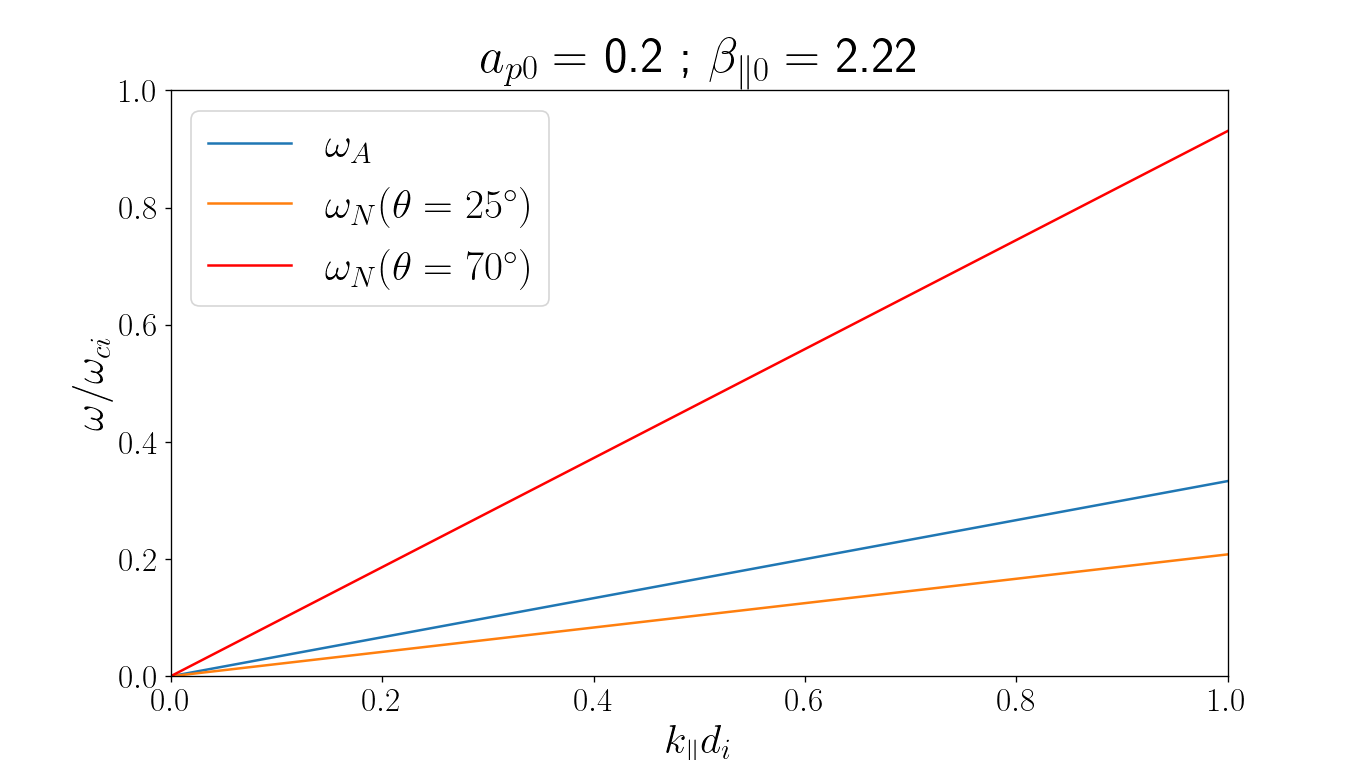
\includegraphics[width=0.8\linewidth,trim=2cm 0cm 3cm 1cm, clip=true]{./Part_2/images/lin_omega_k}
\caption{Mode d'Alfvén-firehose ($\omega_A$, bleu) et nouveau mode ($\omega_N $, orange pour $\theta = \ang{25}$ et rouge pour $\theta=\ang{70}$) normalisés par $\omega_{ci}$ la pulsation cyclotron des ions et représentés en fonction de $k_{\parallel}d_i$, avec $d_i = v_{A0}/ \omega_{ci}$, la longueur inertielle ionique. } 
\label{fig:lin_omega_k}
\end{figure}
On remarque que le nouveau mode peut être plus lent ou plus rapide que le mode d'Alfvén-firehose en fonction de $\theta$. Ce n'est pas montré ici, mais il peut aussi devenir instable quand le mode d'Alfvén-firehose est stable. Ils sont donc très différents. Ces observations, nous ont amené à faire une étude paramétrique en fonction de $\theta$ de la vitesse de phase et du taux de croissance/amortissement des instabilités. 

Au cours de cette étude, on a observé cinq comportements différents pour le nouveau mode suivant la valeur du couple  $\{\beta_{\parallel 0};a_{p0}\}$ . Ces comportements sont résumés sur la figure \ref{fig:lin_omega_theta} à travers cinq couples représentatifs. 
\begin{figure}[!ht]
 \centering
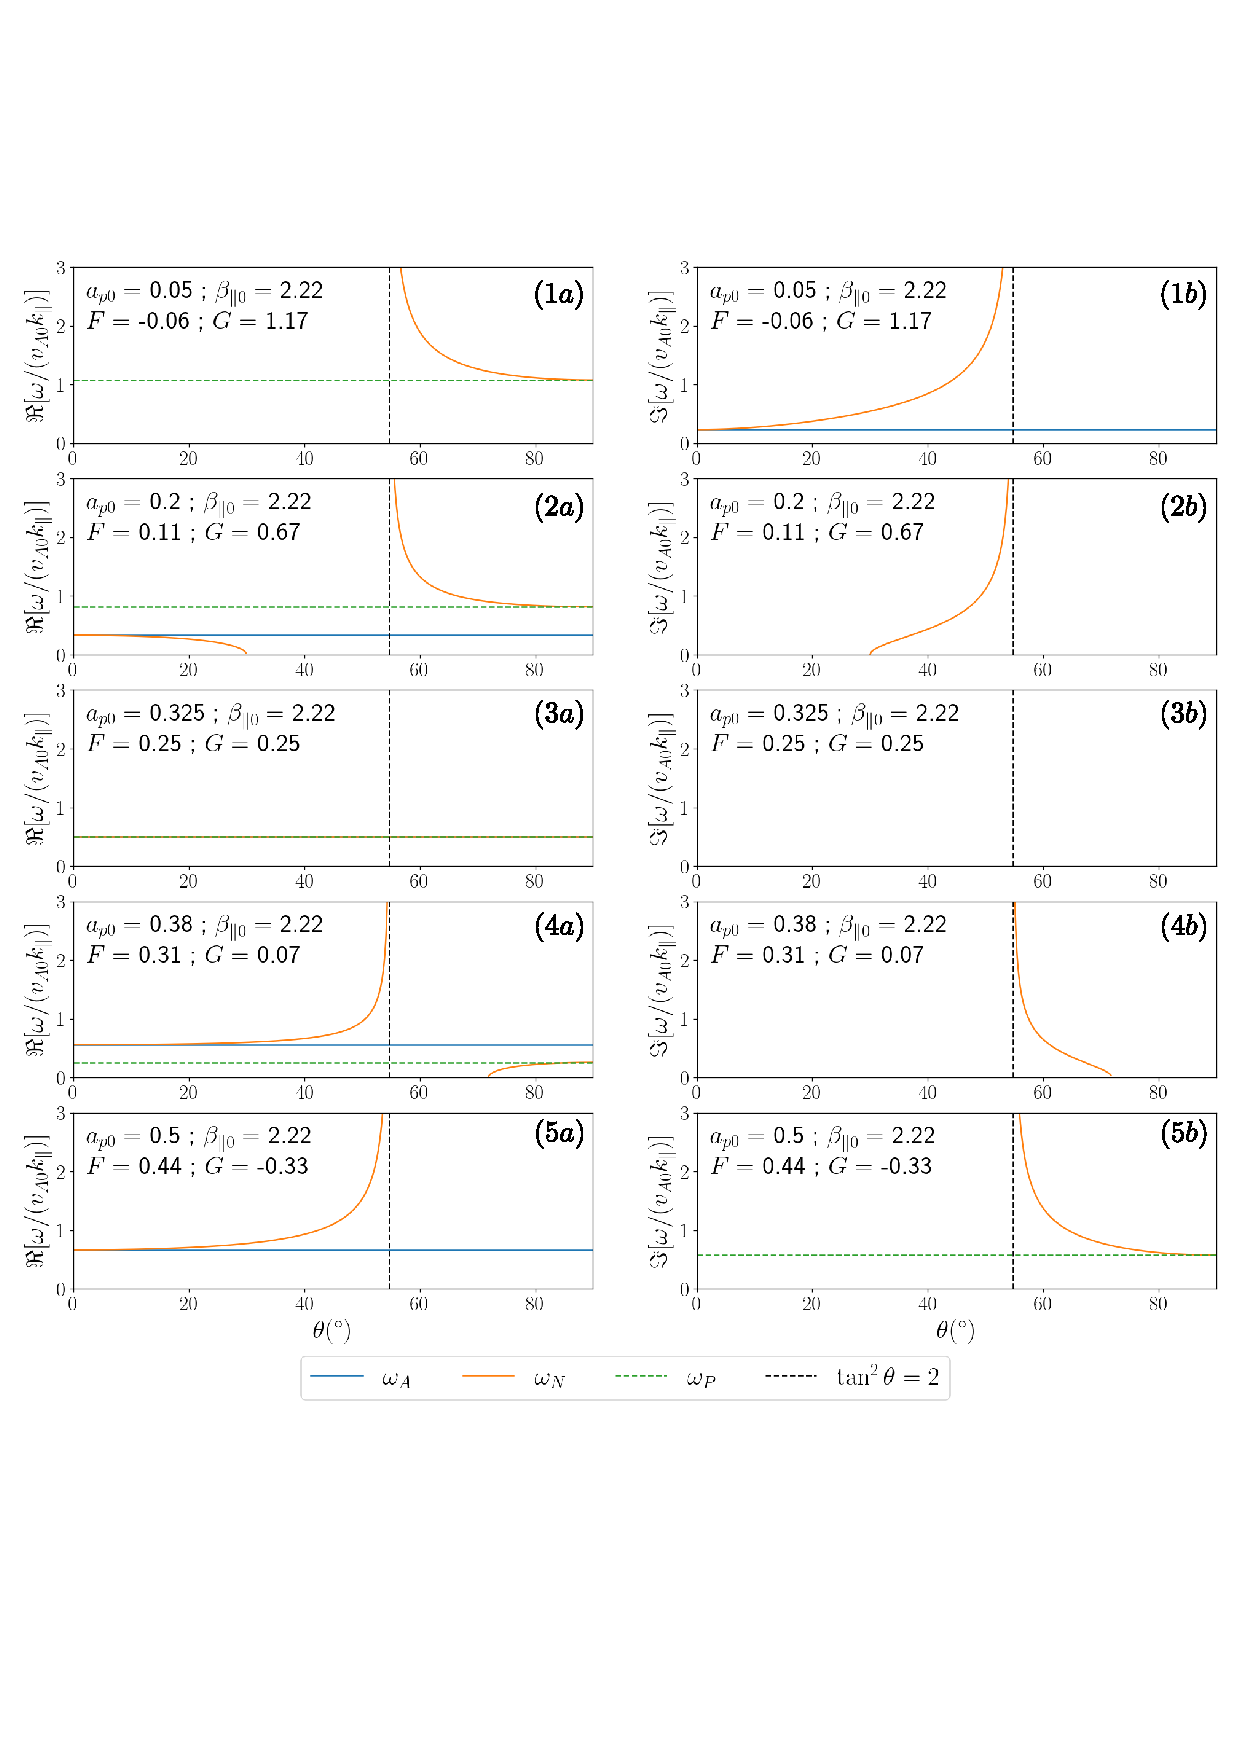
\includegraphics[width=\linewidth,trim=0.5cm 6cm 0cm 3cm, clip=true]{./Part_2/images/lin_omega_theta}
\caption{Vitesse de phase $\Re[\omega/(kv_{A0})]$ (colonne a) et taux de croissance des instabilités $\Im[\omega/(kv_{A0})]$ (colonne b) normalisées par $v_{A0}$ en fonction de l'angle $\theta$ pour le nouveau mode incompressible ($\omega_N$, orange) et pour le mode d'Alfvén ($\omega_A$, bleu). Des asymptotes sont tracées en lignes discontinues. En vert : mode asymptotique $\omega_P$. En noir : angle asymptotique $\theta_2$. Première ligne : couple (1) tel que $a_{p0} = 0.05$, $\beta_{\parallel 0} = 20/9 \Rightarrow$ instabilité firehose ($F<0$). Deuxième ligne : couple (2) tel que $a_{p0} = 0.2$, $\beta_{\parallel 0} = 20/9 $. Troisième ligne : couple (3) tel que $a_{p0} = 0.325$, $\beta_{\parallel 0} = 20/9 \Rightarrow$ seul cas stable pour tout $\theta$ ($F=G$). Quatrième ligne : couple (4) tel que $a_{p0} = 0.38$, $\beta_{\parallel 0} = 20/9  $. Cinquième ligne : couple (5) tel que $a_{p0} = 0.5$, $\beta_{\parallel 0} = 20/9  \Rightarrow$ instabilité pseudo-firehose perpendiculaire ($G<0$). Sauf graphique (3a) où tous les modes coincident, lorsque qu'un mode disparaît d'un graphique de la colonne a, il apparaît sur le graphique de la colonne b.}
\label{fig:lin_omega_theta}
\end{figure}
Sur l'ensemble de graphiques de la \figref{fig:lin_omega_theta} sont tracés en fonction de $\theta$, pour les cinq couples représentatifs et chaque mode, la partie réelle de $\omega$ normalisée par le mode d'Alfvén, $\Re[\omega/(k_{\parallel}v_{A0})]$ (colonne a) correspondant à sa vitesse de phase, ainsi que sa partie imaginaire ($\Im[\omega/(k_{\parallel}v_{A0})]$, colonne a), qui correspond au taux de croissance. $\omega$ étant ou réel ou purement imaginaire, ces graphiques sont complémentaires : si le mode est instable, il apparaîtra sur la colonne b, et s'il est stable sur la colonne a (à l'exception du graphique (3a) où les modes coîncident). Le caractère instable firehose du mode d'Alfvén (bleu) est ainsi retrouvé lorsque $F<0$ sur le graphique (1b). 

Le nouveau mode semble tendre asymptotiquement vers le mode d'Alfvén pour $\theta \sim \ang{0}$ et vers l'asymptote $\omega_P = \pm k_{\parallel}v_{A0} \sqrt{G}$ représentée par une ligne discontinue verte, pour $\theta \sim \ang{90}$. Une asymptote angulaire est aussi visible en un angle que l'on note $\theta_2$, on verra par la suite que cet angle est solution de $\tan^2 \theta = 2$. La stabilité du nouveau mode à une dépendance forte en $\theta$ : pour tout couple, il existe une gamme angulaire telle que le mode soit stable et, à l'exception du couple (3), une gamme telle que le mode est instable. 

On propose maintenant de démontrer les comportements identifiés pour le nouveau mode en fonction de $a_{p0}$ et $\beta_{\parallel 0}$. Au fil de cette analyse, on va construire le diagramme de la \figref{fig:lin_cases_update}. Les emplacements des différents couples présentés sur la \figref{fig:lin_omega_theta} sont indiqués par des croix rouges. 

\paragraph{Etude asymptotique angulaire : }Si $\theta \rightarrow \ang{0}$ ($k_{\parallel}\gg k_{\perp}$), alors $\frac{\omega^2_N}{v^2_{A0}k^2} \rightarrow F \cos^2 \theta$. La convergence vers le mode d'Alfvén-firehose du nouveau mode observée en $\theta \rightarrow \ang{0}$ sur la \figref{fig:lin_omega_theta} est ainsi vérifiée. Comme cette limite peut être stable ou instable en fonction du signe de $F$, on a représenté sur la \figref{fig:lin_cases_update}, la frontière $F=0$ en bleue et bleutée la zone où $F<0$. On retrouve dans ce comportement stable/instable l'instabilité firehose <<parallèle>> qui est présente par exemple pour le mode lent dans le cadre compressible. Le couple (1), tel que $F<0$, est un exemple instable : le nouveau mode et le mode d'Alfvén apparaîssent dans la colonne du taux de croissance (graphique (1b)). 

Si $\theta \rightarrow \ang{90}$ ($k_{\perp}\ll k_{\parallel} $), alors $\frac{\omega^2_N}{v^2_{A0}k^2} \rightarrow G \cos^2 \theta$. On retrouve l'asymptote $\omega_P$ et tracé en vert sur la \figref{fig:lin_omega_theta}. Il est instable si $G<0$. La comparaison de $G$ et $F$, qui ont la même structure à un facteur $3/2$ et un signe près, nous inspirant, on appellera cette instabilité <<instabilité pseudo-firehose perpendiculaire>>\footnote{Cette dénomination n'est proposée qu'à cause de la similarité des critères d'instabilités. Le comportement des quantités d'ordre 1 n'a pas été vérifié.}. Elle apparaît pour le couple (5) (graphique (5b)). Sur la \figref{fig:lin_cases_update}, on indique la frontière $G=0$ en vert et la zone où $G<0$ par une aire verte. 

{\bf Ainsi grâce à $F$ et $G$, on peut déduire qu'une instabilité pourra se développer dans le système pour tout couple $\{\beta_{\parallel 0};a_{p0}\}$ tel que $\frac{2}{3}>\frac{\beta_{\parallel 0}}{2}(1-a_{p0})$ (instabilité pseudo-firehose perpendiculaire, couple (5) et aire verte sur \figref{fig:lin_cases_update}) ou $\frac{\beta_{\parallel 0}}{2}(1-a_{p0})>1$ (instabilité firehose parallèle, couple (1) et aire bleue sur \figref{fig:lin_cases_update}).} Dans la zone intermédiaire (blanche sur la \figref{fig:lin_cases_update}), $G>0$ et $F>0$. 

\paragraph{Etude angulaire complète du nouveau mode : } Pour les angles $\theta$ plus obliques, le comportement de $\omega_N$ est plus difficile à établir, le signe de $\sin^2 \theta - 2 \cos^2 \theta$ venant compenser le signe de $G \sin^2 \theta - 2F \cos^2 \theta$. Une instabilité, entre l'instabilité firehose parallèle et l'instabilité pseudo-firehose perpendiculaire, pourra émerger. On la nommera <<instabilité pseudo-firehose oblique>>. Elle apparaît pour les couples (2) (graphique (2b)) et (4) (graphique (4b)). La condition d'instabilité est obtenue pour $F$ et $G$ tels que :  
\begin{eqnarray}
    (\tan^2 \theta - 2 )(G \tan^2 \theta - 2F ) &<& 0  .
\end{eqnarray}
$g(\theta) = (\tan^2 \theta - 2 )(G \tan^2 \theta - 2F )$ est une parabole présentant deux racines : 
\begin{itemize}
    \item $\tan^2 \theta = 2 $ en laquelle $\omega^2_N \rightarrow \infty$ (asymptote verticale indiquée en pointillés sur \figref{fig:lin_omega_theta}), on la note $\theta_2$,
    \item $\tan^2 \theta = 2\frac{F}{G}$ en laquelle $\omega^2_N \rightarrow 0$, on la note $\theta_{F/G}$.
\end{itemize}
La stabilité du nouveau mode dépendra donc de la position de $\theta$ par rapport à $\theta_2$ et $\theta_{F/G}$. 

Pour que le nouveau mode soit stable pour tout $\theta$, il faut $g(\theta)>0$ pour tout $\theta$. Cela n'est possible que si $F=G$, alors $g(\theta) = (\tan^2 \theta - 2 )^2 >0$. Dans ce cas, $\omega_N = \omega_A = \omega_P$. Sur la \figref{fig:lin_cases_update}, le critère $F=G$ est indiqué par la courbe noire et il est illustré par le couple (3) (graphiques (3a) et (3b)). {\bf Par conséquent, en fonction de $a_{p0}$ et $\beta_{\parallel 0}$, le nouveau mode sera stable pour tout $\theta$ si et seulement si $ \frac{\beta_{\parallel 0}}{2}(1-a_{p0}) = \frac{3}{4} $.}

$F=G$, $G=0$ et $F=0$ découpent le diagramme de la \figref{fig:lin_cases_update} en quatre zones que l'on va étudier séparément. 

Si $G<0$ (zone verte), alors $F>0$. Dans ce cas, $g(\theta) < 0$ si $\theta > \theta_2$. Cette situation est illustrée par le couple (5) (graphiques (5a) et (5b)), instable pour tout angle supérieur à $\theta_2$. On peut raccrocher à cette condition le cas $G=0$ puisque alors $F=1/3$, et la parabole sera négative si $\tan^2 \theta > 2$. Dans ces cas, on retrouve l'instabilité pseudo-firehose perpendiculaire découverte asymptotiquement si $\theta \rightarrow \ang{90}$. On peut maintenant compléter ses conditions d'existence qui deviennent : {\bf l'instabilité pseudo-firehose perpendiculaire peut se développer si $G<0$ pour tout angle $\theta > \theta_2$}.


Si $G>0$ et $F/G>1$ (zone blanche délimitée par les courbes verte et noire), $g(\theta) < 0$ si $2\frac{F}{G} > \tan^2 \theta > 2$. Cette situation est illustrée par le couple (4) (graphiques (4a) et (4b)). L'instabilité s'y développant est l'instabilité pseudo-firehose oblique. 


Si $G>0$ et $F/G<1$ (zone blanche délimitée par les courbes bleue et noire et zone bleue), $g(\theta) < 0$ si $2 > \tan^2 \theta > 2\frac{F}{G}$. {\bf Si $F<0$, l'instabilité firehose parallèle se développe pour tout angle  $\theta < \theta_2$. } Ce cas est illustré par le couple (1) (graphiques (1a) et (1b)). Si $F>0$, la situation est illustrée par le couple (2) (graphiques (2a) et (2b)). L'instabilité visible est encore une fois l'instabilité pseudo-firehose oblique. Sa condition d'apparition est donc : {\bf l'instabilité pseudo-firehose oblique peut se développer si $G>0$ et $F>0$ mais $G\neq F$, pour tout angle $\theta$ entre $\theta_2$ et $\theta_{F/G}$}. 

\begin{figure}[!ht]
 \centering
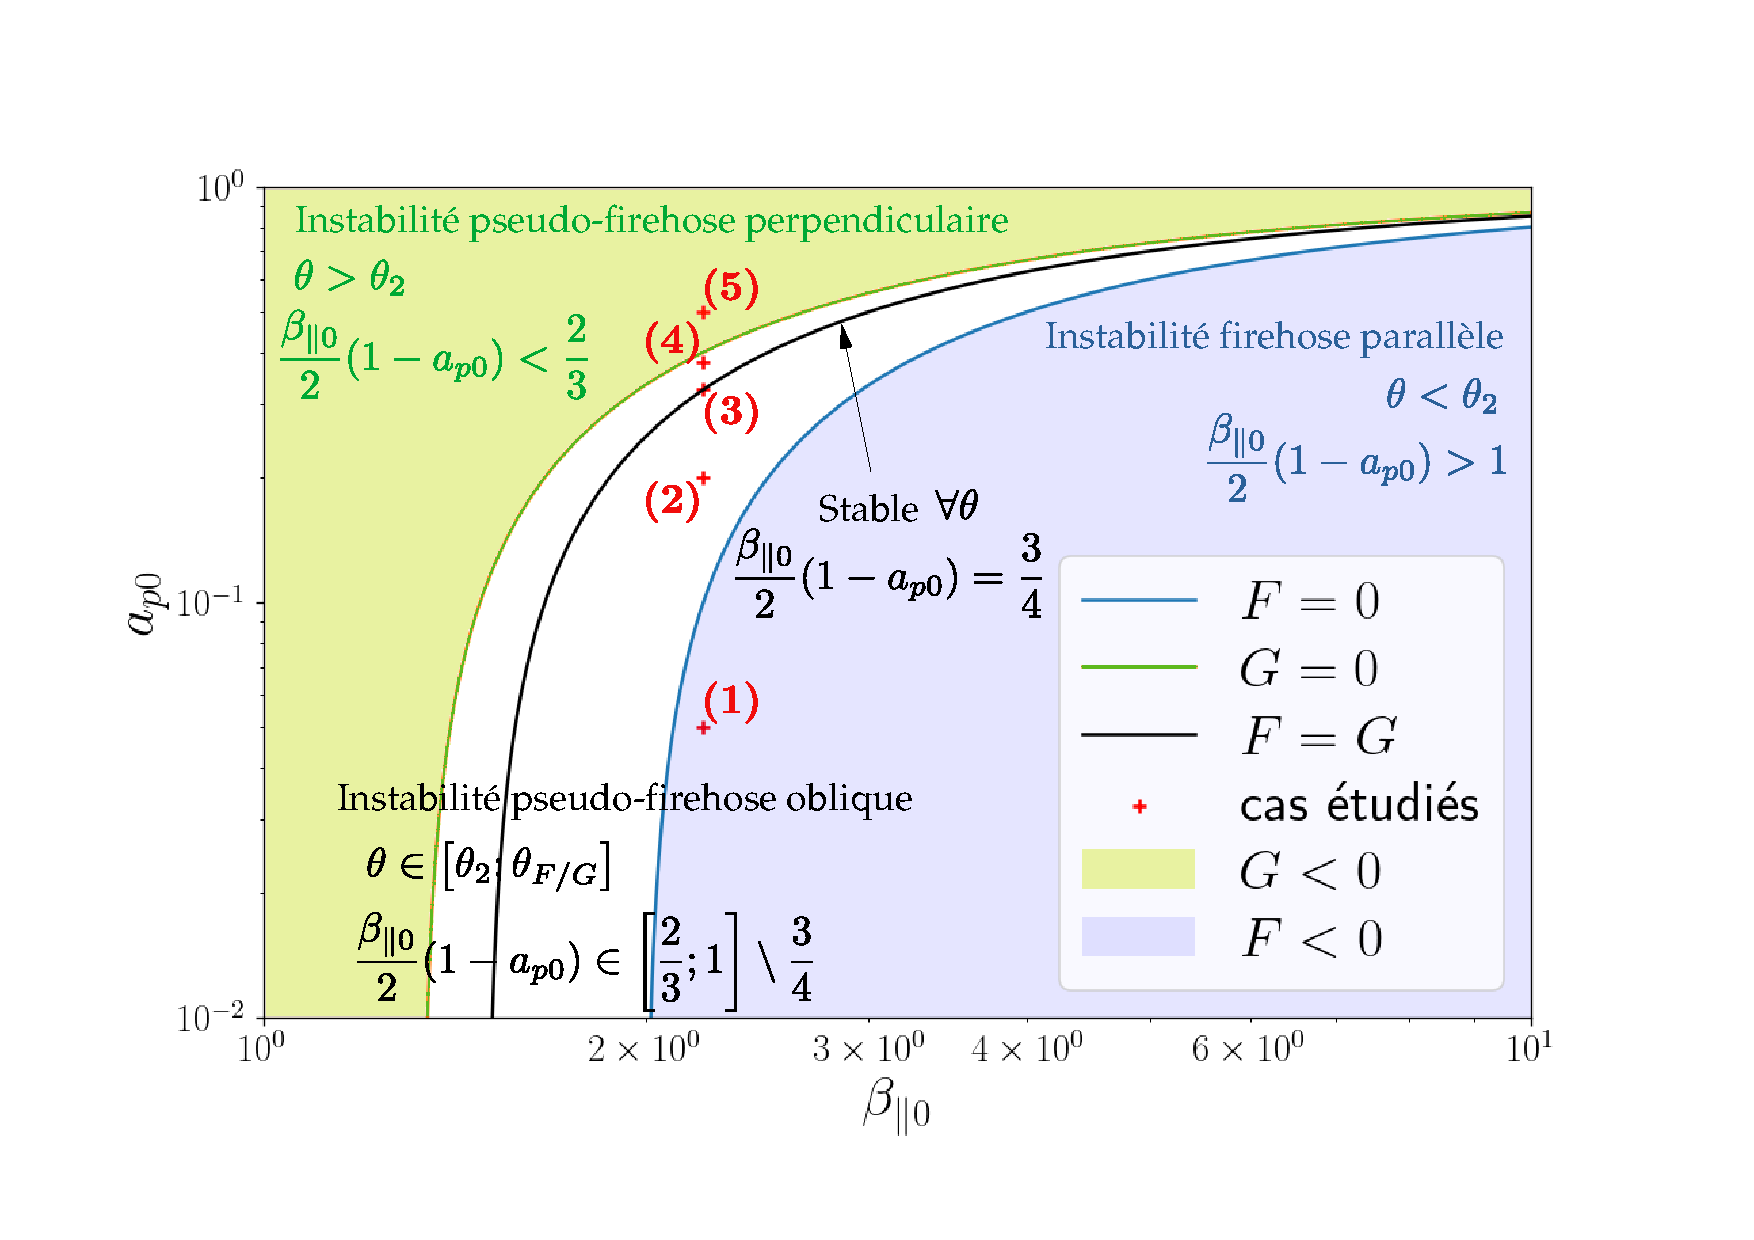
\includegraphics[width=1\linewidth,trim=2cm 1cm 3cm 2cm, clip=true]{./Part_2/images/diag_cas}
\caption{Diagramme $a_{p0}-\beta_{\parallel 0}$ résumant l'étude du nouveau mode. Croix rouges : couples $\{\beta_{\parallel 0};a_{p0}\}$ sélectionnés pour l'étude paramétrique de la \figref{fig:lin_omega_theta}. Frontière d'instabilités firehose $F=0$ (bleu) et zone instable ($F<0$, bleue) associée. Frontière d'instabilités pseudo-firehose perpendiculaire $G=0$ (verte) et zone instable ($G<0$, verte) associée. Ligne noire : ensemble des couples $\{\beta_{\parallel 0};a_{p0}\}$ stables pour tout angle $\theta$ paramétrisé par  $F=G$. Zone blanche : instabilité pseudo-firehose oblique. }
\label{fig:lin_cases_update}
\end{figure}


La zone de stabilité de ce nouveau mode en fonction des paramètres $\beta_{\parallel 0}$ et $a_{p0}$ est donc quasi-inexistante. Un résumé de l'ensemble des éléments de cette analyse est donnée sur la \figref{fig:lin_cases_update}. Sachant que la problématique principale de ce travail se place dans le cadre compressible, l'exploitation de ce modèle incompressible n'a pas été engagée mais il fera l'objet d'un nouveau papier en préparation [\cite{simon_article_2023}]. 


% \section{Limite incompressible du modèle \ac{CGL}}\label{sec-224}

% Dans le cas \ac{MHD} compressible avec pression isotrope, le mode pseudo-alfvénique apparaît comme une limite incompressible des modes compressibles magnétosonores. Similairement, on s'est demandé si l'on pouvait retrouver une trace du nouveau mode dans la limite incompressible du modèle \ac{CGL} linéaire. 

% Dans le cas linéaire, le modèle \ac{CGL} donne l'équation de dispersion \eqref{eq:lin_cpg_eqdis} que l'on va simplement noter $\overline{\boldsymbol{M}} \boldsymbol{v}_1 = 0$. Avec la contrainte incompressible $\nabla \cdot \boldsymbol{v}_1 = 0$, on peut écrire $\boldsymbol{v}_1$ sous la forme d'un potentiel vecteur $\boldsymbol{\Omega}$ : $\boldsymbol{v}_1 = \nabla \times \boldsymbol{\Omega} = \overline{\boldsymbol{N}}\boldsymbol{\Omega}$ avec $\overline{\boldsymbol{N}} = i \boldsymbol{k} \times \overline{\boldsymbol{I}} = i \begin{pmatrix} 0&-k_{\parallel}&0\\k_{\parallel}&0&-k_{\perp}\\ 0&k_{\perp}&0 \end{pmatrix} $. Le modèle \ac{CGL} linéaire surcontraint via l'incompressibilité s'exprime alors à travers l'équation de dispersion : $\overline{\boldsymbol{M}}  \overline{\boldsymbol{N}} \boldsymbol{\Omega}=0$ avec 
% \begin{equation}
%     \overline{\boldsymbol{M}} \overline{\boldsymbol{N}} = \begin{pmatrix}
% \label{eq:lin_cpginc_eqdis}  0&  -k_{\parallel}(\frac{\omega^2-\omega^2_A}{v^2_{A0}k^2_{\parallel}} -  (\frac{\beta_{\parallel 0}}{2} a_{p0} +1 ) \frac{k^2_{\perp}}{k^2_{\parallel}})  & 0  \\
%     k_{\parallel} \frac{\omega^2 - \omega^2_A}{v^2_{A0}k^2_{\parallel}}  & 0 & - k_{\perp}\frac{\omega^2-\omega^2_A}{v^2_{A0}k^2_{\parallel}}\\
%       0  &k_{\perp}(\frac{\omega^2 }{ v^2_{A0}k^2_{\parallel}} -   \frac{\beta_{\parallel 0}}{2}  (3-a_{p0})) &0 
%     \end{pmatrix} ,
% \end{equation}
% où $\omega^2_A = - v^2_{A0}k^2_{\parallel} ( \frac{\beta_{\parallel 0}}{2} (1-a_{p0})-1)$ correspond au mode d'Alfvén-firehose incompressible. On remarque que ce mode est solution si $\Omega_y = 0$, c'est-à-dire pour une polarisation de la vitesse orientée suivant $(0,1,0)$. 

% On a vu dans la section \ref{sec-222} que le nouveau mode est polarisé suivant $(\cos \theta,0,-\sin \theta)$.  Si l'on impose cette polarisation dans $\Omega$ on obtient $\Omega_y \neq 0$. Dans ce cas l'équation de dispersion peut alors s'écrire sous la forme du système :
% \begin{eqnarray}
%     \label{eq:lin_cglinc_1} k_{\parallel}(\omega^2-\omega^2_A - v^2_{A0}  (\frac{\beta_{\parallel 0}}{2} a_{p0} +1 ) k^2_{\perp}) &=& 0 ,\\
%      \label{eq:lin_cglinc_2} k_{\perp}(\omega^2  - v^2_{A0}   \frac{\beta_{\parallel 0}}{2}  (3-a_{p0}) k^2_{\parallel})&=& 0 ,\\
%      \label{eq:lin_cglinc_3} k_{\parallel}\Omega_x - k_{\perp}\Omega_z&=&0 .
% \end{eqnarray}
% On va étudier ce système en fonction de l'angle $\theta$ de propagation : 
% \begin{itemize}
%     \item $\theta = \ang{0} \Rightarrow k_{\perp} = 0$ et on suppose  $ k_{\parallel} \neq 0$, alors $\omega^2 =\omega^2_A$ et $\Omega_x =0$. On retrouve le mode firehose parallèle associé à un champ de vitesse sera polarisé suivant $(1,0,0)$.
%     \item $\theta = \ang{90} \Rightarrow k_{\parallel}  = 0$ et on suppose  $k_{\perp} \neq 0$, alors $\omega^2 =0$ et $\Omega_z =0$. On obtient un mode qui ne se propage pas et un champ de vitesse polarisé suivant $(0,0,1)$.
%     \item Si $ k_{\parallel} \neq 0$ et $k_{\perp} \neq 0$, alors $\omega^2  = v^2_{A0}   \frac{\beta_{\parallel 0}}{2}  (3-a_{p0})k^2_{\parallel}$ et $\theta$ doit vérifier $\tan^2 \theta  =\frac{2(\beta_{\parallel 0}(2-a_{p0})-1)}{\beta_{\parallel 0} a_{p0}+2}$.
% \end{itemize}
% Après quelques manipulations de $\omega^2  = v^2_{A0}   \frac{\beta_{\parallel 0}}{2}  (3-a_{p0})k^2_{\parallel}$ et de la condition $\tan^2 \theta  =\frac{2(\beta_{\parallel 0}(2-a_{p0})-1)}{\beta_{\parallel 0} a_{p0}+2}$, il est possible de faire ressortir la relation de dispersion du nouveau mode. 

% On remarque qu'appliquer la contrainte incompressible sur le modèle \ac{CGL} revient à chercher la limite telle que $p_{\parallel}$ ou $p_{\perp}$ respecte leur équation individuelle dans le modèle incompressible gyrotrope. En fait, la limite incompressible du modèle \ac{CGL} correspond à l'intersection des solutions des modèles incompressible gyrotrope défini avec la trace de la pression, incompressible gyrotrope défini avec l'équation sur $p_{\parallel}$ et incompressible gyrotrope défini avec l'équation sur $p_{\perp}$. Dans chacun de ces modèles, le mode d'Alfvén-firehose sera accompagné d'un nouveau mode dont l'expression dépend du choix de la fermeture sur la pression. Mais tous seront polarisé tel que $(\cos \theta,0,-\sin \theta)$ et peuvent être retrouvés dans le mode surcontraint du modèle \ac{CGL}. 

\newpage
\section{Synthèse : Limite incompressible et pistes d'étude}
\label{synt-22}

\fcolorbox{red}{white}{\begin{minipage}[c]{\linewidth}
\paragraph{Limite incompressible de la loi exacte avec pression tensorielle et cas gyrotrope :}
\begin{eqnarray}
    \label{eq:synth_turbinc_pgen} - 4(\varepsilon - \varepsilon_{PP98}) &=& -2 \left< \delta (\overline{\boldsymbol{P}} - p \overline{\boldsymbol{I}}):\delta (\nabla \boldsymbol{v}) \right> = -2 \left< \delta \overline{\boldsymbol{\Pi}} :\delta (\nabla \boldsymbol{v}) \right>,\\
\label{eq:synth_turbinc_pgyr} - 4(\varepsilon - \varepsilon_{PP98}) &=& -2 \left< \delta ((p_{\parallel} - p_{\perp})(\boldsymbol{b}\boldsymbol{b} -\frac{1}{3} \overline{\boldsymbol{I}})):\delta (\nabla \boldsymbol{v}) \right>.
\end{eqnarray}
$\Rightarrow$ Questionne l'existence d'un modèle incompressible gyrotrope. 


\paragraph{Modèle incompressible avec pression gyrotrope proposé compatible avec la loi exacte : }
\begin{eqnarray}
\label{eq:synth_incg_v} \partial_t  \boldsymbol{v} + \nabla \cdot (\boldsymbol{v}\boldsymbol{v} - \boldsymbol{v_A}\boldsymbol{v_A} + \frac{1}{\rho_0} \overline{\boldsymbol{P_*}})  &=& 0  ,\\
\label{eq:synth_incg_p} \partial_t p + \nabla \cdot (p \boldsymbol{v} ) + \frac{2}{3} \overline{\boldsymbol{\Pi}} : \nabla \boldsymbol{v}   &=& 0 ,  \\
\label{eq:synth_incg_b} \partial_t \boldsymbol{v_A} -  \nabla \cdot (\boldsymbol{v_A}\boldsymbol{v} - \boldsymbol{v}\boldsymbol{v_A}) &=& 0 ,\\
 \text{avec } \quad \overline{\boldsymbol{P_*}} = (p+p_m) \overline{\boldsymbol{I}} + \overline{\boldsymbol{\Pi}}, \quad p_m = \frac{\rho_0 | \boldsymbol{v_A}|^2}{2}, \quad p = \frac{1}{3} (2 p_{\perp} + p_{\parallel} ), &&  \nonumber\\ \overline{\boldsymbol{\Pi}} = (p_{\parallel} - p_{\perp})(\boldsymbol{b}\boldsymbol{b} - \frac{1}{3} \overline{\boldsymbol{I}}),  \quad \boldsymbol{b} = \frac{\boldsymbol{v_A}}{|\boldsymbol{v_A}|}, \quad \text{et} \quad \nabla \cdot \boldsymbol{v} &=&  0.  \nonumber
\end{eqnarray}

\paragraph{Etude linéaire du modèle proposé : }
\begin{itemize}
    \item Mode d'Alfvén incompressible polarisé suivant $(0,1,0)$ :
\begin{eqnarray}
\label{eq:synth_lininc_disp1}    
  \frac{\omega^2}{v^2_{A0}k^2_{\parallel}} + \frac{\beta_{\parallel 0}}{2}(1-a_{p0})-1  &=&0,\\
\text{Instabilité firehose : } \frac{\beta_{\parallel 0}}{2}(1-a_{p0})-1 &>&0 .
\end{eqnarray} 
    \item Nouveau mode polarisé suivant $(1,0,- \tan \theta)$ : (voir la \figref{fig:lin_cases_update})
\begin{eqnarray}
\label{eq:synth_lininc_disp2}    
  \frac{\omega^2}{v^2_{A0}k^2_{\parallel}} - \frac{2(\frac{\beta_{\parallel 0}}{2}(1-a_{p0})-1)\cos^2 \theta 
  +  ( 3\frac{\beta_{\parallel 0}}{2}(1-a_{p0}) - 2) \sin^2 \theta}{\sin^2 \theta-2\cos^2 \theta}  =0. && \\
\text{Critère d'instabilité pseudo-firehose : }  \frac{\beta_{\parallel 0}}{2}(1-a_{p0}) \neq \frac{3}{4}. && 
\end{eqnarray} 
\end{itemize}

% \paragraph{\\Limite incompressible du modèle \ac{CGL} :}
% \begin{itemize}
%     \item Survie du mode d'Alfvén-firehose $\Rightarrow$ Solution non-linéaire, pendant gyrotrope du mode d'Alfvén non linéaire ?
%     \item Apparition d'un mode surcontraint correspondant au nouveau mode incompressible.
% \end{itemize}

Les résultats obtenus ici à propos du nouveau modèle semble prometteur et feront l'objet d'une publication future. 
\end{minipage}}

\chapter{Relaxer l'approximation \ac{MHD} et aller vers le bi-fluide}
\renewcommand\partie{\Partie\ Chapitre \thechapter}
\label{ch-23}
\bigskip
\minitoc  

Dans les chapitres précédents, l'équation d'induction \eqref{eq:model_cpg_b} était celle de l'approximation \ac{MHD}. Dans ce chapitre, nous allons relaxer les hypothèses sur cette équation en prenant d'abord en compte le terme de \acs{Hall} (section \ref{sec-231}). Dans la section \ref{sec-233}, nous dériverons une correction à la loi exacte associée à chaque niveau d'approximation de la loi d'Ohm en partant du modèle bi-fluide. Enfin dans la section \ref{sec-232}, nous nous intéresserons au modèle gyrotrope utilisé dans les simulations étudiées dans la Partie \ref{part_3} : un modèle \acs{LFCGLHPe} (avec la fermeture \ac{LF} gyrotrope telle que $\overline{\overline{\boldsymbol{q}}} \neq 0$) prenant en compte la pression électronique dans la loi d'Ohm avec différentes fermetures (isotherme et gyrotrope). 

\section{La \acs{MHDH}}
\label{sec-231}

Comme on l'a vu dans le Chapitre \ref{ch-02}, le terme de \acs{Hall} doit être pris en compte dans l'équation d'induction si l'on regarde des échelles proches de la longueur inertielle des ions, ou des fréquences proches de la fréquence cyclotron des ions. Par conséquent, la loi exacte obtenue avec une loi d'Ohm \ac{MHD} perdra en validité près de ces échelles. Afin de tirer la description de la cascade dans ce domaine ionique, on doit donc calculer une correction à partir du terme de \acs{Hall}. Diverses formulations existent pour cette contribution dans le cas des modèles dépendant d'une pression isotrope mais que devient-elle dans le cadre d'une fermeture avec pression tensorielle ? 

En prenant en compte le terme de \acs{Hall}, l'équation d'induction devient : 
\begin{equation}
\label{eq:model_hall1} \partial_t \boldsymbol{v_A}  =   \nabla \cdot \left(\boldsymbol{v_A}\boldsymbol{u} - \boldsymbol{u}\boldsymbol{v_A}\right) -  \boldsymbol{u}  \nabla \cdot \boldsymbol{v_A} +  \frac{\boldsymbol{v_A}}{2}  \nabla \cdot \boldsymbol{u} - \frac{\lambda_i}{ \sqrt{\rho} } \nabla \times \left(\frac{\boldsymbol{j}}{\sqrt{\rho}}  \times \boldsymbol{v_A}\right) ,
\end{equation}
avec $\lambda_i = m_i/|q_e|$, constante analysée dans le chapitre \ref{ch-02} de l'Introduction,  $\boldsymbol{j} = \frac{1}{\sqrt{\mu_0}} \nabla \times \left(\sqrt{\rho}\boldsymbol{v_A}\right)$, la densité de courant et $\mu_0$ la perméabilité du vide. 

Puisque $\sqrt{\rho} \boldsymbol{v_A} \cdot \nabla \times \left(\frac{\boldsymbol{j}}{\sqrt{\rho}}  \times \boldsymbol{v_A}\right) = \nabla \cdot \left(\left(\boldsymbol{j}  \times \boldsymbol{v_A}\right)\times \boldsymbol{v_A} \right)$, l'équation d'énergie magnétique \eqref{eq:model_cpi_m} devient :
\begin{equation}
  \label{eq:model_cpgh_m}   \partial_t E_m  +\nabla   \cdot  \left(E_m\boldsymbol{v}+ \lambda_i \left(\boldsymbol{j}  \times \boldsymbol{v_A}\right)\times \boldsymbol{v_A} \right)  = \rho  \boldsymbol{v_A}\boldsymbol{v_A}  : \nabla \boldsymbol{v}- p_m  \nabla \cdot \boldsymbol{v} .
\end{equation}
Cette correction n'ajoute qu'un terme de type flux au bilan énergétique et n'impactera pas l'équation d'énergie interne. De plus, le terme de \acs{Hall} ne dépend pas du tenseur de pression. Par conséquent, elle n'influera pas littéralement sur les contributions du tenseur de pression et de l'énergie interne dans la loi exacte. Il faudra tout de même faire attention à ne pas utiliser les formes conservatives des pressions parallèle et perpendiculaire \acs{CGL} \eqref{eq:model_cpg_biadiab} qui ne sont valables que dans le cas \ac{MHD}, l'équation d'induction \ac{MHD} étant utilisée pour les obtenir.

En notant génériquement $\varepsilon_{mhd}$ le taux de cascade compressible obtenu avec un modèle dans lequel le terme de \acs{Hall} est négligé et $\varepsilon_{hall}$ la correction \acs{Hall}, le nouveau taux de cascade sera $\varepsilon = \varepsilon_{mhd} + \varepsilon_{hall}$ avec  :
%\begin{eqnarray}
\begin{equation}
\label{eq:corr_hall} \boxed{
\begin{array}{lcl}
    -4\varepsilon_{hall} &=& \lambda_i\nabla_{\boldsymbol{\ell}} \cdot \left< \left(\boldsymbol{j}  \times \boldsymbol{v_A}+ \boldsymbol{j'}  \times \boldsymbol{v'_A}\right)\times \delta \boldsymbol{v_A} - \delta \left(\frac{\boldsymbol{j}}{\rho}  \times \boldsymbol{v_A}\right)\times \left(\rho \boldsymbol{v_A}+ \rho' \boldsymbol{v'_A}\right)\right> \\
    &+& \frac{\lambda_i}{2} \left< \left(\rho' \boldsymbol{v'_A} \cdot \delta \boldsymbol{v_A}- \delta \left(\rho \boldsymbol{v_A}\right) \cdot \boldsymbol{v'_A} \right)\nabla \cdot \left(\frac{\boldsymbol{j}}{\rho}\right) - \left(\rho \boldsymbol{v_A} \cdot \delta \boldsymbol{v_A}- \delta \left(\rho \boldsymbol{v_A}\right) \cdot \boldsymbol{v_A} \right) \nabla' \cdot \left(\frac{\boldsymbol{j'}}{\rho'}\right)\right> \\%\nonumber 
    &-& \lambda_i \left< \left(\rho' \boldsymbol{v'_A} \cdot \delta \left(\frac{\boldsymbol{j}}{\rho}\right)- \boldsymbol{v'_A} \cdot \delta \boldsymbol{j}  \right)\nabla \cdot \boldsymbol{v_A} - \left(\rho \boldsymbol{v_A} \cdot \delta \left(\frac{\boldsymbol{j}}{\rho}\right)- \boldsymbol{v_A} \cdot \delta \boldsymbol{j}  \right)\nabla' \cdot \boldsymbol{v'_A}\right> .
   \end{array}}
\end{equation} 
%\end{eqnarray}
Ce résultat est une adaptation à nos notations du résultat obtenu par \cite{andres_exact_2018} qui utilise la même fonction de corrélations de l'énergie magnétique, $\mathcal{R}_{m} = \frac{1}{4}\left<\left(\rho'+\rho\right)\boldsymbol{v'_A} \cdot \boldsymbol{v_A}\right>$, que nous.

Dans le cas incompressible avec pression isotrope, diverses formes de $\varepsilon_{hall}$ existent et ont été comparées par \cite{ferrand_exact_2019}. 
On retiendra la forme qu'ils ont dérivée et qui peut être retrouvée en prenant la limite incompressible de la correction \eqref{eq:corr_hall} :
\begin{equation}
\label{eq:corr_hallinc} \boxed{
\begin{array}{lcl}
    -4 \varepsilon_{hall} &{}_{\overrightarrow{\rho = \rho_0}}&  -\frac{\lambda_i}{2} \nabla_{\boldsymbol{\ell}} \cdot \left<\delta \boldsymbol{v_A} \cdot \delta \boldsymbol{v_A}\delta \boldsymbol{j} - 2 \delta \boldsymbol{v_A} \cdot \delta \boldsymbol{j} \delta \boldsymbol{v_A}\right> . %\nonumber \\ 
   \end{array}}
\end{equation} 
Similairement à la correction compressible, cette correction est applicable à notre loi incompressible avec pression gyrotrope. 

Linéairement, le terme de \acs{Hall} va adapter les modes \ac{MHD} et \acs{CGL} afin d'y faire apparaître des corrections proches de la fréquence cyclotron ionique $\omega_{ci} = \frac{B_0}{\lambda_i}$. Des modes whistler (sifflants) et cyclotron ionique vont émerger. Pour plus de détails, se référer à la dérivation effectuée par \cite{hunana_introductory_2019}. On notera que plus l'angle de propagation sera oblique par rapport à $\boldsymbol{b_0}$ et plus la correction \acs{Hall} à la relation de dispersion sera affaiblie. En terme d'instabilité, l'instabilité firehose sera quelque peu stabilisée. En effet, le critère d'instabilité devient $\frac{\beta_{\parallel 0}}{2}(1- a_{p0} ) > 1+\frac{k_{\parallel}^2 v^2_{A0}}{4\omega^2_{ci}}$. Par conséquent, la zone de stabilité du cadran $a_{p0}<1$ dans le diagramme $a_{p0}-\beta_{\parallel0}$ (\figref{fig:diag_cgl}) sera élargie : en $a_{p0}=0$, le critère rejoindra $\beta_{\parallel 0} = 2+\frac{k_{\parallel}^2 v^2_{A0}}{2\omega^2_{ci}}$ qui est supérieur au $\beta_{\parallel 0} = 2$ obtenu dans le cas \acs{CGL}. Le critère miroir ne sera quant à lui pas modifié. 

\section{Le modèle bi-fluide}
\label{sec-233}

Par curiosité, on s'est demandé à quoi ressemblerait la loi exacte si l'on prenait en compte l'ensemble de la loi d'Ohm généralisée \eqref{eq:ohm} dans l'équation d'induction. Au lieu d'attaquer ce problème en relaxant petit à petit les approximations appliquées sur la loi d'Ohm, j'ai choisi de partir du modèle bi-fluide puis d'y prendre en compte la quasi-neutralité et de l'exprimer en fonction des grandeurs mono-fluide et enfin d'y injecter la loi d'Ohm généralisée. Il est ensuite possible de faire tendre la loi exacte obtenue vers différents régimes similairement au travail effectué par \cite{banerjee_scale--scale_2020}. Contrairement à \cite{banerjee_scale--scale_2020} proposant une loi dérivée avec un modèle bi-fluide fermé polytropiquement et similairement à la dérivation effectuée dans le Chapitre \ref{ch-21}, on considèrera des pressions tensorielles et les équations d'énergie interne associée à chaque espèce en négligeant les flux de chaleur. Pour alléger un peu le calcul, on ne fait pas apparaître non plus les termes de forçage et dissipation.

La fonction de corrélation pour l'énergie électromagnétique sera choisie au plus près de celle utilisée jusqu'à présent c'est-à-dire $\left<\rho \boldsymbol{v_A}\cdot \boldsymbol{v'_A}\right>$.

Les équations bi-fluides utilisées
%non relativiste\footnote{L'hypothèse non-relativiste nous permet de négliger $q_r n_r \boldsymbol{E}$ devant $q_r n_r \boldsymbol{v_r} \times \boldsymbol{B}$  dans \eqref{eq:model_bi_v} (on l'y indique entre parenthèse car on en aura besoin dans la loi d'Ohm généralisée) et $\varepsilon_0 \mu_0 \partial_t \boldsymbol{E}$ devant $\nabla \times \boldsymbol{B}$ dans \eqref{eq:model_bi_EB3}.} utilisée avec $r = i,e$ 
sont : 
\begin{eqnarray}
  \label{eq:model_bi_r} \partial_t \rho_{\alpha} + \nabla \cdot \left(\rho_{\alpha} \boldsymbol{v_{\alpha}}\right) &=& 0 ,\\
  \label{eq:model_bi_v} \partial_t \left(\rho_{\alpha} \boldsymbol{v_{\alpha}}\right) + \nabla \cdot \left(\rho_{\alpha} \boldsymbol{v_{\alpha}}\boldsymbol{v_{\alpha}} + \overline{\boldsymbol{P_{\alpha}}}\right) - Q_{\alpha} \boldsymbol{E} - \boldsymbol{j_{\alpha}} \times \boldsymbol{B} &=& 0 ,\\
  \label{eq:model_bi_u} \partial_t  u_{\alpha} + \boldsymbol{v_{\alpha}} \cdot \nabla u_{\alpha}   + \frac{1}{\rho_{\alpha}} \overline{\boldsymbol{P_{\alpha}}} : \nabla \boldsymbol{v_{\alpha}}   &=& 0 ,\\
\label{eq:model_bi_EB1} \nabla \cdot \boldsymbol{E} =  \frac{Q}{\varepsilon_0} \qquad \nabla \times \boldsymbol{B} = \mu_0  \boldsymbol{j} + \mu_0 \varepsilon_0 \partial_t \boldsymbol{E} \qquad \nabla \cdot \boldsymbol{B} &=& 0 , \\
\label{eq:model_bi_EB4}\partial_t \boldsymbol{B} + \nabla \times \boldsymbol{E}   &=&  0 ,
\end{eqnarray}
avec $Q = \sum_{\alpha} Q_{\alpha} =  \sum_{\alpha} q_{\alpha} n_{\alpha}$, $\boldsymbol{j} = \sum_{\alpha} \boldsymbol{j_{\alpha}} = \sum_{\alpha} q_{\alpha} n_{\alpha} \boldsymbol{v_{\alpha}}  $. 

Ces équations contiennent beaucoup de quantités constantes : $m_{\alpha}$ dans $\rho_{\alpha}$, $q_{\alpha}$ pour chaque espèce, $ \mu_0$, $\varepsilon_0$. Afin de réduire ce nombre de constantes qui viendront alourdir les calculs et de faire ressortir des constantes caractéristiques du plasma, nous allons normaliser les équations\footnote{Cela n'a pas été entreprit dans les modèles mono-fluides utilisés précédemment, parce qu'en \acs{MHD} et \ac{MHDH}, les seules échelles apparaissant sont celles des ions (puisque $m_e \ll m_i$).}. 
Ces constantes caractéristiques sont le rapport de masse $\mu = \frac{m_e}{m_i+m_e} \simeq \frac{m_e}{m_i}$ puisque $m_e \ll m_i$, qui permet d'accéder facilement aux régimes \ac{MHD} ($\mu \rightarrow 0$) ou \ac{MHD} électronique (\acs{EMHD}, $\mu \rightarrow 1$) et une longueur inertielle sans dimension $\lambda_i = \frac{\sqrt{m_i+m_e}}{L_0 \sqrt{\mu_0 n_0 e^2}} \simeq \frac{\sqrt{m_i}}{L_0 \sqrt{\mu_0 n_0 e^2}}$ que l'on note $\lambda_i$ pour faciliter les comparaisons avec les résultats dimensionnés. Les vitesses seront normalisées par la vitesse de la lumière dans le vide $c$, et l'on note les quantités de références :
\begin{itemize}
    \item Longueur : $L_0$,
    \item Temps : $t_0 = \frac{L_0}{c}$,
    \item Vitesse : $V_0 = c$,
    \item Densité de particule : $n_0$,
    \item Champ magnétique : $B_0 = c \sqrt{\mu_0 n_0 (m_i+m_e)}$,
    \item Champ électrique : $E_0 = c B_0$,
    \item Pression : $P_0 = (m_i+m_e)n_0 c^2$.
\end{itemize}
On pourrait noter les quantités sans dimension avec un << $\tilde{}$ >>, par exemple $\tilde{\boldsymbol{v_i}} = \boldsymbol{v_i}/V_0$, etc. Cependant, dans la suite de cette section, on ne fera pas apparaître les << $\tilde{}$ >> afin d'alléger les notations.

Le système sans dimension s'écrit donc :
\begin{eqnarray}
  \label{eq:model_adbi_ri} \partial_t n_i + \nabla \cdot \left(n_i \boldsymbol{v_i}\right) &=& 0, \\
  \label{eq:model_adbi_re} \partial_t n_e + \nabla \cdot \left(n_e \boldsymbol{v_e}\right) &=& 0, \\
  \label{eq:model_adbi_vi} \partial_t  \boldsymbol{v_i} +\boldsymbol{v_i} \cdot \nabla \boldsymbol{v_i} + \frac{1}{(1-\mu) n_i} \nabla \cdot \overline{\boldsymbol{P_i}} - \frac{1}{(1-\mu)\lambda_i} \boldsymbol{E} - \frac{1}{(1-\mu)\lambda_i}  \boldsymbol{v_i} \times \boldsymbol{B} &=& 0 ,\\
  \label{eq:model_adbi_ve}  \partial_t  \boldsymbol{v_e} +\boldsymbol{v_e} \cdot \nabla \boldsymbol{v_e} + \frac{1}{\mu n_e} \nabla \cdot \overline{\boldsymbol{P_e}} + \frac{1}{\mu \lambda_i}  \boldsymbol{E} + \frac{1}{\mu \lambda_i} \boldsymbol{v_e} \times \boldsymbol{B} &=& 0 ,\\
  \label{eq:model_adbi_ui} \partial_t  u_i + \boldsymbol{v_i} \cdot \nabla u_i   + \frac{1}{(1-\mu)n_i} \overline{\boldsymbol{P_i}} : \nabla \boldsymbol{v_i}   &=& 0 ,\\
\label{eq:model_adbi_ue} \partial_t  u_e + \boldsymbol{v_e} \cdot \nabla u_e   + \frac{1}{\mu n_e} \overline{\boldsymbol{P_e}} : \nabla \boldsymbol{v_e}   &=& 0 ,\\
\label{eq:model_adbi_EB1} \nabla \cdot \boldsymbol{E} =   \frac{1}{\lambda_i} (n_i -n_e) ,\qquad \nabla \times \boldsymbol{B} = \frac{1}{\lambda_i} (n_i \boldsymbol{v_i} - n_e \boldsymbol{v_e}) +  \partial_t \boldsymbol{E} ,
\qquad \nabla \cdot \boldsymbol{B} &=& 0  ,  \\
\label{eq:model_adbi_EB4}  \partial_t \boldsymbol{B}  + \nabla \times \boldsymbol{E}  &=& 0.
% \label{eq:model_adbi_r}  \partial_t \tilde{n_r} + \tilde{\nabla} \cdot (\tilde{n_r} \tilde{\boldsymbol{v_r}}) &=& 0\\
% \label{eq:model_adbi_vi}   \tilde{\partial_t}  \tilde{\boldsymbol{v_i}} +  \tilde{\boldsymbol{v_i}} \cdot \tilde{\nabla} \tilde{\boldsymbol{v_i}} + \frac{1}{(1-\mu) \tilde{n_i}} \tilde{\nabla} \cdot \tilde{\overline{\boldsymbol{P_i}}}  &=&  \frac{\lambda_i}{(1-\mu)} \tilde{\boldsymbol{v_i}} \times \tilde{\boldsymbol{B}} (+\frac{\lambda_i}{(1-\mu)} \tilde{\boldsymbol{E}}) \\
% \label{eq:model_adbi_ve}  \tilde{\partial_t}  \tilde{\boldsymbol{v_e}} +  \tilde{\boldsymbol{v_e}} \cdot  \tilde{\nabla} \tilde{\boldsymbol{v_e}} + \frac{1}{\mu \tilde{n_e}} \tilde{\nabla} \cdot \tilde{\overline{\boldsymbol{P_e}}}  &=&  -\frac{\lambda_i}{\mu} \tilde{\boldsymbol{v_e}} \times \tilde{\boldsymbol{B}}  (-\frac{\lambda_i}{\mu} \tilde{\boldsymbol{E}}) \\
% \label{eq:model_adbi_ui}    \tilde{\partial_t}  \tilde{u_i} +  \tilde{\boldsymbol{v_i}} \cdot \tilde{\nabla}  \tilde{u_i} +  \frac{1}{(1-\mu) \tilde{n_i}}  \tilde{\overline{\boldsymbol{P_i}}} : \tilde{\nabla} \tilde{\boldsymbol{v_i}}   &=& 0 \\
% \label{eq:model_adbi_ue}   \tilde{\partial_t}  \tilde{u_e} + \tilde{\boldsymbol{v_e}}  \cdot \tilde{\nabla}  \tilde{u_e} +  \frac{1}{\mu \tilde{n_e}}\tilde{\overline{\boldsymbol{P_e}}} : \tilde{\nabla} \tilde{\boldsymbol{v_e}}   &=& 0 \\
% \label{eq:model_adbi_EB1} \tilde{\nabla} \cdot \tilde{\boldsymbol{E}} &=& \lambda_i  (\tilde{n_i}-\tilde{n_e}) \\
% \label{eq:model_adbi_EB2} \tilde{\nabla} \cdot \tilde{\boldsymbol{B}} &=& 0  \\
% \label{eq:model_adbi_EB3}  \tilde{\nabla} \times \tilde{\boldsymbol{B}} &=& \lambda_i (\tilde{n_i} \tilde{\boldsymbol{v_i}} - \tilde{n_e} \tilde{\boldsymbol{v_e}}) \\
% \label{eq:model_adbi_EB4}  \tilde{\nabla} \times \tilde{\boldsymbol{E}}  &=&  - \tilde{\partial_t} \tilde{\boldsymbol{B}} 
\end{eqnarray}
Les grandeurs mono-fluides seront alors définies telles que $\rho  = (1-\mu) n_i + \mu n_e $ pour la densité, $\boldsymbol{v} = \frac{(1-\mu) n_i \boldsymbol{v_i} + \mu n_e \boldsymbol{v_e}}{(1-\mu) n_i + \mu n_e}$ pour la vitesse, $\boldsymbol{j} =  \frac{1}{\lambda_i} (n_i \boldsymbol{v_i} - n_e \boldsymbol{v_e})$ pour la densité de courant. Elles permettront de compacter un peu les équations. 
En combinant les équations \eqref{eq:model_adbi_ri}, \eqref{eq:model_adbi_re}, \eqref{eq:model_adbi_vi} et \eqref{eq:model_adbi_ve}, on obtient l'évolution de $\boldsymbol{j}$ qui sera nécessaire pour remplacer $\boldsymbol{E}$ dans \eqref{eq:model_adbi_EB4} : 
\begin{eqnarray}
\label{eq:model_adbi_j} \boldsymbol{E} &=& -  \frac{\rho}{\mu n_i + (1-\mu) n_e} \boldsymbol{v}  \times \boldsymbol{B} 
-   \frac{\lambda_i(2\mu-1)}{\mu n_i + (1-\mu) n_e}  \boldsymbol{j} \times \boldsymbol{B}
+  \lambda_i \frac{\mu \nabla \cdot \overline{\boldsymbol{P_i}} - (1-\mu) \nabla \cdot \overline{\boldsymbol{P_e}}}{\mu n_i + (1-\mu) n_e} \nonumber\\
&&+\frac{\lambda_i^2 \mu (1-\mu)}{\mu n_i + (1-\mu) n_e} \left[\partial_t \boldsymbol{j} + \nabla \cdot (
\frac{\rho \rho}{n_i n_e}  \boldsymbol{v}  \boldsymbol{j}  
+\frac{\rho \rho}{n_i n_e}  \boldsymbol{j}  \boldsymbol{v} 
+\frac{ \lambda_i(2\mu -1 )n_i}{n_i n_e}\boldsymbol{j} \boldsymbol{j} ) \right] \nonumber \\
&&+\frac{\lambda_i \mu (1-\mu)}{\mu n_i + (1-\mu) n_e} \nabla \cdot (
\frac{n_e - n_i}{n_i n_e} (\rho^2 \boldsymbol{v} \boldsymbol{v} + \mu^2\lambda_i^2 \boldsymbol{j} \boldsymbol{j})  ).
\end{eqnarray}
Contrairement à la loi d'Ohm détaillée dans le Chapitre \ref{ch-02}, on n'y suppose ni la quasi-neutralité ($n_i = n_e = \rho$) qui vient annuler la dernière ligne, ni $\mu \rightarrow 0$. À partir d'ici, on supposera l'hypothèse non-relativiste, qui permet de négliger les termes dépendant de $\boldsymbol{E}$ devant ceux dépendant de $\boldsymbol{B}$ dans \eqref{eq:model_adbi_vi} et \eqref{eq:model_adbi_ve} et \eqref{eq:model_adbi_EB1}. Comme on a besoin de l'équation d'induction, on doit garder le champ électrique dans l'équation \eqref{eq:model_adbi_j} et  \eqref{eq:model_adbi_EB4}. L'hypothèse non relativiste sera donc appliquée sur \eqref{eq:model_adbi_j} en fonction de l'usage.

On définit aussi la vitesse d'Alfvén telle que $\boldsymbol{v_A} = \frac{\boldsymbol{B}}{\sqrt{(1-\mu) n_i + \mu n_e}}$. L'énergie totale non relativiste de ce système peut ainsi être séparée entre une énergie totale ionique et une électronique : 
\begin{equation*}
E_{tot} = E_{toti} + E_{tote} =  \frac{1}{2} (1-\mu) n_i (|\boldsymbol{v_i}|^2 + |\boldsymbol{v_A}|^2 + 2 u_i) + \frac{1}{2} \mu n_e (|\boldsymbol{v_e}|^2 + |\boldsymbol{v_A}|^2 + 2 u_e).
\end{equation*}

L'équation d'induction \eqref{eq:model_adbi_EB4} s'écrit en fonction de la vitesse d'Alfvén : 
\begin{eqnarray}
\label{eq:model_adbi_B}  \partial_t \boldsymbol{v_A} &=& - \frac{\nabla \times  \boldsymbol{E}}{\sqrt{(1-\mu) n_i + \mu n_e}} + \frac{\boldsymbol{v_{A}}}{2}\frac{\nabla \cdot ((1-\mu) n_i \boldsymbol{v_i}+\mu n_e \boldsymbol{v_e})}{(1-\mu) n_i + \mu n_e}  .
\end{eqnarray}


En appliquant la méthode résumée dans la section \ref{ch-11} sur les fonctions de corrélations d'énergie totale ionique, $\mathcal{R}_{tot i} = \frac{1-\mu}{4} \left<  (n'_i + n_i) (\boldsymbol{v'_i} \cdot \boldsymbol{v_i} + \boldsymbol{v'_A} \cdot \boldsymbol{v_A}) + 2 n'_i u_i + 2 n_i u'_i \right>$, et électronique,  $ \mathcal{R}_{tot e} = \frac{\mu}{4} \left<  (n'_e + n_e) (\boldsymbol{v'_e} \cdot \boldsymbol{v_e} + \boldsymbol{v'_A} \cdot \boldsymbol{v_A}) + 2 n'_e u_e + 2 n_e u'_e \right> $ puis en supposant les hypothèses de stationnarité statistique et de séparation d'échelles de Kolmogorov, on obtient les lois exactes pour les taux de cascade, $\varepsilon_i$ et $\varepsilon_e$, associés à chaque fluide et exprimés dans la zone inertielle  :
\begin{eqnarray}
%\begin{equation} \boxed{\begin{array}{lcl}
  \label{eq:turb_bi_Ri} -4 \varepsilon_i &=& \left(1-\mu\right)\left( \nabla_{\boldsymbol{\ell}} \cdot\left<  \delta \left(n_i \boldsymbol{v_i}\right) \cdot \delta \boldsymbol{v_i}\delta \boldsymbol{v_i} \right> +\left<\delta \boldsymbol{v_i}\cdot \left(n_i \boldsymbol{v_i}   \nabla' \cdot \boldsymbol{v'_i}- n'_i \boldsymbol{v'_i} \nabla \cdot \boldsymbol{v_i}\right)\right>\right)  \nonumber\\ %
  &&+ 2  \left(1-\mu\right) \left(\nabla_{\boldsymbol{\ell}} \cdot\left<  \delta n_i  \delta u_i\delta \boldsymbol{v_i} \right> +\left<\delta u_i  \left(n_i \nabla' \cdot \boldsymbol{v'_i}- n'_i \nabla \cdot \boldsymbol{v_i}\right)\right> \right) \nonumber\\ %
  &&+ \nabla_{\boldsymbol{\ell}} \cdot\left<  \delta \left(n_i \boldsymbol{v_i}\right) \cdot \delta \overline{\boldsymbol{P_i}} \delta \left(\frac{1}{n_i}\right)\right> + \left<\delta \overline{\boldsymbol{P_i}} : \left(n_i \boldsymbol{v_i}  \nabla' \left(\frac{1}{n'_i}\right) - n'_i \boldsymbol{v'_i} \nabla \left(\frac{1}{n_i}\right)\right)\right> \nonumber \\ %
  &&+ 2 \left<\delta \left(\frac{\overline{\boldsymbol{P_i}}}{n_i}\right) : \left(n'_i \nabla\boldsymbol{v_i} - n_i \nabla' \boldsymbol{v'_i}\right) \right> \nonumber \\ %
  &&+\frac{1-\mu}{2} \left<  \boldsymbol{v'_A} \cdot \boldsymbol{v_{A}}  \left[ \frac{\left(1-\mu\right)\left(n'_i - n_i\right) -2 \mu n_e }{\rho}\nabla \cdot \left(n_i \boldsymbol{v_i}\right)+  \frac{\mu \left(n'_i + n_i\right)}{\rho}  \nabla \cdot \left(n_e \boldsymbol{v_e}\right)  \right] \right> \nonumber\\ %
  &&+ \frac{1-\mu}{2}\left< \boldsymbol{v_A} \cdot \boldsymbol{v'_{A}} \left[\frac{\left(1-\mu\right)\left(n_i - n'_i\right) -2 \mu n'_e  }{\rho'}\nabla' \cdot \left(n'_i \boldsymbol{v'_i}\right)+ \frac{ \mu \left(n'_i + n_i\right) }{\rho'}\nabla' \cdot \left(n'_e \boldsymbol{v'_e}\right)\right]  \right>\nonumber \\ %
  &&+ \frac{1}{\lambda_i} \left<\left(n'_i + n_i\right)\left(  \boldsymbol{v'_i} \cdot \boldsymbol{v_i} \times \left(\sqrt{\rho}\boldsymbol{v_A}\right) +  \boldsymbol{v_i} \cdot \boldsymbol{v'_i} \times \left( \sqrt{\rho'}\boldsymbol{v'_A}\right)\right) \right>\nonumber\\ %
  &&- \left(1-\mu\right)\left< \left(n'_i + n_i\right)  \left( \frac{ \nabla' \cdot \left(\boldsymbol{E'}\times \boldsymbol{v_A}\right) }{\sqrt{\rho'}} + \frac{\nabla \cdot \left(  \boldsymbol{E}\times \boldsymbol{v'_A} \right) }{\sqrt{\rho}}\right)\right> ,%\nonumber%\\ %&& \\
 \end{eqnarray}   %\end{array}}\end{equation}

\begin{eqnarray} %\begin{equation} \boxed{\begin{array}{lcl} 
  \label{eq:turb_bi_Re} -4 \varepsilon_e &=& \mu\left( \nabla_{\boldsymbol{\ell}} \cdot\left<  \delta \left(n_e \boldsymbol{v_e}\right) \cdot \delta \boldsymbol{v_e}\delta \boldsymbol{v_e} \right> +\left<\delta \boldsymbol{v_e}\cdot \left(n_e \boldsymbol{v_e}   \nabla' \cdot \boldsymbol{v'_e}- n'_e \boldsymbol{v'_e} \nabla \cdot \boldsymbol{v_e}\right)\right>\right) \nonumber \\ %
  &&+ 2  \mu \left(\nabla_{\boldsymbol{\ell}} \cdot\left<  \delta n_e  \delta u_e\delta \boldsymbol{v_e} \right> +\left<\delta u_e  \left(n_e \nabla' \cdot \boldsymbol{v'_e}- n'_e \nabla \cdot \boldsymbol{v_e}\right)\right> \right) \nonumber\\ %
  &&+ \nabla_{\boldsymbol{\ell}} \cdot\left<  \delta \left(n_e \boldsymbol{v_e}\right) \cdot \delta \overline{\boldsymbol{P_e}} \delta \left(\frac{1}{n_e}\right)\right> + \left<\delta \overline{\boldsymbol{P_e}} : \left(n_e \boldsymbol{v_e}  \nabla' \left(\frac{1}{n'_e}\right) - n'_e \boldsymbol{v'_e} \nabla \left(\frac{1}{n_e}\right)\right)\right> \nonumber \\ %
  &&+ 2 \left<\delta \left(\frac{\overline{\boldsymbol{P_e}}}{n_e}\right) : \left(n'_e \nabla\boldsymbol{v_e} - n_e \nabla' \boldsymbol{v'_e}\right) \right>  \nonumber\\ %
  &&+\frac{\mu}{2} \left<   \boldsymbol{v'_A} \cdot \boldsymbol{v_{A}}  \left[ \frac{\mu\left(n'_e - n_e\right) -2 \left(1-\mu\right) n_i}{\rho} \nabla \cdot \left(n_e \boldsymbol{v_e}\right)+ \frac{\left(1-\mu\right) \left(n'_e + n_e\right) }{\rho}\nabla \cdot \left(n_i \boldsymbol{v_i}\right)  \right] \right>\nonumber \\ %
  &&+ \frac{\mu}{2}\left<  \boldsymbol{v_A} \cdot \boldsymbol{v'_{A}} \left[\frac{\mu\left(n_e - n'_e\right) -2 \left(1-\mu\right) n'_i }{\rho'}\nabla' \cdot \left(n'_e \boldsymbol{v'_e}\right)+ \frac{ \left(1-\mu\right) \left(n'_e + n_e\right) }{\rho'}\nabla' \cdot \left(n'_i \boldsymbol{v'_i}\right)\right]  \right>\nonumber \\ %
  &&+ \frac{1}{\lambda_i} \left<\left(n'_e + n_e\right)\left(  \boldsymbol{v'_e} \cdot \boldsymbol{v_e} \times \left(\sqrt{\rho}\boldsymbol{v_A}\right) +  \boldsymbol{v_e} \cdot \boldsymbol{v'_e} \times \left( \sqrt{\rho'}\boldsymbol{v'_A}\right)\right) \right>\nonumber\\ %
  &&- \mu\left< \left(n'_e + n_e\right)  \left( \frac{ \nabla' \cdot \left(\boldsymbol{E'}\times \boldsymbol{v_A}\right) }{\sqrt{\rho'}} + \frac{\nabla \cdot \left(  \boldsymbol{E}\times \boldsymbol{v'_A} \right) }{\sqrt{\rho}}\right)\right> .%\nonumber%\\ %&& \\
  \end{eqnarray}  %\end{array}}\end{equation}
  
On y retrouve des fonctions de structures et des termes sources similaires à ceux dérivés dans les cas \ac{MHD} et \acs{CGL} (voir équations \eqref{eq:turb_cpg_Rc}, \eqref{eq:turb_cpg_Ru} et \eqref{eq:turb_ref_ptot}) pour les contributions cinétique et thermodynamique ($\boldsymbol{v_i}$, $\boldsymbol{v_e}$, $u_i$, $u_e$, $\overline{\boldsymbol{P_i}}$ et $\overline{\boldsymbol{P_e}}$). Par contre, la contribution électromagnétique diffère (quatre dernières lignes de \eqref{eq:turb_bi_Ri} et \eqref{eq:turb_bi_Re}). On remarque d'ailleurs qu'elle reflète le couplage des deux fluides par le champ électromagnétique étant donné que dans \eqref{eq:turb_bi_Ri} comme dans \eqref{eq:turb_bi_Re} elle dépend de $\boldsymbol{E}$, $\boldsymbol{v_A}$, $\boldsymbol{v_i}$, $\boldsymbol{v_e}$, $n_i$ et $n_e$. Pour réduire cette contribution, on doit sommer \eqref{eq:turb_bi_Ri} et \eqref{eq:turb_bi_Re}. On obtient ainsi après quelques manipulations, la loi exacte pour l'énergie totale bi-fluide :
\begin{equation} \boxed{\begin{array}{lcl}
  \label{eq:turb_bi_EL} - 4  \varepsilon &=& \left(1-\mu\right)\left( \nabla_{\boldsymbol{\ell}} \cdot\left<  \delta \left(n_i \boldsymbol{v_i}\right) \cdot \delta \boldsymbol{v_i}\delta \boldsymbol{v_i} \right> +\left<\delta \boldsymbol{v_i}\cdot \left(n_i \boldsymbol{v_i}   \nabla' \cdot \boldsymbol{v'_i}- n'_i \boldsymbol{v'_i} \nabla \cdot \boldsymbol{v_i}\right)\right>\right)  \\ %\nonumber
 &&+ \mu\left( \nabla_{\boldsymbol{\ell}} \cdot\left<  \delta \left(n_e \boldsymbol{v_e}\right) \cdot \delta \boldsymbol{v_e}\delta \boldsymbol{v_e} \right> +\left<\delta \boldsymbol{v_e}\cdot \left(n_e \boldsymbol{v_e}   \nabla' \cdot \boldsymbol{v'_e}- n'_e \boldsymbol{v'_e} \nabla \cdot \boldsymbol{v_e}\right)\right>\right)  \\ %\nonumber
  &&+ 2  \left(1-\mu\right) \left(\nabla_{\boldsymbol{\ell}} \cdot\left<  \delta n_i  \delta u_i\delta \boldsymbol{v_i} \right> +\left<\delta u_i  \left(n_i \nabla' \cdot \boldsymbol{v'_i}- n'_i \nabla \cdot \boldsymbol{v_i}\right)\right> \right) \\ %\nonumber
  &&+ 2  \mu \left(\nabla_{\boldsymbol{\ell}} \cdot\left<  \delta n_e  \delta u_e\delta \boldsymbol{v_e} \right> +\left<\delta u_e  \left(n_e \nabla' \cdot \boldsymbol{v'_e}- n'_e \nabla \cdot \boldsymbol{v_e}\right)\right> \right) \\ %\nonumber
  &&+ \nabla_{\boldsymbol{\ell}} \cdot\left<  \delta \left(n_i \boldsymbol{v_i}\right) \cdot \delta \overline{\boldsymbol{P_i}} \delta \left(\frac{1}{n_i}\right)\right> + \left<\delta \overline{\boldsymbol{P_i}} : \left(n_i \boldsymbol{v_i}  \nabla' \left(\frac{1}{n'_i}\right) - n'_i \boldsymbol{v'_i} \nabla \left(\frac{1}{n_i}\right)\right)\right>  \\ %\nonumber
  &&+ \nabla_{\boldsymbol{\ell}} \cdot\left<  \delta \left(n_e \boldsymbol{v_e}\right) \cdot \delta \overline{\boldsymbol{P_e}} \delta \left(\frac{1}{n_e}\right)\right> + \left<\delta \overline{\boldsymbol{P_e}} : \left(n_e \boldsymbol{v_e}  \nabla' \left(\frac{1}{n'_e}\right) - n'_e \boldsymbol{v'_e} \nabla \left(\frac{1}{n_e}\right)\right)\right>  \\ %\nonumber
  &&+ 2 \left<\delta \left(\frac{\overline{\boldsymbol{P_i}}}{n_i}\right) : \left(n'_i \nabla\boldsymbol{v_i} - n_i \nabla' \boldsymbol{v'_i}\right) +\delta \left(\frac{\overline{\boldsymbol{P_e}}}{n_e}\right) : \left(n'_e \nabla\boldsymbol{v_e} - n_e \nabla' \boldsymbol{v'_e}\right) \right>  \\ %\nonumber
  &&- \nabla_{\boldsymbol{\ell}} \cdot \left< \left(\rho' + \rho\right) \left(\frac{ \boldsymbol{E'}\times \boldsymbol{v_A} }{\sqrt{\rho'}} - \frac{ \boldsymbol{E}\times \boldsymbol{v'_A} }{\sqrt{\rho}}\right)\right> +  \frac{1}{2}\left<\left(\rho' - \rho\right) \boldsymbol{v_A} \cdot \boldsymbol{v'_{A}} \left(  \nabla \cdot \boldsymbol{v}-  \nabla' \cdot \boldsymbol{v'}\right)\right> \\ %\nonumber
  &&+ \left<\left(\rho' - \rho\right) \left(\left(-\frac{ \boldsymbol{E}\times \boldsymbol{v'_A} }{\sqrt{\rho}} + \frac{1}{2}\boldsymbol{v_A} \cdot \boldsymbol{v'_{A}} \boldsymbol{v}\right) \cdot \frac{\nabla  \rho }{\rho}+\left(\frac{ \boldsymbol{E'}\times \boldsymbol{v_A} }{\sqrt{\rho'}} - \frac{1}{2}\boldsymbol{v'_A} \cdot \boldsymbol{v_{A}} \boldsymbol{v'}\right) \cdot \frac{\nabla'  \rho' }{\rho'}\right)\right> \\ %\nonumber
  &&+ \frac{1}{\lambda_i} \left<\left(n'_i + n_i\right)\left(  \boldsymbol{v'_i} \cdot \boldsymbol{v_i} \times \left(\sqrt{\rho}\boldsymbol{v_A}\right) +  \boldsymbol{v_i} \cdot \boldsymbol{v'_i} \times \left( \sqrt{\rho'}\boldsymbol{v'_A}\right)\right) \right> \\ %\nonumber
  &&- \frac{1}{\lambda_i} \left<\left(n'_e + n_e\right)\left(  \boldsymbol{v'_e} \cdot \boldsymbol{v_e} \times \left(\sqrt{\rho}\boldsymbol{v_A}\right) +  \boldsymbol{v_e} \cdot \boldsymbol{v'_e} \times \left( \sqrt{\rho'}\boldsymbol{v'_A}\right)\right)\right>.
\end{array}}\end{equation} %\end{eqnarray} 
Cette loi dépend de  $\mu$, $n_i$, $n_e$, $\boldsymbol{v_i}$ et $\boldsymbol{v_e}$ explicitement et à travers $\rho$ et $\boldsymbol{v}$. Elle dépend aussi de $u_i$, $u_e$, $\overline{\boldsymbol{P_i}}$ et $\overline{\boldsymbol{P_e}}$ et de $\lambda_i$, $\boldsymbol{v_A}$ et $\boldsymbol{E}$. $\boldsymbol{E}$ peut y être remplacé par la loi d'Ohm \eqref{eq:model_adbi_j} si besoin.

On peut aussi exprimer la loi \eqref{eq:turb_bi_EL} en fonction des quantités mono-fluides en remplaçant $\boldsymbol{v_i}$ et $\boldsymbol{v_e}$ avec $\boldsymbol{v_i} = \frac{\rho}{n_i} \boldsymbol{v} + \frac{\lambda_i\mu}{  n_i} \boldsymbol{j}$ et $\boldsymbol{v_e} = \frac{\rho}{n_e} \boldsymbol{v} - \frac{\lambda_i (1-\mu)}{n_e} \boldsymbol{j}$. On supposera aussi le fluide quasi-neutre, c'est-à-dire $n_i = n_e = \rho$ et on va travailler  les termes séparément en fonction de leur dépendance. 

Tout d'abord les deux premières lignes, purement cinétiques : 
\begin{eqnarray}%\begin{equation} \boxed{\begin{array}{lcl}
   - 4  \varepsilon_{[1-2]}&=& \left(1-\mu\right)\left( \nabla_{\boldsymbol{\ell}} \cdot\left<  \delta \left(n_i \boldsymbol{v_i}\right) \cdot \delta \boldsymbol{v_i}\delta \boldsymbol{v_i} \right> +\left<\delta \boldsymbol{v_i}\cdot \left(n_i \boldsymbol{v_i}   \nabla' \cdot \boldsymbol{v'_i}- n'_i \boldsymbol{v'_i} \nabla \cdot \boldsymbol{v_i}\right)\right>\right) \nonumber \\ %
 &&+ \mu\left( \nabla_{\boldsymbol{\ell}} \cdot\left<  \delta \left(n_e \boldsymbol{v_e}\right) \cdot \delta \boldsymbol{v_e}\delta \boldsymbol{v_e} \right> +\left<\delta \boldsymbol{v_e}\cdot \left(n_e \boldsymbol{v_e}   \nabla' \cdot \boldsymbol{v'_e}- n'_e \boldsymbol{v'_e} \nabla \cdot \boldsymbol{v_e}\right)\right>\right) \nonumber \\ %
\label{eq:turb_bi_EL1-2} &=& \nabla_{\boldsymbol{\ell}} \cdot\left<  \delta \left(\rho\boldsymbol{v}\right) \cdot \delta \boldsymbol{v} \delta  \boldsymbol{v} \right> +\left< \delta  \boldsymbol{v}\cdot \left(\rho \boldsymbol{v} \nabla' \cdot \boldsymbol{v'} - \rho' \boldsymbol{v'} \nabla \cdot \boldsymbol{v} \right)\right>\nonumber\\%
&&+ \lambda_i^2 \mu\left(1-\mu\right) \nabla_{\boldsymbol{\ell}} \cdot\left< \delta \left(\rho\boldsymbol{v} \right) \cdot \delta \left( \frac{\boldsymbol{j}}{\rho} \right)\delta \left(  \frac{\boldsymbol{j}}{\rho} \right) + \delta \boldsymbol{j} \cdot \delta  \boldsymbol{v}\delta \left(  \frac{\boldsymbol{j}}{\rho} \right) + \delta  \boldsymbol{j}\cdot \delta \left(  \frac{\boldsymbol{j}}{\rho} \right)\delta  \boldsymbol{v}\right> \nonumber\\%
&&+\lambda_i^2 \mu\left(1-\mu\right) \left< \delta  \frac{\boldsymbol{j}}{\rho} \cdot \left( \boldsymbol{j} \nabla' \cdot \boldsymbol{v'}  -  \boldsymbol{j} \nabla \cdot \boldsymbol{v} \right)\right>\nonumber\\%
&&+\lambda_i^2 \mu\left(1-\mu\right) \left< \left( \boldsymbol{j}\cdot\delta  \boldsymbol{v} +\rho \boldsymbol{v}  \cdot\delta  \frac{\boldsymbol{j}}{\rho}  \right)\nabla' \cdot \frac{\boldsymbol{j'}}{\rho'} - \left( \boldsymbol{j'}\cdot\delta  \boldsymbol{v} + \rho \boldsymbol{v} \cdot\delta  \frac{\boldsymbol{j}}{\rho} \right) \nabla \cdot \frac{\boldsymbol{j}}{\rho} \right>\nonumber\\%
&&+ \lambda_i^3\mu\left(1-\mu\right)\left(2\mu - 1\right) \nabla_{\boldsymbol{\ell}} \cdot\left< \delta  \boldsymbol{j} \cdot \delta \left(  \frac{\boldsymbol{j}}{\rho}  \right)\delta \left(  \frac{\boldsymbol{j}}{\rho}  \right) \right> \nonumber \\
&&+ \lambda_i^3\mu\left(1-\mu\right)\left(2\mu - 1\right) \left< \delta \left( \frac{\boldsymbol{j}}{\rho}\right) \cdot \left( \boldsymbol{j} \nabla' \cdot \frac{\boldsymbol{j'}}{\rho'} -  \boldsymbol{j'} \nabla \cdot \frac{\boldsymbol{j}}{\rho} \right)\right>.
\end{eqnarray} %\end{array}}\end{equation} 
Lorsque $\mu \rightarrow 0$ (\ac{MHD}) ou $\mu \rightarrow 1$ (\acs{EMHD}), seule la première ligne de \eqref{eq:turb_bi_EL1-2} subsiste. On remarque aussi que les lignes suivantes sont en $\lambda_i^2$ et $\lambda_i^3$, par conséquent ils tendront rapidement vers 0 pour des échelles $L_0$ grandes devant la longueur d'inertie du plasma. 

Ensuite les deux lignes dépendant de l'énergie interne nous donne, en notant $u = \left(1-\mu\right)u_i + \mu u_e$ : 
\begin{eqnarray}%\begin{equation} \boxed{\begin{array}{lcl}
  - 4  \varepsilon_{[3-4]} 
   &=& 2  \left(1-\mu\right) \left(\nabla_{\boldsymbol{\ell}} \cdot\left<  \delta n_i  \delta u_i\delta \boldsymbol{v_i} \right> +\left<\delta u_i  \left(n_i \nabla' \cdot \boldsymbol{v'_i}- n'_i \nabla \cdot \boldsymbol{v_i}\right)\right> \right) \nonumber\\ %
  &&+ 2  \mu \left(\nabla_{\boldsymbol{\ell}} \cdot\left<  \delta n_e  \delta u_e\delta \boldsymbol{v_e} \right> +\left<\delta u_e  \left(n_e \nabla' \cdot \boldsymbol{v'_e}- n'_e \nabla \cdot \boldsymbol{v_e}\right)\right> \right)\ \nonumber \\ %
\label{eq:turb_bi_EL3-4} &=& 2  \left( \nabla_{\boldsymbol{\ell}} \cdot\left<  \delta \rho  \delta u \delta \boldsymbol{v} \right> +\left<\delta u  \left(\rho \nabla' \cdot \left(\boldsymbol{v'} \right)- \rho' \nabla \cdot \left(\boldsymbol{v}  \right)\right)\right> \right)\nonumber \\%
  &&+ 2 \lambda_i \mu\left(1-\mu\right) \nabla_{\boldsymbol{\ell}} \cdot\left<  \delta \rho  \delta \left(u_i-u_e\right) \delta \left(  \frac{\boldsymbol{j}}{\rho} \right)\right> \nonumber\\ %
  &&+ 2  \lambda_i \mu\left(1-\mu\right)\left<\delta \left(u_i-u_e\right)  \left(\rho \nabla' \cdot \left(  \frac{\boldsymbol{j'}}{\rho'} \right)- \rho' \nabla \cdot \left(\frac{\boldsymbol{j}}{\rho} \right)\right)\right> .
\end{eqnarray} %\end{array}}\end{equation} 
Ici aussi, lorsque $\mu \rightarrow 0$ (\ac{MHD}) ou $\mu \rightarrow 1$ (\acs{EMHD}), seule la première ligne de  \eqref{eq:turb_bi_EL3-4} subsiste.

Les trois lignes de \eqref{eq:turb_bi_EL} dépendant des tenseurs de pressions s'écrivent en notant  $\overline{\boldsymbol{P}} = \overline{\boldsymbol{P_i}}+\overline{\boldsymbol{P_e}}$ :
\begin{eqnarray}%\begin{equation} \boxed{\begin{array}{lcl}
  - 4  \varepsilon_{[5-7]} 
   &=& \nabla_{\boldsymbol{\ell}} \cdot\left<  \delta \left(n_i \boldsymbol{v_i}\right) \cdot \delta \overline{\boldsymbol{P_i}} \delta \left(\frac{1}{n_i}\right)\right> + \left<\delta \overline{\boldsymbol{P_i}} : \left(n_i \boldsymbol{v_i}  \nabla' \left(\frac{1}{n'_i}\right) - n'_i \boldsymbol{v'_i} \nabla \left(\frac{1}{n_i}\right)\right)\right>  \nonumber\\ %
  &&+ \nabla_{\boldsymbol{\ell}} \cdot\left<  \delta \left(n_e \boldsymbol{v_e}\right) \cdot \delta \overline{\boldsymbol{P_e}} \delta \left(\frac{1}{n_e}\right)\right> + \left<\delta \overline{\boldsymbol{P_e}} : \left(n_e \boldsymbol{v_e}  \nabla' \left(\frac{1}{n'_e}\right) - n'_e \boldsymbol{v'_e} \nabla \left(\frac{1}{n_e}\right)\right)\right> \nonumber \\ %
  &&+ 2 \left<\delta \left(\frac{\overline{\boldsymbol{P_i}}}{n_i}\right) : \left(n'_i \nabla\boldsymbol{v_i} - n_i \nabla' \boldsymbol{v'_i}\right) +\delta \left(\frac{\overline{\boldsymbol{P_e}}}{n_e}\right) : \left(n'_e \nabla\boldsymbol{v_e} - n_e \nabla' \boldsymbol{v'_e}\right) \right>  \nonumber\\ %\nonumber
 \label{eq:turb_bi_EL5-7} &=& \nabla_{\boldsymbol{\ell}} \cdot\left<  \delta \left(\rho \boldsymbol{v}\right) \cdot \delta \overline{\boldsymbol{P}} \delta \left(\frac{1}{\rho}\right)\right> + \left<\delta \overline{\boldsymbol{P}} : \left(\rho \boldsymbol{v}  \nabla' \left(\frac{1}{\rho'}\right) - \rho' \boldsymbol{v'} \nabla \left(\frac{1}{\rho}\right)\right)\right> \nonumber\\%
  &&+ 2 \left<\delta \left(\frac{\overline{\boldsymbol{P}}}{\rho}\right) : \left(\rho' \nabla \boldsymbol{v}- \rho \nabla' \boldsymbol{v'} \right) \right>  \nonumber\\
  &&+ \lambda_i  \nabla_{\boldsymbol{\ell}} \cdot\left<  \delta \boldsymbol{j} \cdot \delta \left(\mu\overline{\boldsymbol{P_i}}-\left(1-\mu\right) \overline{\boldsymbol{P_e}}\right)\delta \left(\frac{1}{\rho}\right)\right> \nonumber\\
  &&+ \lambda_i \left<\delta \left(\mu\overline{\boldsymbol{P_i}}-\left(1-\mu\right) \overline{\boldsymbol{P_e}}\right) : \left(\boldsymbol{j}  \nabla' \left(\frac{1}{\rho'}\right) - \boldsymbol{j'} \nabla \left(\frac{1}{\rho}\right)\right)\right> \nonumber \\%\nonumber
  &&+ 2\lambda_i\left<\delta \left(\mu\frac{\overline{\boldsymbol{P_i}}}{\rho}-\left(1-\mu\right)\frac{\overline{\boldsymbol{P_e}}}{\rho}\right) : \left(\rho' \nabla \left(  \frac{\boldsymbol{j}}{\rho}\right) - \rho \nabla' \left( \frac{\boldsymbol{j'}}{\rho'}\right) \right)\right> .
  \end{eqnarray} %\end{array}}\end{equation} 
Dans les deux premières lignes de la dernière égalité de \eqref{eq:turb_bi_EL5-7}, on retrouve la formulation f3 \eqref{eq:turb_ref_ptot} de la  contribution du tenseur de pression de la loi générale \ac{MHD} gyrotrope \eqref{eq:turb_cpg_elk}. Elles s'écrivent de la même manière, que les quantités soient sans dimension ou pas. Les lignes suivantes dépendent de la densité de courant $\boldsymbol{j}$ et des tenseurs de pressions. Elles rappellent la contribution thermique de la loi d'Ohm \eqref{eq:model_adbi_j} et ne s'annulent pas complètement si $\mu \rightarrow 0$ ou $\mu \rightarrow 1$. 

Les quatre dernières lignes de \eqref{eq:turb_bi_EL} dépendant de la vitesse d'Alfvén et du champ électrique. En y appliquant la même transformation qu'aux autres lignes, elles deviennent : 
\begin{eqnarray}%\begin{equation} \boxed{\begin{array}{lcl}
  - &4&  \varepsilon_{[8-11]} \nonumber \\
   &=& - \nabla_{\boldsymbol{\ell}} \cdot \left< \left(\rho' + \rho\right) \left(\frac{ \boldsymbol{E'}\times \boldsymbol{v_A} }{\sqrt{\rho'}} - \frac{ \boldsymbol{E}\times \boldsymbol{v'_A} }{\sqrt{\rho}}\right)\right> +  \frac{1}{2}\left<\left(\rho' - \rho\right) \boldsymbol{v_A} \cdot \boldsymbol{v'_{A}} \left(  \nabla \cdot \boldsymbol{v}-  \nabla' \cdot \boldsymbol{v'}\right)\right> \nonumber\\ %
  &&+ \left<\left(\rho' - \rho\right) \left(\left(-\frac{ \boldsymbol{E}\times \boldsymbol{v'_A} }{\sqrt{\rho}} + \frac{1}{2}\boldsymbol{v_A} \cdot \boldsymbol{v'_{A}} \boldsymbol{v}\right) \cdot \frac{\nabla  \rho }{\rho}+\left(\frac{ \boldsymbol{E'}\times \boldsymbol{v_A} }{\sqrt{\rho'}} - \frac{1}{2}\boldsymbol{v'_A} \cdot \boldsymbol{v_{A}} \boldsymbol{v'}\right) \cdot \frac{\nabla'  \rho' }{\rho'}\right)\right> \nonumber\\ %
  &&+ \frac{1}{\lambda_i} \left<\left(n'_i + n_i\right)\left(  \boldsymbol{v'_i} \cdot \boldsymbol{v_i} \times \left(\sqrt{\rho}\boldsymbol{v_A}\right) +  \boldsymbol{v_i} \cdot \boldsymbol{v'_i} \times \left( \sqrt{\rho'}\boldsymbol{v'_A}\right)\right) \right> \nonumber\\ %
  &&- \frac{1}{\lambda_i} \left<\left(n'_e + n_e\right)\left(  \boldsymbol{v'_e} \cdot \boldsymbol{v_e} \times \left(\sqrt{\rho}\boldsymbol{v_A}\right) +  \boldsymbol{v_e} \cdot \boldsymbol{v'_e} \times \left( \sqrt{\rho'}\boldsymbol{v'_A}\right)\right)\right> \nonumber\\
  \label{eq:turb_bi_EL8-11A} &=&- \nabla_{\boldsymbol{\ell}} \cdot \left< \left(\rho' + \rho\right) \left(\frac{ \boldsymbol{E'}\times \boldsymbol{v_A} }{\sqrt{\rho'}} - \frac{ \boldsymbol{E}\times \boldsymbol{v'_A} }{\sqrt{\rho}}\right)\right> +  \frac{1}{2}\left<\left(\rho' - \rho\right) \boldsymbol{v_A} \cdot \boldsymbol{v'_{A}} \left(  \nabla \cdot \boldsymbol{v}-  \nabla' \cdot \boldsymbol{v'}\right)\right> \nonumber\\ 
  &&+\frac{1}{2} \left<\left(\rho' - \rho\right) \left(\left(-\frac{ \boldsymbol{E}\times \boldsymbol{v'_A} }{\sqrt{\rho}} + \boldsymbol{v_A} \cdot \boldsymbol{v'_{A}} \boldsymbol{v}\right) \cdot \frac{\nabla  \rho }{\rho}+\left(\frac{ \boldsymbol{E'}\times \boldsymbol{v_A} }{\sqrt{\rho'}} - \boldsymbol{v'_A} \cdot \boldsymbol{v_{A}} \boldsymbol{v'}\right) \cdot \frac{\nabla'  \rho' }{\rho'}\right)\right> \nonumber\\
        &&+ \left<\left(\frac{1}{\rho'}+ \frac{1}{\rho}\right)\left(  \boldsymbol{j'} \cdot   \rho\boldsymbol{v}  \times \left( \sqrt{\rho}\boldsymbol{v_A}\right) 
        +  \boldsymbol{j} \cdot \rho' \boldsymbol{v'}\times \left( \sqrt{\rho'}\boldsymbol{v'_A}\right)
        \right)\right> \nonumber\\
        &&+ \lambda_i\left(2\mu-1\right) \left<\left(\frac{1}{\rho'}+ \frac{1}{\rho}\right)\left( \boldsymbol{j'} \cdot \boldsymbol{j} \times \left( \sqrt{\rho}\boldsymbol{v_A}\right) + \boldsymbol{j} \cdot  \boldsymbol{j'} \times \left( \sqrt{\rho'}\boldsymbol{v'_A}\right)\right)\right> \nonumber\\
        &&+ \left<\left(\frac{1}{\rho'}+ \frac{1}{\rho}\right)\left( \rho  \boldsymbol{v'} \cdot  \boldsymbol{j}  \times \left( \sqrt{\rho}\boldsymbol{v_A}\right) + \rho' \boldsymbol{v} \cdot  \boldsymbol{j'}\times \left( \sqrt{\rho'}\boldsymbol{v'_A}\right)\right)\right> \nonumber\\
        \label{eq:turb_bi_EL8-11B}&=&- \nabla_{\boldsymbol{\ell}} \cdot \left< \left(\rho' + \rho\right) \left(\frac{ \boldsymbol{E'}\times \boldsymbol{v_A} }{\sqrt{\rho'}} - \frac{ \boldsymbol{E}\times \boldsymbol{v'_A} }{\sqrt{\rho}}\right)\right> +  \frac{1}{2}\left<\left(\rho' - \rho\right) \boldsymbol{v_A} \cdot \boldsymbol{v'_{A}} \left(  \nabla \cdot \boldsymbol{v}-  \nabla' \cdot \boldsymbol{v'}\right)\right> \nonumber\\ 
  &&+\frac{1}{2} \left<\left(\rho' - \rho\right) \left(\left(-\frac{ \boldsymbol{E}\times \boldsymbol{v'_A} }{\sqrt{\rho}} + \boldsymbol{v_A} \cdot \boldsymbol{v'_{A}} \boldsymbol{v}\right) \cdot \frac{\nabla  \rho }{\rho}+\left(\frac{ \boldsymbol{E'}\times \boldsymbol{v_A} }{\sqrt{\rho'}} - \boldsymbol{v'_A} \cdot \boldsymbol{v_{A}} \boldsymbol{v'}\right) \cdot \frac{\nabla'  \rho' }{\rho'}\right)\right> \nonumber\\
        &&+ \left<\left(\frac{1}{\rho'}+ \frac{1}{\rho}\right)\left(  \boldsymbol{j'} \cdot   \rho\boldsymbol{v}  \times \left( \sqrt{\rho}\boldsymbol{v_A}\right) 
        +  \boldsymbol{j} \cdot \rho' \boldsymbol{v'}\times \left( \sqrt{\rho'}\boldsymbol{v'_A}\right)
        \right)\right> \nonumber\\
        &&+ \lambda_i\left(2\mu-1\right) \left<\left(\frac{1}{\rho'}+ \frac{1}{\rho}\right)\left( \boldsymbol{j'} \cdot \boldsymbol{j} \times \left( \sqrt{\rho}\boldsymbol{v_A}\right) + \boldsymbol{j} \cdot  \boldsymbol{j'} \times \left( \sqrt{\rho'}\boldsymbol{v'_A}\right)\right)\right> \nonumber\\
&&+\nabla_{\boldsymbol{\ell}} \cdot  \left<( \rho + \rho' )( \boldsymbol{v} \cdot  \boldsymbol{v'_A}  \boldsymbol{v'_A} - \frac{1}{2} \boldsymbol{v'_A} \cdot \boldsymbol{v'_A} \boldsymbol{v} - \boldsymbol{v'} \cdot  \boldsymbol{v_A}  \boldsymbol{v_A} + \frac{1}{2} \boldsymbol{v_A} \cdot \boldsymbol{v_A} \boldsymbol{v'})\right> \nonumber\\%
         &&+ \left<( \rho'  \boldsymbol{v'} \cdot  \boldsymbol{v_A}  \boldsymbol{v_A} - \frac{1}{2}\rho' \boldsymbol{v_A} \cdot \boldsymbol{v_A} \boldsymbol{v'})\cdot  \frac{\nabla\rho}{\rho} 
         % \nonumber\\&&+ 
         +(  \rho \boldsymbol{v} \cdot  \boldsymbol{v'_A}  \boldsymbol{v'_A} - \frac{1}{2} \rho \boldsymbol{v'_A} \cdot \boldsymbol{v'_A} \boldsymbol{v})\cdot \frac{\nabla'\rho'}{\rho'}     \right> .
\end{eqnarray}
La dernière égalité est obtenue en remplaçant $\boldsymbol{j}$ par $\nabla \times \left( \sqrt{\rho}\boldsymbol{v_A}\right)$ dans la dernière ligne de \eqref{eq:turb_bi_EL8-11B}. Les termes résultants rappellent les fonctions de structure $\left<\delta (\rho \boldsymbol{v_A})\cdot  \delta \boldsymbol{v_A} \delta \boldsymbol{v}\right>$, $\left<\delta (\rho \boldsymbol{v_A})\cdot  \delta \boldsymbol{v} \delta \boldsymbol{v_A}\right>$, $\left<\delta (\rho \boldsymbol{v})\cdot  \delta \boldsymbol{v_A} \delta \boldsymbol{v_A}\right>$ et $\left<\delta (\rho \boldsymbol{v}) \delta  (\frac{\rho \boldsymbol{v_A}^2}{2}) \delta (1/\rho) \right>$ présentes dans les lois \ac{MHD}. Pour les faire apparaître, il nous manque des termes qui sont cachés dans la première ligne. On doit y remplacer $\boldsymbol{E}$ qui provient de l'équation d'induction grâce à la loi d'Ohm \eqref{eq:model_adbi_j}. On peut aussi l'utiliser pour remplacer $\boldsymbol{E}$ dans la deuxième ligne. Et sa version non relativiste permettra de remplacer $\lambda_i (2\mu-1)  \boldsymbol{j} \times\sqrt{\rho}\boldsymbol{v_A} + \rho \boldsymbol{v}  \times \sqrt{\rho}\boldsymbol{v_A} $ dans les troisième et quatrième lignes. 

La loi d'Ohm \eqref{eq:model_adbi_j} devient avec l'hypothèse quasi-neutre et en fonction de la vitesse d'Alfvén : 
\begin{eqnarray}
\label{eq:model_adbi_jqn} \boldsymbol{E} &=& -  \boldsymbol{v}  \times \sqrt{\rho}\boldsymbol{v_A}
-   \frac{\lambda_i(2\mu-1)}{\rho}  \boldsymbol{j} \times \sqrt{\rho}\boldsymbol{v_A}
+  \lambda_i \frac{\mu \nabla \cdot \overline{\boldsymbol{P_i}} - (1-\mu) \nabla \cdot \overline{\boldsymbol{P_e}}}{\rho} \nonumber\\
&&+\frac{\lambda_i^2 \mu (1-\mu)}{\rho} \left[\partial_t \boldsymbol{j} + \nabla \cdot (
  \boldsymbol{v}  \boldsymbol{j}  
+  \boldsymbol{j}  \boldsymbol{v} 
+\frac{ \lambda_i(2\mu -1 )}{\rho}\boldsymbol{j} \boldsymbol{j} ) \right] . 
\end{eqnarray}
Sa version non relativiste est :
\begin{eqnarray}
\label{eq:model_adbi_jqr}   \rho \boldsymbol{v}  \times \sqrt{\rho}\boldsymbol{v_A}
+   \lambda_i(2\mu-1)  \boldsymbol{j} \times \sqrt{\rho}\boldsymbol{v_A} 
&=&\frac{\lambda_i^2 \mu (1-\mu)}{\rho} \left[\partial_t \boldsymbol{j} + \nabla \cdot (
  \boldsymbol{v}  \boldsymbol{j}  
+  \boldsymbol{j}  \boldsymbol{v} 
+\lambda_i(2\mu -1 )\boldsymbol{j} \boldsymbol{j} ) \right] \nonumber\\
&&+\lambda_i (\mu \nabla \cdot \overline{\boldsymbol{P_i}} - (1-\mu) \nabla \cdot \overline{\boldsymbol{P_e}}) .
\end{eqnarray}

On va maintenant appliquer \eqref{eq:model_adbi_jqn} et \eqref{eq:model_adbi_jqr} dans \eqref{eq:turb_bi_EL8-11B} contribution par contribution.
\paragraph{Pour la contribution \ac{MHD} :} 
\begin{eqnarray}
  \label{eq:turb_bin_TEMI}  &-4&  \varepsilon^{MHD}_{[8-11]} \nonumber\\
    &=&\nabla_{\boldsymbol{\ell}} \cdot  \left<( \rho + \rho' )( \boldsymbol{v} \cdot  \boldsymbol{v'_A}  \boldsymbol{v'_A} - \frac{1}{2} \boldsymbol{v'_A} \cdot \boldsymbol{v'_A} \boldsymbol{v} - \boldsymbol{v'} \cdot  \boldsymbol{v_A}  \boldsymbol{v_A} + \frac{1}{2} \boldsymbol{v_A} \cdot \boldsymbol{v_A} \boldsymbol{v'})\right> \nonumber\\
    &&+ \nabla_{\boldsymbol{\ell}} \cdot \left< (\rho' + \rho) ((\boldsymbol{v'}  \times \boldsymbol{v'_A})\times \boldsymbol{v_A} -  (\boldsymbol{v}  \times \boldsymbol{v_A})\times \boldsymbol{v'_A})\right> \nonumber\\
    &&+  \frac{1}{2}\left<(\rho' - \rho) \boldsymbol{v_A} \cdot \boldsymbol{v'_{A}} (  \nabla \cdot \boldsymbol{v}-  \nabla' \cdot \boldsymbol{v'})\right> \nonumber\\ 
  &&+\frac{1}{2} \left<(\rho' - \rho) ( (\boldsymbol{v}  \times \boldsymbol{v_A})\times \boldsymbol{v'_A} + \boldsymbol{v_A} \cdot \boldsymbol{v'_{A}} \boldsymbol{v}) \cdot \frac{\nabla  \rho }{\rho}\right> \nonumber\\
  &&- \frac{1}{2} \left<(\rho' - \rho)( (\boldsymbol{v'}  \times \boldsymbol{v'_A})\times \boldsymbol{v_A}  + \boldsymbol{v'_A} \cdot \boldsymbol{v_{A}} \boldsymbol{v'}) \cdot \frac{\nabla'  \rho' }{\rho'}\right> \nonumber\\
         &&+ \left<( \rho'   \boldsymbol{v'} \cdot  \boldsymbol{v_A}  \boldsymbol{v_A} - \frac{1}{2} \rho' \boldsymbol{v_A} \cdot \boldsymbol{v_A} \boldsymbol{v'})\cdot  \frac{\nabla\rho}{\rho} 
         %\right> \nonumber\\&&+ \left< 
         +(  \rho \boldsymbol{v} \cdot  \boldsymbol{v'_A}  \boldsymbol{v'_A} - \frac{1}{2} \rho \boldsymbol{v'_A} \cdot \boldsymbol{v'_A} \boldsymbol{v})\cdot \frac{\nabla'\rho'}{\rho'}     \right>, \nonumber\\
    &=&\nabla_{\boldsymbol{\ell}} \cdot  \left< \delta (\rho \boldsymbol{v_A}) \cdot \delta \boldsymbol{v'_A} \delta \boldsymbol{v} + \delta(\frac{\rho' \boldsymbol{v'_A}^2}{2}) \delta( \rho \boldsymbol{v}) \delta (\frac{1}{\rho})-  \delta \boldsymbol{v_A}\cdot \delta (\rho \boldsymbol{v})\delta  \boldsymbol{v_A} -  \delta( \rho \boldsymbol{v_A}) \cdot \delta \boldsymbol{v} \delta \boldsymbol{v_A} \right>  \nonumber\\
    &&+  \frac{1}{2}\left< (\delta( \rho\boldsymbol{v_A}) \cdot \boldsymbol{v'_{A}}-\delta \boldsymbol{v_A} \cdot \rho'\boldsymbol{v'_{A}} )  \nabla \cdot \boldsymbol{v}-  (\delta (\rho' \boldsymbol{v'_A}) \cdot \boldsymbol{v_{A}}- \rho\boldsymbol{v_A} \cdot \delta \boldsymbol{v_{A}}) \nabla' \cdot \boldsymbol{v'})\right> \nonumber\\ 
    &&+\left< \delta (\frac{\rho \boldsymbol{v_A}^2 }{2})( \rho \boldsymbol{v} \cdot \nabla'\frac{1}{\rho'}- \rho'  \boldsymbol{v'}\cdot \nabla \frac{1}{\rho}) \right> \nonumber\\ 
    &&-\left<(2\rho \boldsymbol{v}\cdot \delta \boldsymbol{v_A}+ \rho\boldsymbol{v_A}\cdot \delta \boldsymbol{v})-\boldsymbol{v_A}\cdot \delta (\rho\boldsymbol{v}))  \nabla' \cdot \boldsymbol{v'_A} \right>\nonumber\\
&&+ \left<(2\rho' \boldsymbol{v'} \cdot  \delta \boldsymbol{v_A} +\rho' \boldsymbol{v'_A} \cdot \delta \boldsymbol{v} -  \boldsymbol{v'_A} \cdot \delta (\rho\boldsymbol{v})) \nabla\cdot \boldsymbol{v_A}  \right>. \nonumber\\
\end{eqnarray}
On retrouve bien la contribution électromagnétique dérivée dans le cas \ac{MHD} (voir équations \eqref{eq:turb_cpi_khm} et \eqref{eq:turb_ref_ptot} pour les termes de pression magnétique)\footnote{On a fait en sorte de choisir les quantités servant à normaliser le système d'équation telles que les résultats présentés dans ce mémoire se recoupent.\label{fn:warning}}. Elle ne dépend ni de $\mu$ ni de $\lambda_i$ donc elle ne diffèrera pas que l'on soit dans le régime \ac{MHD} ou \acs{EMHD}. 
\paragraph{Pour la contribution \acs{Hall} :}
\begin{eqnarray}
  \label{eq:turb_bin_TEMH} - 4  \varepsilon^{Hall}_{[8-11]} \nonumber
    &=&\lambda_i\left(2\mu-1 \right)\nabla_{\boldsymbol{\ell}} \cdot \left< \left(\rho' + \rho\right) \left( \left(\frac{1}{\rho'}\boldsymbol{j'} \times \boldsymbol{v'_A}\right)\times \boldsymbol{v_A}  -  \left(\frac{1}{\rho}\boldsymbol{j} \times \boldsymbol{v_A}\right)\times \boldsymbol{v'_A}\right)\right>  \nonumber\\ 
  &&- \frac{\lambda_i\left(2\mu-1 \right)}{2} \left<\left(\rho' - \rho\right) \left(\left(\frac{1}{\rho}\boldsymbol{j} \times \boldsymbol{v_A}\right)\times \boldsymbol{v'_A} \cdot \frac{\nabla  \rho }{\rho}-\left(\frac{1}{\rho'}\boldsymbol{j'} \times \boldsymbol{v'_A}\right)\times \boldsymbol{v_A}\cdot \frac{\nabla'  \rho' }{\rho'}\right)\right>, \nonumber\\
  &=&- \lambda_i\left(2\mu-1 \right)\nabla_{\boldsymbol{\ell}} \cdot \left< \left(\boldsymbol{j'} \times \boldsymbol{v'_A} + \boldsymbol{j} \times \boldsymbol{v_A}\right)\times \delta \boldsymbol{v_A}  - \delta \left(\frac{1}{\rho}\boldsymbol{j} \times \boldsymbol{v_A}\right)\times \left( \rho'\boldsymbol{v'_A} +  \rho\boldsymbol{v_A}\right) \right>  \nonumber\\ 
   &&+ \lambda_i\left(2\mu-1 \right) \left<\left(\frac{\rho'}{\rho} - 1\right) \boldsymbol{v'_A} \cdot \boldsymbol{j} \nabla\cdot \boldsymbol{v_A} +\left(\frac{\rho}{\rho'}-1\right) \boldsymbol{v_A} \cdot  \boldsymbol{j'}\nabla'\cdot  \boldsymbol{v'_A} \right> \nonumber\\
  &&- \frac{\lambda_i\left(2\mu-1 \right)}{2} \left<   \left(\rho' - \rho\right) \boldsymbol{v'_A}\cdot \boldsymbol{v_A}  \nabla  \cdot\frac{\boldsymbol{j}}{\rho} - \left(\rho' - \rho\right)\boldsymbol{v_A} \cdot \boldsymbol{v'_A}\nabla'  
  \cdot \frac{ \boldsymbol{j'} }{\rho'}\right>. 
\end{eqnarray}
Dans le cas $\mu \rightarrow 0$, on retrouve le résultat de la section \ref{sec-231} \eqref{eq:corr_hall}. 
\paragraph{Pour la contribution des pressions :} 
\begin{eqnarray}
  \label{eq:turb_bin_TEMP} - &4&  \varepsilon^{\nabla P}_{[8-11]} \nonumber\\
  &=&- \lambda_i\mu \nabla_{\boldsymbol{\ell}} \cdot \left< \left(\rho' + \rho\right) \left(\frac{1}{\sqrt{\rho'}}\left(\frac{1}{\rho'}\nabla' \cdot \overline{\boldsymbol{P'_i}}\right)\times \boldsymbol{v_A} - \frac{1}{\sqrt{\rho}} \left(\frac{1}{\rho}\nabla \cdot \overline{\boldsymbol{P_i}}\right)\times \boldsymbol{v'_A}\right)\right> \nonumber\\ 
  &&+\lambda_i\mu  \left<\left(\rho' - \rho\right) \left(\frac{1}{\sqrt{\rho}}\left( \frac{1}{\rho}\nabla \cdot \overline{\boldsymbol{P_i}}\right)\times \boldsymbol{v'_A} \cdot \frac{\nabla  \rho }{\rho}-\frac{1}{\sqrt{\rho'}}\left(\frac{1}{\rho'}\nabla' \cdot \overline{\boldsymbol{P'_i}} \right)\times \boldsymbol{v_A} \cdot \frac{\nabla'  \rho' }{\rho'}\right)\right> \nonumber\\
  &&+\lambda_i\mu \left< \left(\frac{1}{\rho'} + \frac{1}{\rho}\right)  \left(\boldsymbol{j} \cdot\nabla' \cdot \overline{\boldsymbol{P'_i}}+ \boldsymbol{j'} \cdot  \nabla \cdot \overline{\boldsymbol{P_i}}\right)\right> \nonumber\\
    &&+\lambda_i \left(1-\mu\right) \nabla_{\boldsymbol{\ell}} \cdot \left< \left(\rho' + \rho\right) \left(\frac{1}{\sqrt{\rho'}}\left(\frac{1}{\rho'}\nabla' \cdot \overline{\boldsymbol{P'_e}}\right)\times \boldsymbol{v_A} - \frac{1}{\sqrt{\rho}}\left(\frac{1}{\rho}\nabla \cdot \overline{\boldsymbol{P_e}}\right)\times \boldsymbol{v'_A}\right)\right> \nonumber\\ 
  &&-\lambda_i \left(1-\mu\right) \left<\left(\rho' - \rho\right) \left(\frac{1}{\sqrt{\rho}}\left(\frac{1}{\rho}\nabla \cdot \overline{\boldsymbol{P_e}}\right)\times \boldsymbol{v'_A} \cdot \frac{\nabla  \rho }{\rho}-\frac{1}{\sqrt{\rho'}}\left(\frac{1}{\rho'} \nabla' \cdot \overline{\boldsymbol{P'_e}}\right)\times \boldsymbol{v_A} \cdot \frac{\nabla'  \rho' }{\rho'}\right)\right> \nonumber\\
  &&-\lambda_i \left(1-\mu\right) \left< \left(\frac{1}{\rho'} + \frac{1}{\rho}\right) \left(\boldsymbol{j} \cdot \nabla' \cdot \overline{\boldsymbol{P'_e}} + \boldsymbol{j'} \cdot \nabla \cdot \overline{\boldsymbol{P_e}}\right) \right>. \nonumber\\
\end{eqnarray}
Dans la section \ref{sec-232}, nous verrons (dans le cadre $\mu \rightarrow 0$) une autre formulation de cette contribution prenant en compte les termes présents dans \eqref{eq:turb_bi_EL5-7}. 
\paragraph{Pour la contribution inertielle :} 
\begin{eqnarray}
  \label{eq:turb_bin_TEMN} - &4&  \varepsilon^{inert}_{[8-11]} \\
    &=&- \lambda_i^2\mu \left(1-\mu\right)\nabla_{\boldsymbol{\ell}} \cdot \left< \frac{\rho' + \rho}{\rho'\sqrt{\rho'}} \left[\partial_t \boldsymbol{j'} + \nabla' \cdot \left( \boldsymbol{v'}  \boldsymbol{j'}  + \boldsymbol{j'}  \boldsymbol{v'} +\frac{ \left(2\mu -1 \right)}{\rho'} \lambda_i  \boldsymbol{j'} \boldsymbol{j'}   \right)\right]\times \boldsymbol{v_A}  \right>\nonumber\\ 
  &&+ \lambda_i^2\mu \left(1-\mu\right) \nabla_{\boldsymbol{\ell}} \cdot \left< \frac{\rho' + \rho}{\rho\sqrt{\rho}} \left[\partial_t \boldsymbol{j} +\nabla \cdot \left( \boldsymbol{v}  \boldsymbol{j}   + \boldsymbol{j}  \boldsymbol{v} +\frac{ \left(2\mu -1 \right)}{\rho} \lambda_i  \boldsymbol{j} \boldsymbol{j} \right)\right]\times \boldsymbol{v'_A}  \right>  \nonumber\\ 
  &&+ \lambda_i^2\mu \left(1-\mu\right)\left<\frac{\rho' + \rho}{\rho\sqrt{\rho}} \left[\partial_t \boldsymbol{j} +\nabla \cdot \left( \boldsymbol{v}  \boldsymbol{j}   + \boldsymbol{j}  \boldsymbol{v} +\frac{ \left(2\mu -1 \right)}{\rho} \lambda_i  \boldsymbol{j} \boldsymbol{j} \right)\right]\times \boldsymbol{v'_A}  \cdot \frac{\nabla  \rho }{\rho}\right>  \nonumber\\ 
  &&- \lambda_i^2\mu \left(1-\mu\right)\left<\frac{\rho' + \rho}{\rho'\sqrt{\rho'}} \left[\partial_t \boldsymbol{j'} + \nabla' \cdot \left( \boldsymbol{v'}  \boldsymbol{j'}  + \boldsymbol{j'}  \boldsymbol{v'} +\frac{ \left(2\mu -1 \right)}{\rho'} \lambda_i  \boldsymbol{j'} \boldsymbol{j'}   \right)\right]\times \boldsymbol{v_A}  \cdot \frac{\nabla'  \rho' }{\rho'}\right> \nonumber\\
         &&+ \lambda_i^2\mu \left(1-\mu\right) \left< \left(\frac{1}{\rho'} + \frac{1}{\rho}\right) \boldsymbol{j'} \cdot   \left[\partial_t \boldsymbol{j} +\nabla \cdot \left( \boldsymbol{v}  \boldsymbol{j}   + \boldsymbol{j}  \boldsymbol{v} +\frac{ \left(2\mu -1 \right)}{\rho} \lambda_i  \boldsymbol{j} \boldsymbol{j} \right)\right]\right> \nonumber\\
         &&+ \lambda_i^2 \mu \left(1-\mu\right) \left<\left(\frac{1}{\rho'} + \frac{1}{\rho}\right) \boldsymbol{j} \cdot \left[\partial_t \boldsymbol{j'} + \nabla' \cdot \left( \boldsymbol{v'}  \boldsymbol{j'}  + \boldsymbol{j'}  \boldsymbol{v'} +\frac{ \left(2\mu -1 \right)}{\rho'} \lambda_i  \boldsymbol{j'} \boldsymbol{j'}   \right)\right]\right>.\nonumber 
\end{eqnarray}
Cette contribution est nulle si $\mu \rightarrow 0$ (cas \ac{MHD}) mais aussi si $\mu \rightarrow 1$ (cas \acs{EMHD}). Ces termes, en $\lambda_i^2$ sont aussi nuls aux grandes échelles.
Cette expression est gardée brute car on ne l'utilisera pas par la suite, mais, si besoin est, on pourrait y appliquer la stationnarité statistique et l'équation de continuité pour supprimer la dépendance en $\partial_t \boldsymbol{j}$.


En dérivant une loi exacte pour un modèle bi-fluide, puis en travaillant sur les différentes contributions avec la loi d'Ohm généralisée et l'hypothèse de quasi-neutralité, on vient d'obtenir différents niveaux de correction qui viennent étendre la description de la cascade turbulente d'énergie totale à de multiples systèmes par exemple les deux régimes asymptotiques (\ac{MHD} et \acs{EMHD}). \emph{\bf À noter que la loi exacte obtenue est valable pour des fermetures quelconques appliquées aux ions et aux électrons tant qu'elles sont en accord avec les équations d'énergie interne \eqref{eq:model_adbi_ui} et \eqref{eq:model_adbi_ue}.} En fonction de l'usage, il sera toujours possible de retravailler les termes pour obtenir des formulations potentiellement plus pratiques à analyser. Les termes dépendant de la pression électroniques présents dans \eqref{eq:turb_bi_EL5-7} et \eqref{eq:turb_bin_TEMP} seront par exemple reformulés dans le cadre $\mu \rightarrow 0$, dans la section \ref{sec-232}. 


%%%%%%%%%%%%%%%%%%%%%%%%%%


\section{Le modèle analysé numériquement dans la partie \ref{part_3}}
\label{sec-232}

Originellement, le modèle \acs{CGL} est pensé en supposant des électrons dit <<froids>> ($\beta_e \ll 1$ avec $\beta_e = \frac{p_e}{p_m}$) c'est-à-dire en considérant un mono-fluide d'ions [\cite{hunana_introductory_2019}]. Les quantités électroniques n'interviennent donc pas. Dans la Partie \ref{part_3}, nous allons analyser des résultats de simulations \acs{LFCGLHPe} prennent en compte l'anisotropie de pression des ions et des électrons. Le modèle simulé suppose $\mu \ll 1$, prend en compte la correction \acs{Hall} donnée dans la section \ref{sec-231} et retrouvée dans la section \ref{sec-233} ainsi que la correction \acs{Pe}. Il faudra donc prendre en compte les termes dépendant de la pression électronique présents dans \eqref{eq:turb_bi_EL5-7} et \eqref{eq:turb_bin_TEMP}. Nous allons ici les analyser plus en détail. 


Le modèle simulé est constitué des équations suivantes :
\begin{eqnarray}
\label{eq:model_simu_r} \partial_t \rho &+& \nabla \cdot \left(\rho \boldsymbol{v}\right) = 0,\\
\label{eq:model_simu_v} \partial_t \left(\rho \boldsymbol{v}\right) &+& \nabla \cdot \left(\rho \boldsymbol{v}\boldsymbol{v} - \rho \boldsymbol{v_A}\boldsymbol{v_A}\right) +  \nabla \overline{\boldsymbol{P_*}}  = 0,  \\
\label{eq:model_simu_Pi} \partial_t \overline{\boldsymbol{P_i}} &+& \nabla \cdot \left( \boldsymbol{v} \overline{\boldsymbol{P_i}} \right) +  \left(\overline{\boldsymbol{P_i}} \cdot \nabla \boldsymbol{v}\right)^S   = 0,  \\
\label{eq:model_simu_Pe} \partial_t \overline{\boldsymbol{P_{e}}} &+& \nabla \cdot \left( \boldsymbol{v}  \overline{\boldsymbol{P_{e}}} \right) +  \left(\overline{\boldsymbol{P_{e}}} \cdot \nabla \boldsymbol{v}\right)^S   =  \lambda_i \nabla \cdot  \left(\frac{\boldsymbol{j}}{\rho} \overline{\boldsymbol{P_{e}}}\right) +  \lambda_i \left(\overline{\boldsymbol{P_{e}}} \cdot \nabla \left(\frac{\boldsymbol{j}}{\rho} \right)\right)^S ,  \\
\label{eq:model_simu_b} \partial_t \boldsymbol{v_A} &-&  \nabla \cdot \left(\boldsymbol{v_A}\boldsymbol{v} - \boldsymbol{v}\boldsymbol{v_A}\right) +  \boldsymbol{v} \nabla \cdot \boldsymbol{v_A} -  \frac{\boldsymbol{v_A}}{2}  \nabla \cdot \boldsymbol{v} \nonumber \\ 
&&=  - \frac{\lambda_i}{ \sqrt{\rho} } \nabla \times\left(\frac{\boldsymbol{j}}{\sqrt{\rho}}  \times \boldsymbol{v_A}\right)  + \frac{\lambda_i}{ \sqrt{\mu_0\rho} }  \nabla \times \left(\frac{1}{\rho} \nabla \cdot \overline{\boldsymbol{P_{e}}}\right). 
\end{eqnarray}
 avec $\overline{\boldsymbol{P_*}} = \overline{\boldsymbol{P_{i}}} + \overline{\boldsymbol{P_{e}}}  + p_m \overline{\boldsymbol{I}} $ et $p_m = \frac{1}{2}\rho |\boldsymbol{v_A}|^2$. Dans un premier lot de simulation, la pression électronique sera considérée comme isotrope isotherme et dans le deuxième comme gyrotrope.  À noter que dans le cas où la pression électronique est isotrope et que le premier principe thermodynamique \eqref{eq:synth_L1_du} est valable, on peut définir une enthalpie électronique telle que $h = u_e + \frac{m_i}{m_e}\frac{p_e}{\rho}$. Si l'hypothèse adiabatique/isentrope s'applique dans le système, alors le terme thermique de l'équation d'induction \eqref{eq:model_simu_b} s'annule puisque $\nabla \times \left(\frac{1}{\rho} \nabla \cdot \overline{\boldsymbol{P_{e}}}\right) = \nabla \times \left(\frac{1}{\rho} \nabla p_{e}\right) = \frac{m_i}{m_e} \nabla \times \nabla h = 0$. Par principe de précaution, nous le prendrons tout de même en compte dans notre analyse.  

En terme d'énergétique, l'équation de densité d'énergie cinétique \eqref{eq:model_cpi_k} n'est modifiée que par la prise en compte de la pression électronique dans la pression totale (sa forme ne changera pas). Celle de densité d'énergie magnétique devient :
\begin{eqnarray}
  \label{eq:model_simu_m}   \partial_t E_m  &+&\nabla   \cdot  \left(E_m\boldsymbol{v}+ \lambda_i \left(\left(\boldsymbol{j}  \times \boldsymbol{v_A}\right)\times \boldsymbol{v_A}  + \frac{\boldsymbol{v_A}}{\sqrt{\mu_0\rho}}  \times \nabla \cdot \overline{\boldsymbol{P_{e}}} -  \frac{\boldsymbol{j}}{\rho}\cdot \overline{\boldsymbol{P_{e}}}\right) \right) \nonumber\\
  &=& \rho  \boldsymbol{v_A}\boldsymbol{v_A}  : \nabla \boldsymbol{v}- p_m  \nabla \cdot \boldsymbol{v}   - \lambda_i \overline{\boldsymbol{P_{e}}} : \nabla \left(\frac{\boldsymbol{j}}{\rho} \right)
\end{eqnarray}
sachant que :
\begin{equation}
\label{eq:calc_simu_m} 
\sqrt{\frac{\rho}{\mu_0}} \boldsymbol{v_A} \cdot \nabla \times \left(\frac{1}{\rho} \nabla \cdot \overline{\boldsymbol{P_{e}}}\right) = - \nabla \cdot \left(\frac{1}{\sqrt{\mu_0 \rho}} \boldsymbol{v_A} \times \nabla \cdot \overline{\boldsymbol{P_{e}}}  \right) +  \nabla \cdot \left( \frac{ \boldsymbol{j}}{\rho} \cdot \overline{\boldsymbol{P_{e}}}\right) - \overline{\boldsymbol{P_{e}}} : \nabla \left(\frac{\boldsymbol{j}}{\rho} \right) .
\end{equation}
Et celle d'énergie interne, définie telle que  $\rho u = \rho_i u_i +  \rho_e u_e = \frac{1}{2} \overline{\boldsymbol{P_{i}}} : \overline{\boldsymbol{I}} +\frac{1}{2} \overline{\boldsymbol{P_{e}}} : \overline{\boldsymbol{I}}$, : 
\begin{eqnarray}
\label{eq:model_simu_u} \partial_t \left(\rho u\right) + \nabla \cdot \left(  \rho u \boldsymbol{v}\right) + \left(\overline{\boldsymbol{P_i}}+\overline{\boldsymbol{P_{e}}}\right) : \nabla \boldsymbol{v} & =&  \lambda_i \nabla \cdot  \left(\frac{m_e}{m_i} u_e \boldsymbol{j}\right) +  \lambda_i \overline{\boldsymbol{P_{e}}} : \nabla \left(\frac{\boldsymbol{j}}{\rho} \right) .
\end{eqnarray}
Puisque ici $\mu \ll 1$, le terme $\lambda_i \nabla \cdot  \left(\frac{m_e}{m_i} u_e \boldsymbol{j}\right)$ pourra être négligé. Le dernier terme de \eqref{eq:model_simu_u} étant relié à $\sqrt{\rho} \boldsymbol{v_A} \cdot \nabla \times \left(\frac{1}{\rho} \nabla \cdot \overline{\boldsymbol{P_{e}}}\right) $ et à des termes flux via \eqref{eq:calc_simu_m}, sa contribution en tant que source dans le bilan énergétique s'annulera dans le cas particulier où l'on peut faire apparaître l'enthalpie $h$. Dans le bilan énergétique total, ce dernier terme vient compenser le terme $- \lambda_i \overline{\boldsymbol{P_{e}}} : \nabla \left(\frac{\boldsymbol{j}}{\rho} \right)$ émergeant dans \eqref{eq:model_simu_m} à cause de la prise en compte de la pression électronique dans l'équation d'induction \eqref{eq:model_simu_b}.

Les termes contribuant au taux de cascade qui n'ont pas été pris en compte dans \eqref{eq:turb_cpg_elk} ni \eqref{eq:corr_hall} seront donc $\frac{\lambda_i}{ \sqrt{\mu_0\rho} }  \nabla \times \left(\frac{1}{\rho} \nabla \cdot \overline{\boldsymbol{P_{e}}}\right)$ dans \eqref{eq:model_simu_b} et $  \lambda_i \overline{\boldsymbol{P_{e}}} : \nabla \left(\frac{\boldsymbol{j}}{\rho} \right)$ dans \eqref{eq:model_simu_u}. La correction résultante à la loi exacte s'écrit après quelques manipulations : 
%\begin{eqnarray}
\begin{equation}
\label{eq:corr_pe} \boxed{
\begin{array}{lcl}
   -&4& \varepsilon_{\nabla pe}  \\% \nonumber 
   &=& \frac{\lambda_i}{\sqrt{\mu_0}} \left<\left(\rho' + \rho\right)\left(\boldsymbol{v_A} \cdot \left( \frac{1}{ \sqrt{\rho'} }  \nabla' \times \left(\frac{1}{\rho'} \nabla' \cdot \overline{\boldsymbol{P'_{e}}}\right)\right) + \boldsymbol{v'_A} \cdot \left( \frac{1}{ \sqrt{\rho} }  \nabla \times \left(\frac{1}{\rho} \nabla \cdot \overline{\boldsymbol{P_{e}}}\right)\right)\right) \right> \\% \nonumber 
   &&+ 2 \lambda_i\left< \frac{\rho'}{\rho}   \overline{\boldsymbol{P_{e}}} : \nabla \left(\frac{\boldsymbol{j}}{\rho} \right)   + \frac{\rho}{\rho'}  \overline{\boldsymbol{P'_{e}}} : \nabla' \left(\frac{\boldsymbol{j'}}{\rho'} \right) \right> \\%
   &=&   - 2 \lambda_i \left(\nabla_{\boldsymbol{\ell}} \cdot \left<\delta \rho \delta \left( \frac{ \boldsymbol{j}}{\rho} \cdot \overline{\boldsymbol{P_{e}}}\right) \delta \left(\frac{1}{\rho} \right) \right> - \left< \left(\rho'\nabla   \left(\frac{1}{\rho} \right) - \rho   \nabla'   \left(\frac{1}{\rho'} \right)\right) \cdot\delta \left(\frac{ \boldsymbol{j}}{\rho} \cdot \overline{\boldsymbol{P_{e}}}\right)\right>\right)  \\%\nonumber
    &&+ 2 \frac{\lambda_i}{\sqrt{\mu_0}} \nabla_{\boldsymbol{\ell}} \cdot \left<\delta \rho \delta \left( \frac{\boldsymbol{v_A} }{\sqrt{\rho}} \times \nabla \cdot \overline{\boldsymbol{P_{e}}}\right) \delta \left(\frac{1}{\rho} \right) \right> \\
    &&-  2 \frac{\lambda_i}{\sqrt{\mu_0}}\left<  \left(\rho' \nabla   \left(\frac{1}{\rho} \right) - \rho \nabla'  \left(\frac{1}{\rho'} \right)\right)\cdot\delta \left(\frac{\boldsymbol{v_A}}{\sqrt{\rho}}  \times \nabla \cdot \overline{\boldsymbol{P_{e}}}\right)\right>\\% \nonumber 
   &&+\frac{\lambda_i}{\sqrt{\mu_0}} \left<\left(\boldsymbol{v_A} \delta  \rho  - 2 \rho \delta \boldsymbol{v_A}\right) \cdot \left( \frac{1}{ \sqrt{\rho'} }  \nabla' \times \left(\frac{1}{\rho'} \nabla' \cdot \overline{\boldsymbol{P'_{e}}}\right)\right) \right>\\ 
   &&-\frac{\lambda_i}{\sqrt{\mu_0}} \left<\left(\boldsymbol{v'_A} \delta  \rho  - 2 \rho' \delta \boldsymbol{v_A}\right) \cdot \left( \frac{1}{ \sqrt{\rho} }  \nabla \times \left(\frac{1}{\rho} \nabla \cdot \overline{\boldsymbol{P_{e}}}\right)\right) \right>.\\ %\nonumber  .
   \end{array}}
\end{equation} 
%\end{eqnarray}
Les deux premières lignes de l'équation \eqref{eq:corr_pe} correspondent aux formes brutes de la correction. L'égalité suivante, dépendant de termes flux et sources, est obtenue en injectant \eqref{eq:calc_simu_m} et en identifiant les fonctions de structures $\left<\delta \rho \delta \left( \frac{\boldsymbol{v_A} }{\sqrt{\rho}} \times \nabla \cdot \overline{\boldsymbol{P_{e}}}\right) \delta \left(\frac{1}{\rho} \right)\right>$, $\left<\delta \rho \delta \left( \frac{ \boldsymbol{j}}{\rho} \cdot \overline{\boldsymbol{P_{e}}}\right) \delta \left(\frac{1}{\rho} \right) \right>$ et $\left<\delta \rho \delta u_e \delta \left(\frac{\boldsymbol{j}}{\rho} \right)\right>$.  Dans le cas où l'on peut faire apparaître l'enthalpie $h$, l'avant-dernière ligne de \eqref{eq:corr_pe} sera nulle.  On s'attend à ce que cette correction, dépendant de $\lambda_i$, prenne de l'importance près des échelles ioniques similairement à la correction \acs{Hall}. Les termes dépendants de $\overline{\boldsymbol{P_{e}}}$ proviennent quant à eux d'un mélange de \eqref{eq:turb_bin_TEMP} et des trois dernières lignes de \eqref{eq:turb_bi_EL5-7}. L'équivalence ne sera pas présentée ici. On notera tout de même la présence de la constante $\mu_0$ qui provient du caractère dimensionné des équations utilisées dans cette section. 

Dans la limite incompressible, la majorité des termes de \eqref{eq:corr_pe} s'annulent et il ne reste que la dernière ligne qui s'écrit : 
\begin{equation}
\label{eq:corr_hallpeinc} \boxed{
\begin{array}{lcl}
   -4 \varepsilon_{\nabla pe} &{}_{\overrightarrow{\rho = \rho_0}}& - 2 \frac{\lambda_i}{\sqrt{\rho_0}} \left< \delta \boldsymbol{v_A} \cdot \delta (\nabla \times \nabla \cdot \overline{\boldsymbol{P_{e}}}) \right> .
   \end{array}}
\end{equation} 
Elle s'annule si $\overline{\boldsymbol{P_{e}}}$ est isotrope. 

Linéairement, la pression électronique peut influer sur les critères d'instabilités. Si la fermeture sur les ions et celle sur les électrons sont \acs{CGL} et l'équation d'induction \ac{MHD} ou \acs{MHDH}, il suffira juste de prendre en compte des pressions parallèles et perpendiculaire totale (ionique + électronique) dans le taux d'anisotropie $a_p$ et le paramètre $\beta$ présents dans les critères firehose et miroir (voir synthèse \ref{synt-21}). Dans les simulations telles que l'équation d'induction prend en compte le terme en \acl{Pe}, avec $\overline{\boldsymbol{P_{e}}}$ tenseur gyrotrope, le modèle est complété par une fermeture dite Landau-fluide qui tient compte de l'effet Landau linéaire sur les ions et les électrons, ainsi que les critères d'instabilité firehose et miroir. Dans les autres simulations, la pression électronique est isotrope et définie avec une fermeture thermodynamique isotherme telle que  $p_e \propto \rho$  et les ions sont \acs{CGL}. Dans le cas de l'approximation \acs{MHD}, l'équation de dispersion est : 
\begin{equation}
    \begin{pmatrix}
\label{eq:lin_cpgpe_eqdis}    M_{xx}  & 0 & M_{xz} \\
    0 & M_{yy}   & 0 \\
     M_{zx} & 0 & M_{zz} 
    \end{pmatrix} 
    \cdot \begin{pmatrix}
    v_{x1} \\ v_{y1} \\ v_{z1}
    \end{pmatrix} = 0
\end{equation}
avec : 
\begin{eqnarray*}
    M_{xx} &=& \frac{\omega^2}{v^2_{A0}k^2_{\parallel}} -  \left(\beta_{\parallel 0} a_{p0}+1 + \frac{\beta_{e0}}{2}\right)  \frac{k^2_{\perp}}{k^2_{\parallel}} +   \left(\frac{\beta_{\parallel 0}}{2} \left(1-a_{p0}\right)-1\right),\\
    M_{xz} &=&  M_{zx} = -  \left(\frac{\beta_{\parallel 0}}{2} a_{p0} + \frac{\beta_{e0}}{2}\right)\frac{k_{\perp}}{k_{\parallel}},\\
    M_{yy} &=&  \frac{\omega^2}{v^2_{A0}k^2_{\parallel}} +   \left(\frac{\beta_{\parallel 0}}{2} \left(1-a_{p0}\right)-1\right),\\
     M_{zz} &=& \frac{\omega^2}{ v^2_{A0}k^2_{\parallel}} -  \left(\frac{3}{2} \beta_{\parallel 0} + \frac{\beta_{e0}}{2}\right) .
\end{eqnarray*}
 La relation de dispersion s'écrit alors : 
\begin{eqnarray}
 \label{eq:lin_cpgpe_disp}   0 = \left(\frac{\omega^2}{k^2_{\parallel} v^2_{A0}} - 1 +   \frac{\beta_{\parallel 0}}{2} \left(1-a_{p0}\right) \right)\left(\frac{\omega^2}{k^2 v^2_{A0}} - \frac{1}{2}\left(A \pm \sqrt{A^2-4B}\right)\right)
\end{eqnarray}
avec 
\begin{eqnarray*}
    A &=& 1+ \beta_{\parallel 0}a_{p0} \left(1-\frac{1}{2}\cos^2 \theta\right)+\beta_{\parallel 0}\cos^2 \theta + \frac{\beta_{e0}}{2}, \\
    B &=&\cos^2 \theta \left( \left(\frac{3}{2}\beta_{\parallel 0} + \frac{\beta_{e0}}{2}\right)\left(1-\frac{\beta_{\parallel 0}}{2} \left(1-a_{p0}\right)\right)\cos^2 \theta \right. \\
    && \left. + \left(\frac{3}{2}\beta_{\parallel 0}\left(1+\beta_{\parallel 0}a_{p0}\left(1-\frac{1}{6}a_{p0}\right)\right)+  \frac{\beta_{e0}}{2} \left(\frac{3}{2}\beta_{\parallel 0} + 1\right)\right)\sin^2 \theta \right) .
\end{eqnarray*}
Le mode d'Alfvén-firehose incompressible n'est pas affecté par la pression électronique contrairement aux modes magnétosonores. Le critère firehose oblique n'est donc pas impacté. Le mode rapide reste stable et le mode lent contient toujours les critères firehose parallèle et miroir. Ces critères sont visibles dans $B$. Le critère firehose parallèle ($\theta \sim \ang{0}$) est multiplié par un facteur positif dépendant de  $\beta_e$, il ne sera donc pas impacté. Le critère miroir est par contre influencé par $\beta_{e0}$, il s'écrit : 
\begin{equation}
 \label{eq:crit_miroir_elec}   \frac{3}{2} \beta_{\parallel 0}\left(1 + \beta_{\parallel 0} a_{p_0}\left(1-\frac{1}{6}a_{p0}\right)\right) + \frac{\beta_{e 0}}{2}\left( \frac{3}{2} \beta_{\parallel 0} + 1\right) < 0 .
\end{equation}
Ces résultats sont valables aux échelles \ac{MHD}. On a vu dans la section \ref{sec-231} que la correction \acs{Hall} est indépendante des pressions et n'influe que sur le critère firehose, elle ne sera donc pas affectée par la pression électronique isotrope. De plus, si la pression électronique est définie par une fermeture thermodynamique, la correction \acl{Pe} sera nulle. Par conséquent, le critère miroir modifié que l'on vient de dériver est valable pour les modèles \ac{MHD}, \acs{MHDH} et \acs{MHDHPe}. 

\newpage
\section{Synthèse de l'extension de la théorie des lois exactes à d'autres régimes}
\label{synt-23}

\fcolorbox{blue}{white}{\begin{minipage}[c]{\linewidth}

\paragraph{\\Correction \acs{Hall}}
\begin{itemize}
\item Théorie linéaire : apparitions des branches whistler et cyclotron ionique, critère miroir inchangé mais décallage du critère firehose suivant le vecteur d'onde. 
\item Correction turbulente compressible : \eqref{eq:corr_hall}
\item Correction incompressible à la loi exacte \acs{PP98} : \eqref{eq:corr_hallinc}
\end{itemize}
$\Rightarrow$ Contribution turbulente indépendante des tenseurs de pressions \\
\end{minipage}}

\fcolorbox{red}{white}{\begin{minipage}[c]{\linewidth}
\paragraph{Dérivations des contributions provenant de la loi d'Ohm généralisée à partir du modèle bi-fluide}
\begin{itemize}
\item Modèle bi-fluide \textbf{sans dimension} et ouvert utilisé pour obtenir la loi exacte généralisée : équations \eqref{eq:model_adbi_ri}, \eqref{eq:model_adbi_re}, \eqref{eq:model_adbi_vi}, \eqref{eq:model_adbi_ve}, \eqref{eq:model_adbi_ui}, \eqref{eq:model_adbi_ue}, \eqref{eq:model_adbi_EB1}, \eqref{eq:model_adbi_EB4}
\item Loi exacte \acs{K41} généralisée écrite avec les quantités bi-fluide: \eqref{eq:turb_bi_EL}
\item Ecriture de la loi exacte \acs{K41} bi-fluide avec les quantités mono-fluide et l'hypothèse quasi-neutre : 
\begin{itemize}
    \item Contribution cinétique : \eqref{eq:turb_bi_EL1-2} 
    \item Contribution d'énergie interne : \eqref{eq:turb_bi_EL3-4}
    \item Contribution des tenseur de pression : \eqref{eq:turb_bi_EL5-7}
    \item Contribution électromagnétique : \eqref{eq:turb_bi_EL8-11B}
\end{itemize}
\item Décomposition de \eqref{eq:turb_bi_EL8-11B} suivant les différentes contributions présentes dans la loi d'Ohm généralisée quasi-neutre \eqref{eq:model_adbi_jqn} : 
\begin{itemize}
    \item Contribution \ac{MHD} : \eqref{eq:turb_bin_TEMI} 
    \item Contribution \acs{Hall} : \eqref{eq:turb_bin_TEMH} équivalente à \eqref{eq:corr_hall}
    \item Contribution \acs{Pe} et \acs{Pi} : \eqref{eq:turb_bin_TEMP}
    \item Contribution inertielle : \eqref{eq:turb_bin_TEMN}
\end{itemize}
\end{itemize}
$\Rightarrow$ Ouvre le champ d'études potentielles au régime \acs{EMHD} par exemple et à l'étude plus rigoureuse de l'impact sur la cascade turbulente des différentes appoximations appliquées à la loi d'Ohm. 

\paragraph{\\Modèle utilisé dans la partie \ref{part_3}} 
\begin{itemize}
\item Modèle ouvert utilisé pour obtenir la correction turbulente : équations \eqref{eq:model_simu_r},  \eqref{eq:model_simu_v}, \eqref{eq:model_simu_b}, \eqref{eq:model_simu_u}.
\item Théorie linéaire : la pression électronique va venir impacter le critère d'instabilité miroir.
\item Correction turbulente compressible : \eqref{eq:corr_pe}
\item Correction incompressible à la loi exacte PP98 : \eqref{eq:corr_hallpeinc}
\end{itemize}
Ces résultats n'ont pas encore été publiés.
\end{minipage}}

\chapter*{Conclusion}
 \addcontentsline{toc}{chapter}{Conclusion}
 \adjustmtc
\renewcommand\partie{\Partie\ CONCLUSION}
\label{ch-24}

	
\bigskip
\minitoc  

Dans cette partie, nous avons dérivé un cadre d'étude complet et rigoureux des écoulements turbulents (zone inertielle supposée isentrope) allant du régime mono-fluide au régime bi-fluide, et dépendant de pressions tensorielles. 

Dans le Chapitre \ref{ch-21} (synthèse \ref{synt-21}), a été présenté une extension de la théorie de Kolmogorov à un écoulement magnétisé idéal dépendant d'une pression tensorielle. Un tenseur de pression gyrotrope a ensuite été appliqué dans cette extension afin de répondre analytiquement à la question de l'impact des anisotropies de pression décrites par le modèle \ac{CGL} sur la cascade turbulente. De nouveaux termes pouvant nourrir ou réduire la cascade et dépendant de $1-a_p$ avec $a_p$ le taux d'anisotropie $p_{\perp}/p_{\parallel}$ ont été découverts. Linéairement, le signe de $1-a_p$ impacte l'apparition d'instabilité firehose ou miroir dans l'écoulement, comme cela a été rappelé dans la section \ref{sec-212}. On a donc proposé un modèle théorique non linéaire permettant d'étudier le lien entre anisotropies, et potentiellement instabilités, et régimes turbulents, et qui pourrait venir expliquer les observations de [\cite{osman_proton_2013, hadid_compressible_2018}] dans le vent solaire. Cependant, une étude numérique est nécessaire afin d'affiner l'interprétation de la loi exacte. 

Parmi les nouveaux termes dépendant de l'anisotropie de pression émergeant dans la loi exacte, un terme source survit dans la limite incompressible. La question de sa signification s'est donc posée. Nous nous sommes alors demandés à quoi pourrait ressembler un modèle incompressible gyrotrope dans le Chapitre \ref{ch-22} (synthèse \ref{synt-22}). Un tel modèle incompressible, fermé par l'équation sur la trace du tenseur de pression, a alors été proposé et linéarisé. En plus de l'onde d'Alfvén-firehose, un nouveau mode y apparaît. On y retrouve le critère d'instabilité firehose parallèle mais aussi un critère d'instabilité que l'on a nommé pseudo-firehose apparaissant dans le cas quasi-perpendiculaire et venant réduire la zone de stabilité du modèle en fonction du taux d'instabilité moyen $a_{p0}$ et du paramètre $\beta_{\parallel 0}$. Après une étude plus fine en fonction de l'angle de propagation, ce mode s'est révélé instable pour certains angles de propagation et tout couple de paramètres $\beta_{\parallel 0}$ et $a_{p0}$ tels que $\frac{\beta_{\parallel 0}}{2}\left(1-a_{p0}\right) \neq \frac{3}{4}$. 
%Dans la limite incompressible du modèle \ac{CGL}, ce mode apparaît sous un format surcontraint. La correction anisotrope de la loi \acs{PP98} refléterait donc l'impact non linéaire de la correction firehose au mode d'Alfvén non linéaire. 
Cette étude fera l'objet d'un futur article. 

Enfin, dans le Chapitre \ref{ch-23} (synthèse \ref{synt-23}), les corrections provenant de la relaxation des approximations appliquées sur l'équation d'induction, ont été dérivées à partir d'un modèle bi-fluide afin d'étendre la loi exacte à d'autres gammes d'échelles et régimes. Les résultats obtenus ainsi ont servi de base afin d'adapter la loi exacte \acs{CGL} aux modèles qui seront étudiés numériquement dans la Partie \ref{part_3}. Ces corrections serviront à refléter au mieux la cascade turbulente simulée.
